\documentclass[oneside,numbers,spanish,a4paper,singlespace]{ezthesis}

%% # Opciones disponibles para el documento #
%%
%% Las opciones con un (*) son las opciones predeterminadas.
%%
%% Modo de compilar:
%%   draft            - borrador con marcas de fecha y sin im'agenes
%%   draftmarks       - borrador con marcas de fecha y con im'agenes
%%   final (*)        - version final de la tesis
%%
%% Tama'no de papel:
%%   letterpaper (*)  - tama'no carta (Am'erica)
%%   a4paper          - tama'no A4    (Europa)
%%
%% Formato de impresi'on:
%%   oneside          - hojas impresas por un solo lado
%%   twoside (*)      - hijas impresas por ambos lados
%%
%% Tama'no de letra:
%%   10pt, 11pt, o 12pt (*)
%%
%% Espaciado entre renglones:
%%   singlespace      - espacio sencillo
%%   onehalfspace (*) - espacio de 1.5
%%   doublespace      - a doble espacio
%%
%% Formato de las referencias bibliogr'aficas:
%%   numbers          - numeradas, p.e. [1]
%%   authoryear (*)   - por autor y a'no, p.e. (Newton, 1997)
%%
%% Opciones adicionales:
%%   spanish         - tesis escrita en espa'nol
%%
%% Desactivar opciones especiales:
%%   nobibtoc   - no incluir la bibiolgraf'ia en el 'Indice general
%%   nofancyhdr - no incluir "fancyhdr" para producir los encabezados
%%   nocolors   - no incluir "xcolor" para producir ligas con colores
%%   nographicx - no incluir "graphicx" para insertar gr'aficos
%%   nonatbib   - no incluir "natbib" para administrar la bibliograf'ia

%% Paquetes adicionales requeridos se pueden agregar tambi'en aqu'i.
%% Por ejemplo:
%\usepackage{subfig}
%\usepackage{multirow}

%% # Datos del documento #
%% Nota que los acentos se deben escribir: \'a, \'e, \'i, etc.
%% La letra n con tilde es: \~n.
\usepackage{amsmath}
\usepackage{mathptmx} %Times
\usepackage{listings}
%\usepackage{python}
\usepackage{amssymb}
\usepackage{graphicx}
\usepackage{epstopdf}
\usepackage{inputenc}
\usepackage{geometry}
\usepackage{url} 
\usepackage{tocloft}
\usepackage{wrapfig}
\usepackage{natbib}
\usepackage{color}
\usepackage{float}
\usepackage{pdfpages}

\usepackage{amsbsy} % simbolitos
\usepackage{upgreek} % para poner letras griegas sin cursiva
\usepackage{cancel} % para tachar
\usepackage{mathdots} % para el comando \iddots
\usepackage{mathrsfs} % para formato de letra
\usepackage{stackrel} % para el comando \stackbin


%\usepackage{glossaries}
%\usepackage{apacite}
\author{MAURICIO FERNANDO HINOJOSA REA}
\title{ INVERTED PENDULUM CONTROLLED VIA REAL-TIME TECHNIQUES: CONTROLLER DEVELOPMENT VIA A FIELD NETWORK}
\degree{INGENIERO EN MECATR\'ONICA}
\supervisor{Ing. XAVIER ROSERO}
\institution{UNIVERSIDAD T\'ECNICA DEL NORTE}
\faculty{FACULTAD DE INGENIER\'IA EN CIENCIAS APLICADAS}
\department{ESCUELA DE INGENIER\'IA EN MECATR\'ONICA}

%% # M'argenes del documento #
%% 
%% Quitar el comentario en la siguiente linea para austar los m'argenes del
%% documento. Leer la documentaci'on de "geometry" para m'as informaci'on.

\geometry{top=25mm,bottom=25.4mm,inner=25.4mm,outer=25.4mm}
%\setlength{\parskip}{10pt} %modifica el tamaño entre parrafos
\setlength{\parskip}{0.4cm} %modifica el tamaño entre parrafos
\setlength{\parindent}{0.5in}

%%%%%%%%%%%%%%%%%%%%%%%%%%%%%%%%%%%%%%%%%%%%%%%%%%%%%%%%%%%%%%%%%%%%%%%%%%%%%%%%%%%%
%modificar el estilo de bibliografia en la linea 177 del archivo ezthesis.cls

%\bibliographystyle{ieeetr}    %cambia el estilo de la bibliografia

%%modificar el color de los hipervinculos en la linea 245 del archivo ezthesis.cls
%%%%%%%%%%%%%%%%%%%%%%%%%%%%%%%%%%%%%%%%%%%%%%%%%%%%%%%%%%%%%%%%%%
%\smallskip		\medskip		\bigskip %% para dar espacios vertical %\vspace{''valor''}
%\hspace{} para dar espacios en horizontal
 %\setlength{\parindent}{1em} %modifica la sangria de la primera linea
 %\setlength{\parindent}{0pt} %supr sangria
\newcommand{\listequationsname}{\'Indice de ecuaciones}
 \newlistof{myequations}{equ}{\listequationsname}
 \newcommand{\myequations}[1]{%
 \addcontentsline{equ}{myequations}{\protect\numberline{\theequation}#1}\par}
\setlength{\cftmyequationsindent}{2em}
\setlength{\cftmyequationsnumwidth}{2.5em}
%\setlength{\cftmyequationsnumwidth}{1.5em}
%%%%%%%%%%%%%%%%%%%%%%%%%%%%%%%%%%%%%%%%%%%%%%%%%%%%%%%%%%%%%%%%%%%%%%%
%% El siguiente comando agrega ligas activas en el documento para las
%% referencias cruzadas y citas bibliogr'aficas. Tiene que ser *la 'ultima*
%% instrucci'on antes de \begin{document}.
%\input{glosario.tex}
%\makeindex
%\makeglossaries
\definecolor{White}{gray}{1} %defineelcolorblanco de una escale de grises 0 negro 1 blanco


\hyperlinking
\begin{document}
%\graphicspath{{C:\Users\asus\Dropbox\Noveno\tesis\Contenedor inteligente\documentos\software\Tesis_mauricioHinojosa\Figure}} 

%% En esta secci'on se describe la estructura del documento de la tesis.
%% Consulta los reglamentos de tu universidad para determinar el orden
%% y la cantidad de secciones que debes de incluir.

%% # Portada de la tesis #
%% Mirar el archivo "titlepage.tex" para los detalles.
%%%%%%%%%%%%%%%%%%%%%%%%% tamaño de letra
%\tiny
%%\scriptsize
%%\footnotesize
%%\small
%%\normalsize
%%\large
%%\Large
%%\LARGE
%%\huge
%%\Huge
\renewcommand{\baselinestretch}{1.2} %modifica el interlineado
%% ## Construye tu propia portada ##
%% 
%% Una portada se conforma por una secuencia de "Blocks" que incluyen
%% piezas individuales de informaci'on. Un "Block" puede incluir, por
%% ejemplo, el t'itulo del documento, una im'agen (logotipo de la universidad),
%% el nombre del autor, nombre del supervisor, u cualquier otra pieza de
%% informaci'on.
%%
%% Cada "Block" aparece centrado horizontalmente en la p'agina y,
%% verticalmente, todos los "Blocks" se distruyen de manera uniforme 
%% a lo largo de p'agina.
%%
%% Nota tambi'en que, dentro de un mismo "Block" se pueden cortar
%% lineas usando el comando \\
%%
%% El tama'no del texto dentro de un "Block" se puede modificar usando uno de
%% los comandos:
%%   \small      \LARGE
%%   \large      \huge
%%   \Large      \Huge
%%
%% Y el tipo de letra se puede modificar usando:
%%   \bfseries - negritas
%%   \itshape  - it'alicas
%%   \scshape  - small caps
%%   \slshape  - slanted
%%   \sffamily - sans serif
%%
%% Para producir plantillas generales, la informaci'on que ha sido inclu'ida
%% en el archivo principal "tesis.tex" se puede accesar aqu'i usando:
%%   \insertauthor
%%   \inserttitle
%%   \insertsupervisor
%%   \insertinstitution
%%   \insertdegree
%%   \insertfaculty
%%   \insertdepartment
%%   \insertsubmitdate

\begin{titlepage}
\TitleBlock{
\includegraphics[height=6.3cm]{utn}}
  \TitleBlock{``\bfseries\insertinstitution \\
	\bfseries\insertfaculty \\
	\bfseries\insertdepartment'' \\}
  %%\TitleBlock[\smallskip]{\scshape\insertfaculty}
	\TitleBlock[\smallskip]{\bfseries \textcolor{White}{--------------------------------------}\\}
	\TitleBlock[\smallskip]{\bfseries TRABAJO DE GRADO PREVIO A LA OBTENCI\'ON DEL T\'ITULO DE \insertdegree \\}
	\TitleBlock[\smallskip]{\bfseries \textcolor{White}{--------------------------------------} \\}
  \TitleBlock[\smallskip]{\bfseries TEMA:\\
	\bfseries\large ``\inserttitle''\\}
	\TitleBlock[\smallskip]{\bfseries \textcolor{White}{----------------------------} \\}
  \TitleBlock[\bigskip]{\bfseries Autor:\\
		\bfseries\insertauthor}
		\TitleBlock[\smallskip]{\bfseries \textcolor{White}{\scriptsize ----------}\\}
	\TitleBlock[\smallskip]{\bfseries Director tesis:\\
		\bfseries\insertsupervisor \\}	
		\TitleBlock[\smallskip]{\bfseries \textcolor{White}{\scriptsize ----------}\\}
		\TitleBlock[\smallskip]{\bfseries Ibarra-Ecuador\\ 
		\insertsubmitdate}
	%\TitleBlock[\smallskip]{\bfseries \textcolor{White}{--------------------------------------}}
  %\TitleBlock{\bfseries\insertsubmitdate}	
\end{titlepage}

%% Nota 1:
%% Se puede agregar un escudo o logotipo en un "Block" como:
%%   \TitleBlock{\includegraphics[height=4cm]{escudo_uni}}
%% y teniendo un archivo "escudo_uni.pdf", "escudo_uni.png" o "escudo_uni.jpg"
%% en alg'un lugar donde LaTeX lo pueda encontrar.

%% Nota 2:
%% Normalmente, el espacio entre "Blocks" se extiende de modo que el
%% contenido se reparte uniformemente sobre toda la p'agina. Este
%% comportamiento se puede modificar para mantener fijo, por ejemplo, el
%% espacio entre un par de "Blocks". Escribiendo:
%%   \TitleBlock{Bloque 1}
%%   \TitleBlock[\bigskip]{Bloque2}
%% se deja un espacio "grande" y de tama~no fijo entre el bloque 1 y 2.
%% Adem'as de \bigskip est'an tambi'en \smallskip y \medskip. Si necesitas
%% aun m'as control puedes usar tambi'en, por ejemplo, \vspace*{2cm}.



\renewcommand{\baselinestretch}{0.8} %modifica el interlineado
\pagenumbering{Roman}
%% # Prefacios #
%% Por cada prefacio (p.e. agradecimientos, resumen, etc.) crear
%% un nuevo archivo e incluirlo aqu'i.
%% Para m'as detalles y un ejemplo mirar el archivo "gracias.tex".
%\includepdf{Identidicacion}



\definecolor{White}{gray}{1} %defineelcolorblanco de una escale de grises 0 negro 1 blanco
%\prefacesection{\textcolor{White}{AUTORIZACI'ON DE USO Y PUBLICACI'ON}}

\begin{center}
  
\includegraphics[width=0.3\textwidth]{utn}  
	
\end{center}
	\begin{center}
	\textbf{
	UNIVERSIDAD T'ECNICA DEL NORTE \\
	BIBLIOTECA UNIVERSITARIA \\
	AUTORIZACI'ON DE USO Y PUBLICACI'ON \\
	A FAVOR DE LA UNIVERSIDAD T'ECNICA DEL NORTE 
	}
	\end{center}


\section*{\normalsize IDENTIFICACI'ON DE LA OBRA.}
\addcontentsline{toc}{chapter}{IDENTIFICACI'ON DE LA OBRA.}
La Universidad T'ecnica del Norte dentro del proyecto Repositorio Digital Institucional, determin'o la necesidad de disponer de textos completos en formato digital con la finalidad de apoyar los procesos de investigaci'on, docencia y extensi'on de la Universidad. Por medio del presente documento dejo sentada mi voluntad de participar en este proyecto, para lo cual pongo a disposici'on la siguiente informaci'on:  



\begin{tabular}[h] {|| p{5cm}| p{9cm} ||}


%\begin{tabular}{|l|l|}

\hline
\multicolumn{2}{|l|}{\textbf{Datos de Contacto :}}\\ 
\hline \hline
\textbf{C'EDULA DE IDENTIDAD:} &	1003531082 \\ \hline
\textbf{APELLIDOS Y NOMBRES:} & Mauricio Fernando Hinojosa Rea \\ \hline
\textbf{DIRECCI'ON:} &	Jacinto Collahuazo 4ta Etapa Calles G y 7 \\ \hline
\textbf{EMAIL:} & mfhinojosa@utn.edu.ec \\ \hline

\textbf{TEL'EFONO FIJO: }&	062-903484 \\ \hline
\textbf{TEL'EFONO M'OVIL: }&	0980780421 \\ \hline



\end{tabular}

\begin{tabular}[h] {|| p{5cm}| p{9cm} ||}


%\begin{tabular}{|l|l|}

\hline
\multicolumn{2}{|l|}{\textbf{DATOS DE LA OBRA: }}\\ 
\hline \hline	
\textbf{TÍTULO:} &	\textbf{\inserttitle} \\ \hline
\textbf{AUTOR:} &	\insertauthor \\ \hline
\textbf{FECHA:} &	 \\ \hline
\textbf{PROGRAMA:} &	PREGRADO \\ \hline 
\textbf{TITULO POR EL QUE OPTA:} &	\insertdegree \\ \hline
\textbf{DIRECTOR:} &	\insertsupervisor \\ \hline



\end{tabular}




%\begin{center}
\section*{\normalsize AUTORIZACI'ON DE USO A FAVOR DE LA UNIVERSIDAD }

\end{center}
\addcontentsline{toc}{chapter}{AUTORIZACI'ON DE USO A FAVOR DE LA UNIVERSIDAD}

Yo, Mauricio Fernando Hinojosa Rea con c'edula de identidad Nro. 100353108-2, en calidad de autor y titular de los derechos patrimoniales de la obra o trabajo de grado descrito anteriormente, hago entrega del ejemplar respectivo en formato digital y autorizo a la Universidad T'ecnica del Norte, la publicaci'on de la obra en el Repositorio Digital Institucional y uso del archivo digital en la Biblioteca de la Universidad con fines acad'emicos, para ampliar la disponibilidad del material y como apoyo a la educaci'on, investigaci'on y extensi'on; en concordancia con la Ley de Educaci'on Superior Art'iculo 144. 

\begin{center}
\section*{\normalsize CONSTANCIAS}

\end{center}
\addcontentsline{toc}{chapter}{CONSTANCIAS}
El autor manifiesta que la obra objeto de la presente autorizaci'on es original y se la desarrollo sin violar derechos de autores de terceros, por lo tanto la obra es original, y que es el titular de los derechos patrimoniales, por lo que asume la responsabilidad sobre el contenido de la misma y saldr'a en defensa de la Universidad en caso de reclamaci'on por parte de terceros. 
 constancia en vez de este archivo
\begin{center}
\section*{\normalsize AUTORIZACI'ON DE USO A FAVOR DE LA UNIVERSIDAD }
\end{center}
\addcontentsline{toc}{chapter}{AUTORIZACI'ON DE USO A FAVOR DE LA UNIVERSIDAD}

 Yo, Mauricio Fernando Hinojosa Rea con c'edula de identidad Nro. 100353108-2, en calidad de autor y titular de los derechos patrimoniales de la obra o trabajo de grado descrito anteriormente, hago entrega del ejemplar respectivo en formato digital y autorizo a la Universidad T'ecnica del Norte, la publicaci'on de la obra en el Repositorio Digital Institucional y uso del archivo digital en la Biblioteca de la Universidad con fines acad'emicos, para ampliar la disponibilidad del material y como apoyo a la educaci'on, investigaci'on y extensi'on; en concordancia con la Ley de Educaci'on Superior Art'iculo 144. 

\vspace{3cm}



\section*{\normalsize CONSTANCIA DE ORIGINALIDAD Y RESPONSABILIDAD}

\addcontentsline{toc}{chapter}{CONSTANCIAS}



El autor manifiesta que la obra objeto de la presente autorizaci'on es original y se la desarrollo sin violar derechos de autores de terceros, por lo tanto la obra es original, y que es el titular de los derechos patrimoniales, por lo que asume la responsabilidad sobre el contenido de la misma y saldr'a en defensa de la Universidad en caso de reclamaci'on por parte de terceros. 

\vspace{5cm}
\begin{flushright}
Ibarra, \shortdate
\end{flushright}

\vspace{2cm}


\begin{center}

%insertar imagen firma
Firma 
\end{center}
\begin{center}

Nombre: Mauricio Fernando Hinojosa Rea

\end{center}
\begin{center}
C'edula: 100353108-2

\end{center}
\setcounter{section}{0}

\begin{center}
  
\includegraphics[width=0.3\textwidth]{utn}  
	
\end{center}
	\begin{center}
	\textbf{
	LA UNIVERSIDAD T'ECNICA DEL NORTE 
	}
	\end{center}


\begin{center}
\section*{\normalsize CESI'ON DE DERECHOS DE AUTOR DEL TRABAJO DE GRADO 
A FAVOR DE LA UNIVERSIDAD T'ECNICA DEL NORTE 
}
\addcontentsline{toc}{chapter}{CESI'ON DE DERECHOS DE AUTOR } 
\end{center}

Yo, Mauricio Fernando Hinojosa Rea, con c'edula de identidad Nro. 100353108-2, manifiesto mi voluntad de ceder a la Universidad T'ecnica del Norte los derechos patrimoniales consagrados en la Ley de Propiedad Intelectual del Ecuador, art'iculos 4, 5 y 6, en calidad de autor (es) de la obra o trabajo de grado denominado: \inserttitle., que ha sido desarrollado para optar por el t'itulo de: Ingeniero en Mecatr'onica, en la Universidad T'ecnica del Norte, quedando la Universidad facultada para ejercer plenamente los derechos cedidos anteriormente. En mi condici'on de autor me reservo los derechos morales de la obra antes citada. En concordancia suscribo este documento en el momento que hago entrega del trabajo final en formato impreso y digital a la Biblioteca de la Universidad T'ecnica del Norte. 

\vspace{3cm}
\begin{flushright}
Ibarra, \shortdate
\end{flushright}

\vspace{2cm}


\begin{center}

%insertar imagen firma
Firma 
\end{center}
\begin{center}

Nombre: Mauricio Fernando Hinojosa Rea

\end{center}
\begin{center}
C'edula: 100353108-2

\end{center}
\prefacesection{\normalsize DECLARACI'ON}

Yo, \insertauthor , declaro bajo juramento que el trabajo aqu'i escrito es de mi autor'ia; que no ha sido previamente presentado para ning'un grado o calificaci'on profesional; y, que he consultado las referencias bibliogr'aficas que se incluyen en este documento. 

\vspace{1cm}

A trav'es de la presente declaraci'on cedo mis derechos de propiedad intelectual correspondientes a este trabajo, a la Universidad T'ecnica del Norte - Ibarra, seg'un lo establecido por la Ley de Propiedad Intelectual, por su Reglamento y por la normativa institucional vigente. 


\vspace{5.5cm}

\begin{flushright}
%insertar firma
Nombre: \insertauthor
\end{flushright}
\begin{flushright}
C'edula: 100353108-2
\end{flushright}
\prefacesection{\normalsize CERTIFICACI'ON}
\vspace{1.5cm}

Certifico que el presente Trabajo de Grado ``\inserttitle'', fue desarrollado por el egresado \insertauthor, bajo mi supervisi'on, lo cual certifico en honor a la verdad. 

\vspace{8.5cm}

\begin{center}
\insertsupervisor
\end{center}
\begin{center}
DIRECTOR DEL PROYECTO
\end{center}
%% Las secciones del "prefacio" inician con el comando \prefacesection{T'itulo}
%% Este tipo de secciones *no* van numeradas, pero s'i aparecen en el 'indice.
%%
%% Si quieres agregar una secci'on que no vaya n'umerada y que *tampoco*
%% aparesca en el 'indice, usa entonces el comando \chapter*{T'itulo}
%%
%% Recuerda que aqu'i ya puedes escribir acentos como: 'a, 'e, 'i, etc.
%% La letra n con tilde es: 'n.

\prefacesection{\normalsize AGRADECIMIENTO}

No podr'ia estar m'as satisfecho y extasiado con el sentimiento que me provoca terminar esta etapa de mi vida, de la que s'e que mis padres, Ligia y Freddy se que siente orgullos. Esta tesis y mi trabajo durante todos estos a'nos de universidad se lo agradezco a ellos; sin su paciencia y sin su amor no habr'ia podido hacer. Ustedes han sido los promotores de mis sue'nos y los amo. Me dieron la vida y han cuidado de mi en cada uno de mis d'ias. Me ense'naron todo lo que necesitaba para defenderme, para levantarme, para ser humilde. No hay palabra en el mundo o definici'on que alcance para llenar lo que ambos son para mi. 

De peque'no adoraba observar el cielo; esas brillantes luces despertaron mi curiosidad; me hice muchas preguntas, de las que algunas tard'e alg'un tiempo en contestarlas; fue sin duda mi primer amor y me promet'i que nunca dejar de dudar de todo, porque para eso el cosmos me dot'o de inteligencia. Y a pesar de que la vida me llevo por otro rumbo, ese peque'no ni'no est'a a'un ansioso de que luche por sus sue'nos; mis sue'nos. 

Claro, en la vida no se conseguir'ia mucho sin las personas que de alguna u otra manera me apoyaron en 'este trabajo de tesis; la vida me di'o la grata fortuna de haber encontrado personas increibles; de mis pap'as, de mis compa'neros de universidad y mis amigos de toda la vida ya que a los amigos en todo momento son como hermanos. Jam'as olvidar'ia a todos y cada uno de los ingenieros docentes de cuyas clases tom'e la inspiraci'on para mi vida como estudiante de ingenier'ia.


A mis abuelitos que son la joya mas valiosa que un humano podr'ia tener, a mis tios y todas las personas que me aconsejaron en su d'ia y s'e que nunca dejar'an de hacerlo; parte de este trabajo fluy'o bajo sus consejos. A mi director de tesis, por mostrarme el camino para desarollar esta tesis.

Alexis hermano, nos esforzamos enormemente y no nos dejamos vencer a'un en los d'ias m'as dif'iciles. 

Gracias a todos.
\vspace{0.5cm}
\begin{flushright}
Mauricio Hinojosa
\end{flushright}




%% Por si alguien tiene curiosidad, este "simp'atico" agradecimiento est'a
%% tomado de la "Tesis de Lydia Chalmers" basada en el universo del programa
%% de televisi'on Buffy, la Cazadora de Vampiros.
%% http://www.buffy-cazavampiros.com/Spiketesis/tesis.inicio.htm

\prefacesection{\normalsize DEDICATORIA}

Quiero dedicar con profunda algarab'ia y con el sentido de poner en sus mentes un consejo, y llenar un poco m'as sus mundos internos; a mis dos hermanas, Michelle y Micaela: En un d'ia claro puedes ver kil'ometros sobre el horizonte. En una noche clara, a'nos luz.

No hay nada de malo en ver el cielo y el infierno. Sean mejores todos los d'ia en cada uno de los aspectos de su vida; sean mill veces mejores y diferentes que su hermano. Abran su mente a todo y para todo. La vida no es buena ni mala, es simplemente maravillosa. Hagan todo lo que quieran. Cumplan sus sue'nos. 

Si t'u lo deseas puedes volar, s'olo tienes que confiar mucho en ti y seguir; puedes contar conmigo, te doy todo mi apoyo. 

\vspace{2cm}
\begin{flushright}
Mauricio Hinojosa
\end{flushright}


\prefacesection{\normalsize Resumen }

Un p'endulo invertido es un dispositivo que consiste en una barra cil'indrica con 
libertad de oscilar alrededor de un pivot fijo, esta montado sobre un carro que sigue  una  trayectoria  horizontal. El objetivo es mantener el p'endulo perpendicular a la trayectoria del carro ante la presencia de perturbaciones en el sistema; el sistema corrige la posici'on angular del p'endulo desplazando el carro con un sistema de banda-motor, seg'un una acci'on de control calculada.

El controlador implementado para el sistema fue desarrollado mediante la t'ecnica de espacio de estados a partir del modelo matem'atico y simulado en Matlab obteniendo sus ganancias, las mismas que sirven para modificar el comportamiento del sistema. El sistema de control est'a divido en dos, una parte de monitoreo de datos o HMI y otra de adquisici'on de datos y control. 

El sistema de adquisici'on de datos est'a montado en 4 nodos controlados por Arduinos dentro de una red CAN; el nodo 0 o nodo central tiene la tarea de recibir datos desde la red, procesarlos y tomar una acci'on de control; tambi'en tiene la importante tarea de servir de enlace entre la HMI y el resto de la red. El nodo 1, adquiere el dato de posici'on del carro y la envia al nodo 2; 'este a su vez toma el dato del 'angulo del p'endulo y lo envia al nodo 0. El nodo 4 en conjunto con un puente H toma la acci'on de control enviada desde el nodo 0 y la convierte en voltaje el cual controla el motor enlazado al carro.

El sistema de monitoreo o HMI desarrollada en PyCharm muestra los datos provenientes de la red, como la posici'on y velocidad del carro y del p'endulo. Desde la HMI se controla la red de comunicaciones y se puede enviar datos de ganancias para el controlador en el nodo central.



\prefacesection{\normalsize Abstract }

An inverted pendulum is a device consisting of a cylindrical bar, free to oscillate about a fixed pivot, is mounted on a carriage following a horizontal path. The objective is to maintain the pendulum perpendicular to the trajectory of the car in the presence of disturbances in the system; the system corrects the angular position of the pendulum by moving the carriage with a motor-band system, according to a calculated control action.

The controller implemented for the system was developed using the state space technique from the mathematical model and simulated in Matlab obtaining its gains, which are used to modify the behavior of the system. The control system is divided into two, one part of data monitoring or HMI and one of data acquisition.
Data and control.

The data acquisition system is mounted on 4 nodes controlled by Arduinos within a CAN network; The node 0 or central node has the task of receiving data from the network, processing them and taking a control action; Also has the important task of serving as a link between the HMI and the rest of the network. Node 1 acquires the position data of the carriage and sends it to node 2; this in turn takes the data from the angle of the pendulum and sends it to node 0. The node 4 in conjunction with a bridge H takes the control action sent from node 0 and converts it to voltage which Controls the motor attached to the carriage.


The monitoring system or HMI developed in PyCharm shows the data coming from the network, such as the position and speed of the car and the pendulum. From the HMI the communication network is controlled and profit data can be sent to the controller at the central node.

%% # 'Indices y listas de contenido #
%% Quitar los comentarios en las lineas siguientes para obtener listas de
%% figuras y cuadros/tablas.

\tableofcontents

\listoffigures
\addcontentsline{toc}{chapter}{\'Indice de figuras}
%\listoffigures
\listoftables
\addcontentsline{toc}{chapter}{\'Indice de cuadros}
\listofmyequations
\addcontentsline{toc}{chapter}{\'Indice de ecuaciones}
%\listofequations

%% # Cap'itulos #
%% Por cada cap'itulo hay que crear un nuevo archivo e incluirlo aqu'i.
%% Mirar el archivo "intro.tex" para un ejemplo y recomendaciones para
%% escribir.

%%%%%%%%%%%%%%%%%%%%%%%%%%%%%%%%%%%%
%capitulo1%

\pagenumbering{arabic}
\setcounter{page}{1}
%% Los cap'itulos inician con \chapter{T'itulo}, estos aparecen numerados y
%% se incluyen en el 'indice general.
%%
%% Recuerda que aqu'i ya puedes escribir acentos como: 'a, 'e, 'i, etc.
%% La letra n con tilde es: 'n.

\chapter{Introducci'on}
%%
%%Existen dos tipos de citas bibliograf'icas: usa \verb|\citep{..}| para
%%citas en \emph{par'entesis} y \verb|\citet{..}| para citas
%%en el \emph{texto}. Por ejemplo, estudios reciente han mostrado nuevos e
%%interesantes modelos que se pueden aplicar para reformular teor'ias
%%f'isicas~\citep{NewCam97}. Mientras que, el trabajo de \citet{Rofl06} fue
%%considerado muy divertido por una significativa fracci'on de la comunidad
%%de investigadores. Tambi'en es posible citar a varios trabajos en una sola
%%referencia \citep{Lamport86,Knuth84}.

%%Estos comandos para producir citas bibliograficas son provistos por
%%el paquete \textsf{natbib}. Para obtener m'as informaci'on, consulta la
%%documentaci'on de ese paquete~\citep{doc:natbib}. Por su parte, en
%%la documentaci\'on de \textsf{geometry} puedes encontrar detalles
%%adicionales sobre el sistema para ajustar los m'argenes del
%%documento~\citep{doc:geometry}. Lo que sigue
%%es un mont'on de texto sin sentido en lat'in que utilizaremos para llenar
%%algunas p'aginas.


El desarrollo de controladores es una constante que va de mano con el crecimiento econ'omico y tecnol'ogico
de los pueblos y sus industrias; impulsando avances en los procesos industriales con el proposito de fomentar competitividad para los paises en materia tecnol'ogica \citep{odanilo}.

Al desarrollar controladores que funcionen de la manera m'as adecuada en sistemas lineales y no lineales
representa en si un reto, en especial desde el punto de vista academico, al tratar de acoplar la utilidad de 
los controladores, con la seguridad que deben presentar, y lo confiables que deben ser a la hora de su implementaci'on  \citep{odanilo}.

	Existe una simple razon por la cual el ``P'endulo'' es tan utilizado en investigaci'on, es su din'amica no lineal, que permite comprender el comportamiento de sistemas mas complejos desde el punto de vista de su linealidad y din'amica, como lo son los sectores de transporte, telecomunicaciones, aeron'autica; con lo que los controladores son facilmente aplicables a estos sistemas \citep{odanilo}.
	
En el presente trabajo se realizar'a la implementaci'on de un controlador con t'ecnicas de tiempo real montada en un arduino a trav'es de una red de campo (basada en protocolos de comunicaci'on CAN multi-nodo); donde los datos de monitoreo ser'an presentados cada cierto tiempo en la HMI desarrollada para el mismo prop'osito.

%% Los cap'itulos inician con \chapter{T'itulo}, estos aparecen numerados y
%% se incluyen en el 'indice general.
%%
%% Recuerda que aqu'i ya puedes escribir acentos como: 'a, 'e, 'i, etc.
%% La letra n con tilde es: 'n.

\section{Objetivos}

%\prefacesection{Objetivos}
\subsection{Objetivo Principal:}
			\begin{itemize}
			\item Desarrollar e implementar el sistema de control del p'endulo invertido a trav'es de una red de campo.\\
			\end{itemize}
				 
\subsection{Objetivos Espec'ificos:}
			\begin{itemize}
			\item Revisar bibliograf'ia y documentos acerca del estado del arte referente al control por red.
			\item	Determinar los requisitos y par'ametros necesarios para realizar el dise'no del sistema de control en base a las caracter'isticas de la planta, y a su funci'on de transferencia.
			\item	Dise'nar y probar  el sistema de control del p'endulo a trav'es de software de simulaci'on. 
			\item	Dise'nar la HMI para adquisici'on de datos y supervisi'on.
			\item	Implementar el sistema de control y probarlo para condiciones reales de trabajo.
			\end{itemize} 

\section{Antescedentes}

El sistema de p'endulo es uno de los m'as factibles de resolver dentro del mundo f'isico; ya que de el parten varios problemas que se ponen de manifiesto para los sistemas de control\citep{BoteOrtega}.

El mod'elo matem'atico que se traslada de la realidad a lo abstracto de la f'isica del p'endulo, presenta una formulaci'on basada en ecuaciones diferenciales, que se asemejan en muchos casos a otros sistemas reales m'as o menos complejos, dentro de varios sectores tecnol'ogicos, como puede ser el control seguro de una planta qu'imica o un sistema de vuelo de aeronaves. Por ende, e estudio de este sistema sirve como punto de partida para el desarrollo de controladores mas especializados para sistemas m'as complejos\citep{BoteOrtega}.


Basados ya en ese punto, el p'endulo invertido presenta una enorme variedad de problemas que lo hacen uno de los sistemas m'as concretos y utiles a la hora del ensayo de leyes de control, en las 'ultimas d'ecadas. Los primeros p'endulos nacieron en los 70, y a'un despu'es de tantos a'nos se sigue utilizando el p'endulo como caso de estudio de y de investigaci'on\citep{BoteOrtega}. 

\section{Problema}


En teor'ia de control uno de los problemas mas conocidos, cl'asicos e importantes es el asi llamado ``P'endulo Invertido''. Y tiene como aplicaciones desde el control de estabilidad de gr'uas hasta el modelamiento de la bipedestaci'on humana \citep{Legaspi12}; y no est'a dem'as decir que este tipo de sistemas esta presente en varias universidades, como por ejemplo la Universidad Nacional de Colombia, La Universidad Complutense de Madrid, La Universidad Aut'onoma de Puebla, entre muchas otras al rededor del mundo; por lo que de primera mano se puede ver que al rededor del mundo utilizan estre problema f'isico como un sistema base para el desarrollo de controladores en investigaciones acad'emicas.

Es accesible desde el punto de vista acad'emico y de control relativamente f'acil, en 'el se pueden observar caracter'isticas de sistemas de lazo abierto y cerrado \citep{Legaspi12}.

Hay que tener presente que dentro de la UTN y especialmente en la facultad de ingenier'ia, no se cuenta con m'odulos ni plantas basados en hardware y software abierto orientados al uso did'actico o como base para el desarrollo de investigaci'on cient'ifica. \\


\begin{figure}[h] %h posicion de la grafica
\centering
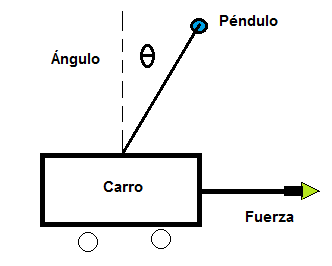
\includegraphics[scale=0.70]{pendulo1}
\caption{Diagrama simple del P'endulo.}
\label{fig:pendulo1}
\end{figure}

\section{Justificaci'on}

Al conseguir los objetivos del proyecto, se desea demostrar que es posible controlar un sistema de control de din'amica r'apida a trav'es de una red de campo (basada en una capa f'isica o de enlace).

Por las caracter'isticas ampliamente estudiadas del p'endulo invertido, siendo 'este una planta no lineal de segundo orden, y considerando que muchos sistemas f'isicos reales son similares, esta planta se convierte en un sistema 'util para el ensayo de soluciones de control, as'i como  para el desarrollo de sistemas de control m'as eficientes.

Este proyecto permitir'a cumplir dos metas: 
\begin{itemize}
	\item Afianzar el conocimiento te'orico adquirido por el estudiante a trav'as de la implementaci'on de sistemas reales.
 \item Servir como plataforma para el ensayo de nuevas soluciones de control obtenidas a trav'as de la investigaci'on.
\end{itemize}

\section{Alcance}


La construcci'on del p'endulo constituye un proyecto impulsado por el grupo de investigaci'on en control y optimizaci'on de la UTN en el que se podr'a probar diferentes t'ecnicas de dise'no de controladores tales como control 'optimo y control por posicionamiento de polos (espacio de estados);  implementaci'on de observadores y observadores 'optimos. Todo esto en base a funciones de transferencia sustentadas matem'aticamente que podr'ian comprender el modelado de retardos de propagaci'on y procesamiento. Se pondra a prueba el sistema con un controlador basado en t'ecnicas de estado de espacios; con lo cual se validar'a la funcionalidad de todo el sistema.


El control a implementarse en el p'endulo se realizar'a a trav'es de varios sistemas microprocesados comunicados mediante una red de campo (control distribuido).
Adem'as la planta contar'a con una HMI (interfaz humano-m'aquina) implementada en un ordenador, con el fin de establecer un sistema de supervisi'on y adquisici'on de datos del p'endulo para un posterior an'alisis off-line. Todo los sistemas es basar'an en software y hardware libre.

\section{Datos generales}
\subsection{Sistema Mec'anico}
El sistema mec'anico as'i como los componentes del mismo est'an descritos a detalle en la tesis que precede a 'este trabajo; conformado de: una mesa, un sistema de rieles que permiten la movilidad, un carro, un sistema eje-p'endulos, sensores de posici'on y un sistema de transmisi'on de fuerza con un motor acoplado.

\subsection{Sistema Electr'onico y de Control}
En breves rasgos el sistema electr'onico esta compuesto por placas 4 ``Arduinos Uno'' montadas en una red CAN. Cada nodo a detalle ser'a explicado en posteriores cap'itulos; pero b'asicamente los nodos 1 y 2 obtendra datos de los sensores los procesar'a y convertir'a pertinentemente a las unidades adecuadas; el nodo central o nodo 0 procesar'a estos datos y con ellos calcular'a una acci'on de control que ser'a enviada al nodo 3 donde se la convertir'a en voltaje para accionar el motor acoplado al sistema.
\chapter{Fundamento Te'orico}
\section{Dise'no del sistemas de control en espacio de estados}

\subsection{Asignaci'on de polos}

Todas las variables de estado con las que el sistema cuenta, se suponen medibles y disponibles para su realimentaci'on y si el sistema es completamente controlable, se pueden colocar los polos del sistema en cualquier posici'on dentro de una matriz de estado de ganancias (matriz de ganancias de a realimentaci'on de estados). Se consiguen estos polos a partir de la respuesta transitoria, as'i como de las respuestas de frecuencia. Seleccionando una matriz de ganancias apropiado se puede conseguir que los polos del sistema en lazo cerrado tengan una posici'on adecuada  \citep{ogata}.

\subsection{Dise'no mediante asignaci'on de polos}

Se deben especificar todos los polos en lazo cerrado del sistema, tomando en cuenta que para ello se deben tener medidas excelentes de las variables de estado o incluir un observador de estado en el sistema; a parte de que el requisito primordial es que el sistema sea completamente controlable \citep{ogata}.

Siendo un sistema de control con la forma:

\setlength{\parskip}{0.1cm}
\begin{center}
$
\left\lbrace
\begin{array}{ll}
\dot{x}=Ax+BU\\
y=Cx+DU
\end{array}
\right.
$
\end{center}
\setlength{\parskip}{0.1cm}
donde: $x=$vector de estado (vector de dimensi'on $n$)\\
			$y=$se'nal de salida (escalar)\\
			$u=$se'nal de control (escalar)\\
			$A=$matriz de coeficientes constantes $n*n$\\
			$B=$matriz de coeficientes constantes $n*1$\\
			$C=$matriz de coeficientes constantes $1*n$\\
			$D=$constantes (escalar)\\

Se selecciona la se'nal de control :
\begin{center} 
$u=-Kx$
\end{center}

Es decir que \textbf{u} es es un estado instant'aneo; siendo la matriz \textbf{K} de 1xn denominada como matriz de ganancia de realimentaci'on de estado. Sistema mostrado en la Fig. \ref{fig:siscerrado} \citep{ogata}.
\begin{figure}[ht]
	\centering
		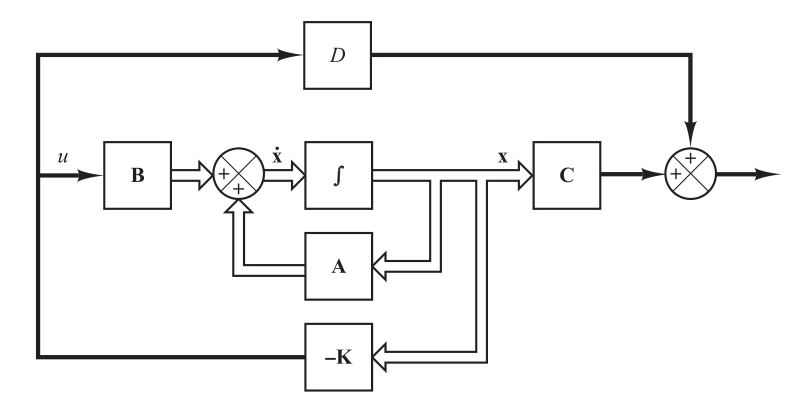
\includegraphics[scale=0.6]{sccerrado}
	\caption{Sistema de control en lazo cerrado}
	\label{fig:siscerrado}
\end{figure}

\setlength{\parskip}{0.4cm}

\section{Entorno de desarrollo integrado (IDE)}

El prop'osito m'as importante de un IDE es ayudar a acelerar el desarrollo preciso, r'apido y robusto de una aplicaci'on. Muchos IDEs se encuentran en desarrollo o est'an implementadas en universidades \citep{Ainternational}.

%%%%%%%%For most complex tasks, a combination of strategies is required. The ideal IDE will integrate shallow methods with methods based on tokens, patterns, grammars, keywords, logic, and finite state automata.It will integrate knowledge bases, expert systems, experts, planners, and other artificial intelligence systems with the overall framework 

\citet{kavitha} Muestra que algunos IDE contienen un compilador,int'erprete o ambos, como NetBeans y Eclipse. Muchos
IDEs modernos tambi'en tienen un navegador de clase,Y un diagrama de jerarqu'ia de clases.

\subsection{Entorno de desarrollo integrado abierto }

Open IDEs  son IDEs desarrollados, depurados y montados bajo una Licencia de Software de C'odigo Abierto, y permiten al programador de desarrollo de software nuevo, con todo tipo de licencias. Como PyCharm, NeatBeans, Matlab y otros.

\subsection{Herramientas de los IDEs }

``Hay muchas herramientas IDE disponibles para el c'odigo fuente
editor, herramientas de automatizaci'on y depurador. Algunos de los
Herramientas son, \textbf{\textsl{Eclipse,NetBeans, Code::Blocks, Code Lite, Dialog Blocks}}'' \citep{Ainternational}.
\begin{figure}[ht]
	\centering
		\includegraphics[scale=0.8]{idestop}
	\caption{Top 15 IDES. \smallskip Extraido de: \texttt{{http://pypl.github.io/IDE.html}}}
	\label{fig:idestop}
\end{figure}

Este top muestra la frecuencia con la que se realizan b'usquedas en IDE en Google. El 'indice puede ayudarle a decidir qu'e IDE utilizar \citep{pierre}. 

Como se puede ver en la Fig. \ref{fig:idestop} en la p'agina \pageref{fig:idestop}, est'an los IDE m'as importantes que se buscan en Google, y est'an  clasificadas por el lenguaje compatible como: ActionScript,	Ada,	Assembly,	BASIC,	C/C++,	C\#,	Common Lisp,	Component Pascal,	Eiffel,	Fortran, Haxe,	Java,	JavaScript,	Lua,	Pascal, Object Pascal,	Perl,	PHP,	Python,Racket,	Ruby,	Scala,	Small Basic,	Smalltalk,	Tcl.

En esta secci'on elegimos el lenguaje Python porque es una herramienta gratuita para el desarrollo y tambi'en es un lenguaje de programaci'on de alto nivel, de prop'osito general, interpretado y din'amico; todas estas particularidades hacen que este lenguaje sea perfecto para nuestro trabajo, y van a ser explicados en los siguientes cap'itulos.


\subsection{Software de c'odigo abierto}

El software de c'odigo abierto da acceso al c'odigo fuente; luego los usuarios pueden cambiar o modificar el producto original \citep{melissa}.

En otras palabras los usuarios tienen la libertad para ejecutar, copiar, distribuir, estudiar,
modificar y mejorar el software. Algunos autores lo
denominan ``software libre'' (tiene un contexto de libertad no de precio) \citep{anrango}. 

%%\subsubsection{Ideology}
%%%%%If you value fair use of information and intellectual freedom,
%open source software is right for you and your library. But
%remember, think of "free" as in freedom, not necessarily
%"free" as in price, although it often is. The free software
%movement differs slightly from open source software
%ideology in that free software promotes the freedom of all
%software everywhere and abhors proprietary software. Open
%source software proponents believe that this is not
%completely realistic and prefer promoting collaboration
%methods as superior to proprietary software. If a piece of
%software is called "free software," then it is also open source
%software. Live free, code free, improve the world \citep{melissa}.


\section{Lenguajes de programaci'on}
 
 
Lenguaje creado para para interpretar instrucciones elementales de la arquitectura mismo de los ordenadores; facilitando la tarea de programador, y que a partir de estos lenguajes se crean otros de nivel superior o lenguajes de alto nivel, que son mucho m'as productivos \citep{javier}.

 
\subsection{Paradigmas de programaci'on}

``Programming paradigms o Paradigmas de programaci'on'', seg'un \citet{javier} son patrones que moldean la forma de pensar y de formular soluciones asi como la de estructurar programas. Los paradigmas de programaci'on son: 
\begin{itemize}
\item Programaci'on imperativa. 
\item Programaci'on funcional. 
\item Programaci'on l'ogica. 
\item Programaci'on orientada a objetos.
\end{itemize}

\subsubsection{Lenguajes de alto nivel }
Del mismo modo \citep{javier} nos muestra que existen algunas caracter'isticas dentro de estos lenguajes:

Es un lenguaje independientes de la m'aquina, programas legibles y m'as f'aciles de entender; lenguajes m'as naturales; repertorio de instrucciones amplio, potente y f'acilmente utilizable;
 estructura pr'oxima a los lenguajes naturales, mantenimiento y correcci'on de errores m'as sencilla \citet{javier}.

\subsubsection{Traductores (Translators)}
Se establece que un traductor migra el programa creado de un lenguaje fuente a un lenguaje m'aquina. El proceso de conversi'on puede ser: por interpretaci'on o por compilaci'on \citep{javier}.
\subsubsection{Int'erpretes (Interpreters)}
Seg'un \citep{javier} es un programa que toma como entrada un programa escrito en lenguaje fuente y lo va
traduciendo y ejecutando instrucci'on por instrucci'on (de una en una).
\subsubsection{Compiladores (Compilers)}
Es un programa que toma como entrada un programa fuente y genera un programa
equivalente llamado programa objeto \citep{javier}.


\section{Python}
\subsection{Introducci'on}

Python nace en los noventa bajo la direccion de guido Van Rossum, es un lenguaje similar a Perl, pero con una sintaxis muy limpia y un c'odigo legible. Es un lenguaje interpretado, multiplataforma y orientada a objetos\citep{gonzales14}.

\subsection{Lenguaje interpretado o script}

Lenguaje que ejecuta un programa intermedio o de interpretaci'on en lugar de compilar a un lenguaje m'aquina, haciendo que este pueda ser interpretado directamente por la computadora. Python tiene muchas de las caracter'isticas de los lenguajes compilados, por lo que se podr'ia decir que es semi interpretado\citep{gonzales14}.


\subsection{Tipado din'amico}

Esta caracter'istica se refiere a que no es necesario declarar el tipo de dato de una variable, sino que este se determinar'a en tiempo de ejecuci'on; haciendo posible que el tipo de variable pueda cambiar con el tiempo \citep{gonzales14}.

\subsection{Tipado fuerte}

Es primordial convertir de forma expl'icita una variable a un nuevo tipo previo a su uso \citep{gonzales14}.

\subsection{Python}

Python deber'ia ser universal, su sintaxis es sencilla y clara; el tipado es fuerte, es orientada a objetos, tiene gran cantidad de librer'ias disponibles as'i como la calidad y potencia del lenguaje; por lo que desarrollar en python es una tarea sencilla \citep{gonzales14}.

Python es usado en Google, Yahoo, la NASA, Industrias Ligh \& Magic \citep{gonzales14}.

\begin{figure}[h]
	\centering
		
\includegraphics[scale=0.10]{Python_logo}
	\caption{Logo Python \texttrademark}
	\label{fig:Pythonlogo}
\end{figure}

\section{Sistemas operativos de tiempo real}

%\subsection{Introduction}

%Real­time and embedded computing applications in the first two computing era were rather rare and restricted
%to a few specialized applications such as space and defense. In the post­PC era of computing, the use of computer
%systems based on real­time and embedded technologies has already touched every facet of our life and is still growing
%at a pace that was never seen before. While embedded processing and Internet­enabled devices have now captured
%everyone's imagination, they are just a small fraction of applications that have been made possible by real­time
%systems. If we casually look around us, we can discover many of them ­ often they are camouflaged inside simple
%looking devices. If we observe carefully, we can notice several gadgets and applications which have today become indispensable to our every day life, are in fact based on embedded real­time systems. For example, we have ubiquitous
%consumer products such as digital cameras, cell phones, microwave ovens, camcorders, video game sets; telecommunication domain products and applications such as set­top boxes, cable modems, voice over IP (VoIP), and video
%conferencing applications; office products such as fax machines, laser printers, and security systems. Besides, we
%encounter real­time systems in hospitals in the form of medical instrumentation equipments and imaging systems.
%There are also a large number of equipments and gadgets based on real­time systems which though we normally do
%not use directly, but never the less are still important to our daily life. A few examples of such systems are Internet
%routers, base stations in cellular systems, industrial plant automation systems, and industrial robots \citep{mall}. 

%It can be easily inferred from the above discussion that in recent times real­time computers have become ubiquitous and have permeated large number of application areas. At present, the computers used in real­time applications
%vastly outnumber the computers that are being used in conventional applications. According to an estimate [3], 70\%
%of all processors manufactured world­wide are deployed in real­time embedded applications. While it is already true
%that an overwhelming majority of all processors being manufactured are getting deployed in real­time applications,
%what is more remarkable is the unmistakable trend of steady rise in the fraction of all processors manufactured
%world­wide finding their way to real­time applications \citep{mall}. 

%Some of the reasons attributable to the phenomenal growth in the use of real­time systems in the recent years 
%are the manifold reductions in the size and the cost of the computers, coupled with the magical improvements to
%their performance. The availability of computers at rapidly falling prices, reduced weight, rapidly shrinking sizes,
%and their increasing processing power have together contributed to the present scenario. Applications which not
%too far back were considered prohibitively expensive to automate, can now be affordably automated. For instance,
%when microprocessors costed several tens of thousands of Rupees, they were considered to be too expensive to be
%put inside a washing machine; but when they cost only a few hundred rupees, their use makes commercial sense \citep{mall}. 




\subsection{Definici'on}



As'i \citet{mall} define que un sistema se denomina sistema en tiempo real, cuando se necesita una expresi'on cuantitativa del tiempo (i.e. real-time) para describir el comportamiento de un sistema.

\citet{ortiz} nos brinda otro par de definiciones que son igualmente aceptables:

\begin{itemize}
	\item Un sistema a tiempo real debe producir tantas salidas como respuesta a unas entradas dentro de unos l'imites de tiempo plazos espec'ificos.
\item  Un sistema en tiempo real debe producir respuestas correctas dentro de unos limites de tiempo.
\end{itemize}

Pero de las cuales el mismo autor \citet{ortiz} se plantea un par de interrogantes derrivadas de estas definiciones, a las cuales 'el mismo da una respuesta:

\begin{itemize}
	\item ¿ Qu'e significa limites de tiempo espec'ificos?
	
	\begin{itemize}
		\item No necesitamos el mismo tiempo de respuesta en unas aplicaciones
que en otras.
	\end{itemize}
	\item¿ Por qu'e se dice ``debe producir'' y no dice ``produce''?

\begin{itemize}
	\item No en todas las aplicaciones es necesario que el sistema responda
siempre dentro de unos l'imites de tiempo concretos (ej. aplicaciones
multimedia), mientras que en otras es crucial (piloto autom'atico de
un avi'on).
\end{itemize}
\end{itemize}


\subsection{Aplicaciones}

Sobre las aplicaciones de los sistemas de tiempo real \citet{mall}  muestra algunos ejemplos, pero para el caso se presentaran solo dos ejemplos que ilustran la situaci'on de los sistemas operativos de tiempo real:

\subsubsection{Aplicaciones industriales}
Algunos ejemplos de aplicaciones industriales de sistemas en tiempo real son: sistemas de control de procesos, aplicaciones SCADA, equipos de prueba y medici'on, sistemas de automatizaci'on industrial y todos los materiales en equipos rob'oticos \citep{mall}.

\begin{itemize}
	\item \textbf{Ejemplo 1: Control de una planta qu'imica}\\
Un ordenador en tiempo real implementado en una planta qu'imica automatizada, monitorea peri'odicamente las condiciones de la planta como: lecturas actuales de presi'on, temperatura y concentraci'on qu'imica de la c'amara de reacci'on. Los par'ametros son muestreados peri'odicamente. Para mantener la reacci'on qu'imica a una determinada velocidad, la computadora en tiempo real decide las correcciones de las acciones necesarias, bas'andose en estos valores; cambiar la presi'on, temperatura u otros valores. En todos los sentidos, los l'imites de tiempo en un control de esta planta qu'imica var'ian desde unos pocos segundos hasta varios milisegundos \citep{mall}. 


\item \textbf{Ejemplo 2: Control, supervisi'on y Adquisici'on de Datos (SCADA )}\\
SCADA es una categor'ia de sistemas de control distribuidos que se utilizan en muchas industrias. Un sistema SCADA ayuda a supervisar y controlar un gran n'umero de eventos distribuidos de inter'es. En los sistemas SCADA, los sensores est'an dispersos en varios lugares geogr'aficos para recopilar datos en bruto (llamados eventos de inter'es). Estos datos se procesan a continuaci'on Y almacenados en una base de datos en tiempo real. Los eventos de inter'es est'an recibiendo datos de sensores en un sector espec'ifico dentro de una planta, luego se almacenan en una base de datos en tiempo real. Esta base de datos se est'a actualizando con frecuencia para convertirla en un modelo realista del estado de actualizaci'on del entorno. La restricci'on de tiempo en tal aplicaci'on SCADA es que los sensores deben detectar el estado del sistema a intervalos regulares (cada pocos milisegundos) y el mismo debe ser procesado antes de que se detecte el siguiente estado\citep{mall}.
\end{itemize}

Otros sistemas comunes de tiempo real dentro de algunas 'areas:

\begin{itemize}
	\item Sistemas de inyecci'on de conbustible multipunto.
	\item Impresora laser.

\item Video conferencias.
\item Celulares.
\item Sistemas de gu'ia de misiles.

\end{itemize}


\subsection{Modelo b'asico de un sistema en tiempo real}
\label{sec:ABasicModelOfARealTimeSystem}

\citet{mall}  explica el concepto b'asico sobre el modelo de un sistema en tiempo real:

\begin{figure}[ht]
	\centering
		\includegraphics[scale=0.7]{basic_realtimesystem}
	\caption{Modelo b'asico de un sistema en tiempo real}
	\label{fig:realtimesys}
\end{figure}

La Fig. \ref{fig:realtimesys} muestra un simple modelo b'asico de un sistema en tiempo real. \citet{mall} indica que  los sensores est'an interconectados con el bloque de acondicionamiento de entrada, que a su vez est'a conectado a la entrada interfaz. La interfaz de salida, el acondicionamiento de salida y el accionador est'an interconectados de una manera complementaria. A continuaci'on est'an brevemente los roles de los diferentes bloques funcionales de un sistema en tiempo real:

\textbf{Sensor:} Un sensor convierte alguna acci'on f'isica o caracter'istica de su entorno en se'nales el'ectricas \citep{mall}. 


\textbf{Actuador:} Un actuador es cualquier dispositivo que toma sus entradas de la interfaz de salida de un PC o microcontrolador y convierte estas se'nales el'ectricas en acciones f'isicas  \citep{mall}. 

\textbf{Acondicionamiento de se'nales:} \citet{mall} muestra que las se'nales el'ectricas producidas por un ordenador rara vez se pueden utilizar para accionar directamente un actuador por lo que es necesario algunos acondicionamientos realizados en se'nales brutas generadas por sensores y se'nales digitales generadas por computadoras.

\textbf{Conversi'on an'aloga-digital:} \citet{mall} explica que los ordenadores digitales no pueden procesar se'nales anal'ogicas. Por lo tanto, las se'nales anal'ogicas necesitan ser convertidas a forma digital. Las se'nales anal'ogicas pueden convertirse a forma digital utilizando un circuito cuyo diagrama de bloques se muestra en la Fig. \ref{fig:conversorad}. Utilizando el diagrama de bloques mostrado en Fig.\ref{fig:conversorad}, las se'nales anal'ogicas se convierten normalmente en forma digital a trav'es de los dos pasos principales siguientes:
\begin{figure}[ht]
	\centering
		\includegraphics[scale=0.8]{voltajecontinuo}
	\caption{Voltaje an'alogo continuo}
	\label{fig:voltajecontinuo}
\end{figure}


\begin{itemize}
	\item Muestra la se'nal anal'ogica (mostrado en la Fig. \ref{fig:voltajecontinuo}) a intervalos regulares. Este muestreo puede realizarse mediante un circuito de condensadores que almacena los niveles de voltaje. El nivel de voltaje almacenado puede ser discretizado. Despu'es de muestrear la se'nal anal'ogica, una forma de onda escalonada como se muestra en la Fig. \ref{fig:voltajedis} es obtenida \citep{mall}. 
\item Convierte el valor almacenado en un n'umero binario utilizando un convertidor anal'ogico a digital (ADC) como se muestra en la Fig. \ref{fig:conversorad} y almacenar el valor digital en un registro \citep{mall}. 

\end{itemize}

\begin{figure}[ht]
	\centering
		\includegraphics[scale=0.5]{voltajediscreto}
	\caption{Voltaje an'alogo convertido a la forma discreta}
	\label{fig:voltajedis}
\end{figure}

\begin{figure}[ht]
	\centering
		\includegraphics[scale=1]{conversorad}
	\caption{Conversi'on de una se'nal an'aloga a n'umero digital de 16 bits.}
	\label{fig:conversorad}
\end{figure}



\subsection{Tipos de tareas en tiempo real}

\subsubsection{Tareas del tipo hard}
Una tarea del tipo hard en tiempo real es aquella que est'a limitada a producir sus resultados dentro de ciertos l'imites de tiempo predefinidos. Se considera que el sistema ha fallado cuando alguna de sus tareas en tiempo real no 
produce los resultados requeridos antes del l'imite de tiempo especificado \citep{mall}. 
	
\subsubsection{Tareas del tipo firm }
Cada tarea en tiempo real del tipo firm est'a asociada con alg'un plazo predefinido antes del cual se producen sus resultados. Sin embargo, a diferencia de una tarea en tiempo real hard, incluso cuando una tarea en tiempo real firm no completa dentro su plazo la tarea requerida, el sistema no falla. Los resultados tard'ios son simplemente descartados. En otras palabras, la utilidad de los resultados calculados por una tarea en tiempo real firm se convierten en cero despu'es de la fecha l'imite. Se puede decir que si la respuesta en tiempo de una tarea excede el plazo especificado, entonces la utilidad de los resultados se convierte en cero y los resultados se descartan \citep{mall}.
\section{Open Hardware}

\subsection{Definici'on}

Aplicando ciertas libertades y definiciones antes dadas al software libre, entre ellas: libertad de uso, modificaci'on, distribuci'on y la redistribucion en mejoras con base al software original, con la diferencia de que para obtener un producto tangible tuvo que haber de antemano un sistema o proyecto con planos, estudios de costo, entre otras cosas. \citep{hernando}.

\citet{russell} presenta un resumen m'as espec'ifico sobre el "hardware abierto": El hardware de c'odigo abierto es un tipo de hardware en el que los esquemas y dise'nos se hacen sin restricciones y est'an disponibles para todos.
\subsection{Propiedades}
\citet{russell} da algunas propiedades del hardware abierto: Primero se acompa'nan a menudo del software abierto; Esto puede aportar fiabilidad y facilidad de depuraci'on. En segundo lugar Open Hardware viene con desarrollo modular para prototipos r'apidos usando bibliotecas preescritas.

El hardware de c'odigo abierto es hardware cuyo dise'no se hace disponible p'ublicamente para que cualquier persona pueda estudiar, modificar, distribuir, fabricar y vender el dise'no o el hardware basado en ese dise'no \citep{russell}.

\subsubsection{Hardware de c'odigo abierto}
Se refiere al hardware para el cual toda la informaci'on del dise'no se pone a
disposici'on del p'ublico en general. Open source hardware se puede basar en un
free hardware design, o el dise'no en el cual se basa puede ser restringido de
alguna manera  \citep{hernando}.

\subsubsection{Hardware libre}
Es un t'ermino usado de vez en cuando como sin'onimo para el open source
hardware; la cual busca ser directamente paralelo entre el hardware y el software. El t'ermino de
free hardware es particularmente confuso puesto que implica el estado f'isico del
hardware, m'as que su dise'no, el cual  es libre de alguna manera. Esto no es del
todo cierto en el sentido del costo, y tiene poca importancia en el sentido social.
Lo m'as simple es evitar este t'ermino totalmente, exceptuando su significado de
costo   \citep{hernando}.

\subsection{Hardware libre en Ecuador}
El inter'es de los modelos de Hardware Libre para Ecuador procede de su potencial como r'egimen de
producci'on y distribuci'on de tecnolog'ia, as'i como del desarrollo de nuevos
v'inculos sociales en torno a ella. El Hardware Libre tiene notables ventajas
comparativas, la situaci'on de partida del pa'is invita a prestar atenci'on al desarrollo de hardware libre con el objetivo de que su expansi'on favorezca el crecimiento econ'omico del en Ecuador, sin que tal desarrollo limite el
brillante potencial del Hardware Libre para la econom'ia del pa'is  \citep{lazalde}.


Actualmente existen muchos problemas para el desarrollo de un
hardware sustentable. Uno de los principales problemas son los altos costos de producci'on,
habitualmente derivados de la dependencia tecnol'ogica que afecta a muchos pa'ises, como
Ecuador \citep{lazalde}.

Por otra parte, los fabricantes de hardware y los titulares de los derechos de
autor aplican la Gesti'on de Derechos Digitales (DRM, por sus siglas en
ingl'es) para controlar el uso de contenidos y dispositivos digitales \citep{lazalde}.

Frente a esto, el Hardware Libre es relativamente barato y est'a profundamente integrado en los niveles de
alta innovaci'on. Adem'as, puede ser f'acilmente modificado a fin de
servir ciertos prop'ositos educativos \citep{lazalde}.


\section{Arduino}
\subsection{Introducci'on}
Entre las implementaciones de HL (Hardware Libre) m'as representativas est'a Arduino, una plataforma
inform'atica basada en un tablero microcontrolador simple y un ambiente de desarrollo para
escribir software en 'el. Est'a dirigido a artistas, dise'nadores, aficionados y
dem'as interesados en crear dispositivos o ambientes interactivos. Este microcontrolador
permite el funcionamiento de varios dispositivos derivados como el Arduino Geiger
(detector de radiaci'on), pHduino (medidor de pH), Xoscillo (osciloscopio) y OpenPCR
(an'alisis de ADN) \citep{lazalde}.

\citet{lazalde} exponen que Arduino bajo la licencia de Creative Commons "Attribution ShareAlike 3.0" (2010), lo que
significa que:
\begin{itemize}
	\item Quienquiera puede producir copias, redise'narlo o incluso vender placas de hardware.

\item Quienquiera que vuelva a publicar el dise'no de referencia debe atribuirlo al equipo original de Arduino.

\end{itemize}

\subsection{Asp'ectos T'ecnicos}


\citet{garcia} especifica la conformaci'on del Arduino :
El Arduino UNO es muy popular por su sencillez, coste y
dimensiones. Utiliza el microcontrolador ATmega328P, fabricado por ATMEL. Cuanta con las siguientes caracter'isticas t'ecnicas:

\begin{itemize}
	\item Voltaje: 5V.
\item Voltaje de entrada (recomendado): 7-12V.
\item Voltaje de entrada (l'imites): 6-20V.
\item Pines de entradas y salidas digitales: 14.
\item Corriente en pines de entrada y salida: 40mA.
\item Pines de entrada anal'ogica: 6.
\item Corriente en pin de 3.3V: 50mA.
\item Memoria Flash: 32KB.
\item SRAM: 2KB.
\item EEPROM: 1KB.
\item Velocidad reloj: 16MHz.
\item Dimensiones: 68.6x53.4mm.
\end{itemize}

\subsubsection{Arduino UNO Pinout Diagram}
\begin{figure}[h]
	\centering
		\includegraphics[scale=0.60]{Descripcionpines1}
	\caption{Arduino UNO Pinout Diagram}
	\label{fig:Descripcionpines}
\end{figure}
EL arduino IDE al momento de esta investigaci'on se encuentra en la versi'on 1.6.12 en su p'agina oficial.

\subsection{Arduino en Ecuador}
En Ecuador los estudiantes son los principales impulsodores del
desarrollo de proyectos de hardware libre. En la Campus Party celebrada en Quito en 2013, estudiantes
de la Universidad Polit'ecnica de Chimborazo, la Universidad T'ecnica de Loja y la
Universidad Salesiana de Quito desarrollaron dispositivos electr'onicos basados en Arduino.
Un ejemplo de Hardware Libre producido en el Ecuador es la aeronave no tripulada llamada Gavil'an UAV-2, dise'nada por las Fuerzas A'ereas Ecuatorianas (FAE) para vigilancia de 'areas de dif'icil acceso como la selva \citep{lazalde}.


\section{Red de 'area de comunicaci'on (CAN)}

\subsection{Can Bus Shield para Arduino: aspectos t'ecnicos}

El hardware que va a ser embebido en la placa de Arduino es un shield de marca SPARK FUN (CAN COMMUNICATION):
\begin{figure}[ht]
	\centering
		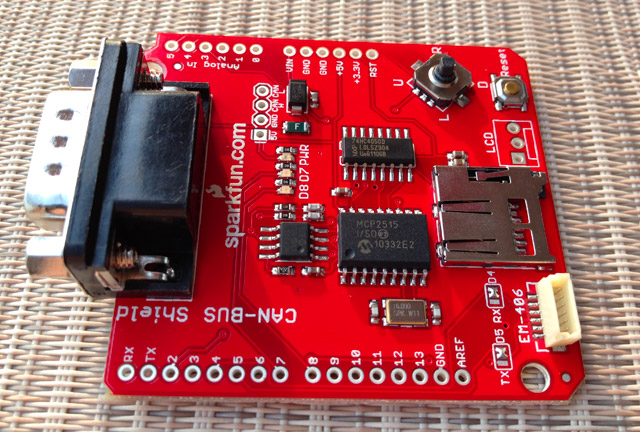
\includegraphics[scale=0.4]{shieldcan}
	\caption{CAN bus shield Sparkfun}
	\label{fig:sparkfun}
\end{figure}

Permite montar la red CAN con 4 nodos incrustados en ella. Consta de las siguientes caractr'isticas:

\begin{itemize}
	\item CAN v2.0B up to 1 Mb/s (1000Kbps).
	\item High speed SPI Interface (10 MHz) (with Arduino´s shield).
	\item Standard and extended data and remote frames.
	\item CAN connection via standard 9-way sub-D connector (DB-9).
	\item Power can supply to Arduino by sub-D via resettable fuse and reverse polarity protection.
	\item Socket for EM506 GPS module.
	\item Micro SD card holder.
	\item Connector for serial LCD.
	\item Reset button.
	\item Joystick control menu navigation control.
	\item Two LED indicator.
\end{itemize}
\begin{figure}[ht]
	\centering
		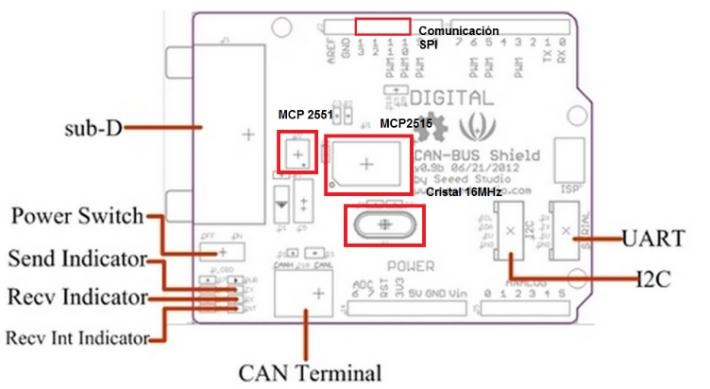
\includegraphics[scale=0.6]{canpartes}
	\caption{Partes del Shield CAN}
	\label{fig:canpartes}
\end{figure}





\subsection{Introducci'on}

El bus CAN  surge de la necesidad encontrar una forma de interconectar y conectar los distintos dispositivos de un autom'ovil en una sola red de una manera sencilla y reduciendo significativamente las conexiones, luego estandarizada en la norma ISO 11898-1; CAN bus cubre la capa de Enlace de datos y la F'isica  dentro de la pila de protocolo OSI \citep{garcia}.

%\begin{figure}[h]
	%\centering
		%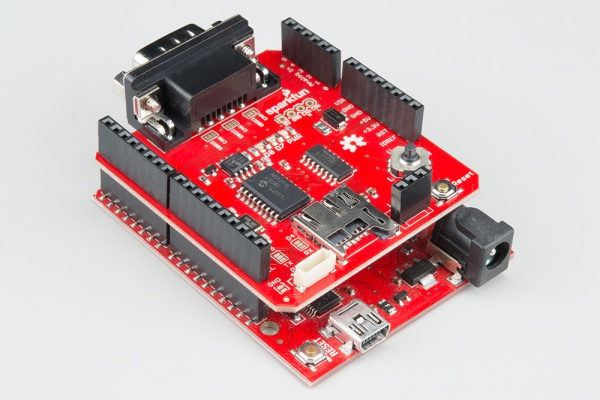
\includegraphics[scale=0.45]{canarduino}
	%\caption{\textit{CAN-BUS Shield} montado en un Arduino}
	%\label{fig:canarduino}
%\end{figure}


\subsection{Capa de enlace}
El protocolo de acceso es CSMA/CD + AMP (Carrier Sense Multiple
Access/ Collision Detection + Arbitration on Message Priority). Bajo este protocolo, los medios se ponen a la escucha de tramas de datos enviados en la red desde cualquier nodo, evitando as'i enviar mensajes mientras la red est'a ocupada; en el caso de que se envien mensajes al mismo tiempo desde dos o mas puntos de la red, el mensaje enviado es el que tenga como emisario al del identificador m'as bajo; cada nodo tiene un identificador que deber'a ser 'unico, es designado por software \citep{garcia}.


El campo de desici'on es al principio de la trama y la desici'on de prioridad se toma al final de la misma como se ve a continuaci'on:

\begin{figure}[ht]
	\centering
		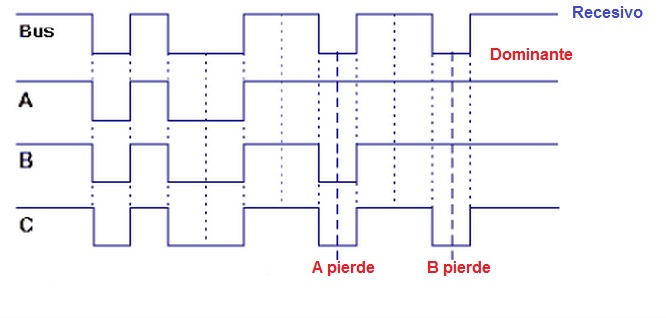
\includegraphics[scale=0.6]{Canynodos}
	\caption{Buffer de salida. Obtenido de \citet{garcia}.}
	\label{fig:canynodos}
\end{figure}

\subsection{Capa f'isica}

La capa f'isica debe recibir y enviar mensajes a la vez; a dem'as de presentar el estado recesivo y dominante en los nodos. tiene tres sub capas:

\subsubsection{PSL}
Physical Signaling Layer, sincroniza y temporiza los bits (modificaci'on por software) \citep{garcia}.
\subsubsection{PMA}
Convierte los niveles l'ogicos de transmisi'on y recepci'on  al lenguaje del protocolo \citep{garcia}.

\begin{figure}[ht]
	\centering
		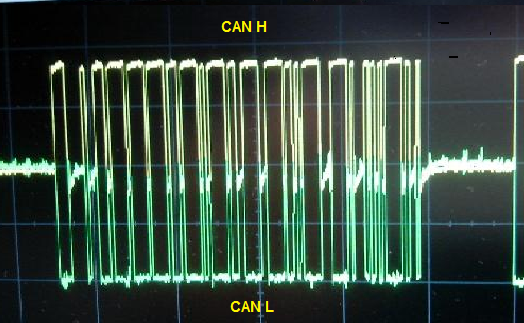
\includegraphics[scale=0.6]{canhcanl}
	\caption{Forma de onda generada por los canales de salida CAN H y CAN L \citep{garcia}.}
	\label{fig:canhcanl}
\end{figure}

La diferencia entre CAN H y CAN L que provee la comunicaci'on va de 0 a 2 volts, lo que da un nivel logico a un bit; el modo diferencial permite eliminar ruido \citep{garcia}.

\subsubsection{MDI}

Medium Dependent Interface, o interfaz dependiente del medio, indica como y bajo que medio se har'a la transmisi'on \citep{garcia}.

\begin{itemize}
\item Cables con resistencias de 120 $ \Omega $ .
\item Cable trenzado o apantallado.
\item Evitar derrivaciones.
\end{itemize}

\subsubsection{Trama de CAN bus}

El siguiente gra'afico representa una trama de datos de la comunicaci'on CAN:

\begin{figure}[ht]
	\centering
		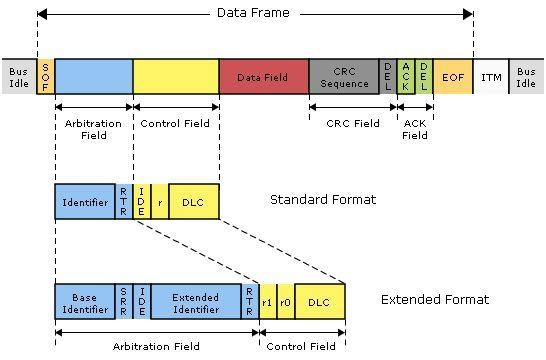
\includegraphics[scale=0.8]{tramacan}
	\caption{Trama generada en la comunicaci'on CAN\citep{garcia}.}
	\label{fig:tramacan}
\end{figure}

Consta de los siguientes elementos:

\begin{itemize}
\item SOF (Start of Frame bit).
\item Campo de arbitrio.
\item Campo de control.
\item Campo de datos.
\item Campo de verificaci'on por redundancia c'iclica CRC.
\item Campo de reconocimiento.
\item Campo de fin de trama.
\end{itemize}


\subsubsection{Trama remota}
Un nodo tiene la capacidad de solicitar un mensaje de otro nodo usando tramas remotas. Luego el nodo enviara su informaci'on al solicitante; el nodo que solicite la informaci'on deber'a tener el mismo identificador \citep{garcia}. Este tipo de trama no ser'a usada en el presente trabajo; en su lugar se utilizar'a una trama estandar de 8 bytes de datos.



\section{Driver, encoder, motor y finales de carrera}

El driver a utilizarse es DRIVER VNH2SP30, driver de hasta 16 volts. El encoder es HEDM-5500 con una resoluci'on de 2000 puntos cada 360° (2 encoders). El motor dc tiene una potencia de 180 watts a 24 volts. Finales de carrera del tipo mec'anico. Todos estos sensores y actuadores est'an descritos por \citet{montalvo} en la tesis previa a este trabajo y est'an montadas en el sistema mec'anico.

%\include{Objetivos}


%\include{antescedentes}
%\include{Problema}
%\include{justificacion}
%\include{Alcance}
%\include{datosgenerales}
%%%%%%%%%%%%%%%%%%%%%%%%%%%%%%%%%
%capitulo2}
%\chapter{Fundamento Te'orico}
\section{Dise'no del sistemas de control en espacio de estados}

\subsection{Asignaci'on de polos}

Todas las variables de estado con las que el sistema cuenta, se suponen medibles y disponibles para su realimentaci'on y si el sistema es completamente controlable, se pueden colocar los polos del sistema en cualquier posici'on dentro de una matriz de estado de ganancias (matriz de ganancias de a realimentaci'on de estados). Se consiguen estos polos a partir de la respuesta transitoria, as'i como de las respuestas de frecuencia. Seleccionando una matriz de ganancias apropiado se puede conseguir que los polos del sistema en lazo cerrado tengan una posici'on adecuada  \citep{ogata}.

\subsection{Dise'no mediante asignaci'on de polos}

Se deben especificar todos los polos en lazo cerrado del sistema, tomando en cuenta que para ello se deben tener medidas excelentes de las variables de estado o incluir un observador de estado en el sistema; a parte de que el requisito primordial es que el sistema sea completamente controlable \citep{ogata}.

Siendo un sistema de control con la forma:

\setlength{\parskip}{0.1cm}
\begin{center}
$
\left\lbrace
\begin{array}{ll}
\dot{x}=Ax+BU\\
y=Cx+DU
\end{array}
\right.
$
\end{center}
\setlength{\parskip}{0.1cm}
donde: $x=$vector de estado (vector de dimensi'on $n$)\\
			$y=$se'nal de salida (escalar)\\
			$u=$se'nal de control (escalar)\\
			$A=$matriz de coeficientes constantes $n*n$\\
			$B=$matriz de coeficientes constantes $n*1$\\
			$C=$matriz de coeficientes constantes $1*n$\\
			$D=$constantes (escalar)\\

Se selecciona la se'nal de control :
\begin{center} 
$u=-Kx$
\end{center}

Es decir que \textbf{u} es es un estado instant'aneo; siendo la matriz \textbf{K} de 1xn denominada como matriz de ganancia de realimentaci'on de estado. Sistema mostrado en la Fig. \ref{fig:siscerrado} \citep{ogata}.
\begin{figure}[ht]
	\centering
		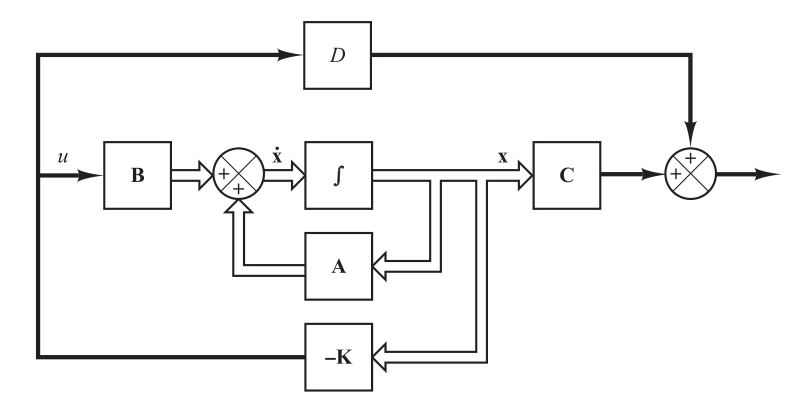
\includegraphics[scale=0.6]{sccerrado}
	\caption{Sistema de control en lazo cerrado}
	\label{fig:siscerrado}
\end{figure}

\setlength{\parskip}{0.4cm}

\section{Entorno de desarrollo integrado (IDE)}

El prop'osito m'as importante de un IDE es ayudar a acelerar el desarrollo preciso, r'apido y robusto de una aplicaci'on. Muchos IDEs se encuentran en desarrollo o est'an implementadas en universidades \citep{Ainternational}.

%%%%%%%%For most complex tasks, a combination of strategies is required. The ideal IDE will integrate shallow methods with methods based on tokens, patterns, grammars, keywords, logic, and finite state automata.It will integrate knowledge bases, expert systems, experts, planners, and other artificial intelligence systems with the overall framework 

\citet{kavitha} Muestra que algunos IDE contienen un compilador,int'erprete o ambos, como NetBeans y Eclipse. Muchos
IDEs modernos tambi'en tienen un navegador de clase,Y un diagrama de jerarqu'ia de clases.

\subsection{Entorno de desarrollo integrado abierto }

Open IDEs  son IDEs desarrollados, depurados y montados bajo una Licencia de Software de C'odigo Abierto, y permiten al programador de desarrollo de software nuevo, con todo tipo de licencias. Como PyCharm, NeatBeans, Matlab y otros.

\subsection{Herramientas de los IDEs }

``Hay muchas herramientas IDE disponibles para el c'odigo fuente
editor, herramientas de automatizaci'on y depurador. Algunos de los
Herramientas son, \textbf{\textsl{Eclipse,NetBeans, Code::Blocks, Code Lite, Dialog Blocks}}'' \citep{Ainternational}.
\begin{figure}[ht]
	\centering
		\includegraphics[scale=0.8]{idestop}
	\caption{Top 15 IDES. \smallskip Extraido de: \texttt{{http://pypl.github.io/IDE.html}}}
	\label{fig:idestop}
\end{figure}

Este top muestra la frecuencia con la que se realizan b'usquedas en IDE en Google. El 'indice puede ayudarle a decidir qu'e IDE utilizar \citep{pierre}. 

Como se puede ver en la Fig. \ref{fig:idestop} en la p'agina \pageref{fig:idestop}, est'an los IDE m'as importantes que se buscan en Google, y est'an  clasificadas por el lenguaje compatible como: ActionScript,	Ada,	Assembly,	BASIC,	C/C++,	C\#,	Common Lisp,	Component Pascal,	Eiffel,	Fortran, Haxe,	Java,	JavaScript,	Lua,	Pascal, Object Pascal,	Perl,	PHP,	Python,Racket,	Ruby,	Scala,	Small Basic,	Smalltalk,	Tcl.

En esta secci'on elegimos el lenguaje Python porque es una herramienta gratuita para el desarrollo y tambi'en es un lenguaje de programaci'on de alto nivel, de prop'osito general, interpretado y din'amico; todas estas particularidades hacen que este lenguaje sea perfecto para nuestro trabajo, y van a ser explicados en los siguientes cap'itulos.


\subsection{Software de c'odigo abierto}

El software de c'odigo abierto da acceso al c'odigo fuente; luego los usuarios pueden cambiar o modificar el producto original \citep{melissa}.

En otras palabras los usuarios tienen la libertad para ejecutar, copiar, distribuir, estudiar,
modificar y mejorar el software. Algunos autores lo
denominan ``software libre'' (tiene un contexto de libertad no de precio) \citep{anrango}. 

%%\subsubsection{Ideology}
%%%%%If you value fair use of information and intellectual freedom,
%open source software is right for you and your library. But
%remember, think of "free" as in freedom, not necessarily
%"free" as in price, although it often is. The free software
%movement differs slightly from open source software
%ideology in that free software promotes the freedom of all
%software everywhere and abhors proprietary software. Open
%source software proponents believe that this is not
%completely realistic and prefer promoting collaboration
%methods as superior to proprietary software. If a piece of
%software is called "free software," then it is also open source
%software. Live free, code free, improve the world \citep{melissa}.


\section{Lenguajes de programaci'on}
 
 
Lenguaje creado para para interpretar instrucciones elementales de la arquitectura mismo de los ordenadores; facilitando la tarea de programador, y que a partir de estos lenguajes se crean otros de nivel superior o lenguajes de alto nivel, que son mucho m'as productivos \citep{javier}.

 
\subsection{Paradigmas de programaci'on}

``Programming paradigms o Paradigmas de programaci'on'', seg'un \citet{javier} son patrones que moldean la forma de pensar y de formular soluciones asi como la de estructurar programas. Los paradigmas de programaci'on son: 
\begin{itemize}
\item Programaci'on imperativa. 
\item Programaci'on funcional. 
\item Programaci'on l'ogica. 
\item Programaci'on orientada a objetos.
\end{itemize}

\subsubsection{Lenguajes de alto nivel }
Del mismo modo \citep{javier} nos muestra que existen algunas caracter'isticas dentro de estos lenguajes:

Es un lenguaje independientes de la m'aquina, programas legibles y m'as f'aciles de entender; lenguajes m'as naturales; repertorio de instrucciones amplio, potente y f'acilmente utilizable;
 estructura pr'oxima a los lenguajes naturales, mantenimiento y correcci'on de errores m'as sencilla \citet{javier}.

\subsubsection{Traductores (Translators)}
Se establece que un traductor migra el programa creado de un lenguaje fuente a un lenguaje m'aquina. El proceso de conversi'on puede ser: por interpretaci'on o por compilaci'on \citep{javier}.
\subsubsection{Int'erpretes (Interpreters)}
Seg'un \citep{javier} es un programa que toma como entrada un programa escrito en lenguaje fuente y lo va
traduciendo y ejecutando instrucci'on por instrucci'on (de una en una).
\subsubsection{Compiladores (Compilers)}
Es un programa que toma como entrada un programa fuente y genera un programa
equivalente llamado programa objeto \citep{javier}.


\section{Python}
\subsection{Introducci'on}

Python nace en los noventa bajo la direccion de guido Van Rossum, es un lenguaje similar a Perl, pero con una sintaxis muy limpia y un c'odigo legible. Es un lenguaje interpretado, multiplataforma y orientada a objetos\citep{gonzales14}.

\subsection{Lenguaje interpretado o script}

Lenguaje que ejecuta un programa intermedio o de interpretaci'on en lugar de compilar a un lenguaje m'aquina, haciendo que este pueda ser interpretado directamente por la computadora. Python tiene muchas de las caracter'isticas de los lenguajes compilados, por lo que se podr'ia decir que es semi interpretado\citep{gonzales14}.


\subsection{Tipado din'amico}

Esta caracter'istica se refiere a que no es necesario declarar el tipo de dato de una variable, sino que este se determinar'a en tiempo de ejecuci'on; haciendo posible que el tipo de variable pueda cambiar con el tiempo \citep{gonzales14}.

\subsection{Tipado fuerte}

Es primordial convertir de forma expl'icita una variable a un nuevo tipo previo a su uso \citep{gonzales14}.

\subsection{Python}

Python deber'ia ser universal, su sintaxis es sencilla y clara; el tipado es fuerte, es orientada a objetos, tiene gran cantidad de librer'ias disponibles as'i como la calidad y potencia del lenguaje; por lo que desarrollar en python es una tarea sencilla \citep{gonzales14}.

Python es usado en Google, Yahoo, la NASA, Industrias Ligh \& Magic \citep{gonzales14}.

\begin{figure}[h]
	\centering
		
\includegraphics[scale=0.10]{Python_logo}
	\caption{Logo Python \texttrademark}
	\label{fig:Pythonlogo}
\end{figure}

\section{Sistemas operativos de tiempo real}

%\subsection{Introduction}

%Real­time and embedded computing applications in the first two computing era were rather rare and restricted
%to a few specialized applications such as space and defense. In the post­PC era of computing, the use of computer
%systems based on real­time and embedded technologies has already touched every facet of our life and is still growing
%at a pace that was never seen before. While embedded processing and Internet­enabled devices have now captured
%everyone's imagination, they are just a small fraction of applications that have been made possible by real­time
%systems. If we casually look around us, we can discover many of them ­ often they are camouflaged inside simple
%looking devices. If we observe carefully, we can notice several gadgets and applications which have today become indispensable to our every day life, are in fact based on embedded real­time systems. For example, we have ubiquitous
%consumer products such as digital cameras, cell phones, microwave ovens, camcorders, video game sets; telecommunication domain products and applications such as set­top boxes, cable modems, voice over IP (VoIP), and video
%conferencing applications; office products such as fax machines, laser printers, and security systems. Besides, we
%encounter real­time systems in hospitals in the form of medical instrumentation equipments and imaging systems.
%There are also a large number of equipments and gadgets based on real­time systems which though we normally do
%not use directly, but never the less are still important to our daily life. A few examples of such systems are Internet
%routers, base stations in cellular systems, industrial plant automation systems, and industrial robots \citep{mall}. 

%It can be easily inferred from the above discussion that in recent times real­time computers have become ubiquitous and have permeated large number of application areas. At present, the computers used in real­time applications
%vastly outnumber the computers that are being used in conventional applications. According to an estimate [3], 70\%
%of all processors manufactured world­wide are deployed in real­time embedded applications. While it is already true
%that an overwhelming majority of all processors being manufactured are getting deployed in real­time applications,
%what is more remarkable is the unmistakable trend of steady rise in the fraction of all processors manufactured
%world­wide finding their way to real­time applications \citep{mall}. 

%Some of the reasons attributable to the phenomenal growth in the use of real­time systems in the recent years 
%are the manifold reductions in the size and the cost of the computers, coupled with the magical improvements to
%their performance. The availability of computers at rapidly falling prices, reduced weight, rapidly shrinking sizes,
%and their increasing processing power have together contributed to the present scenario. Applications which not
%too far back were considered prohibitively expensive to automate, can now be affordably automated. For instance,
%when microprocessors costed several tens of thousands of Rupees, they were considered to be too expensive to be
%put inside a washing machine; but when they cost only a few hundred rupees, their use makes commercial sense \citep{mall}. 




\subsection{Definici'on}



As'i \citet{mall} define que un sistema se denomina sistema en tiempo real, cuando se necesita una expresi'on cuantitativa del tiempo (i.e. real-time) para describir el comportamiento de un sistema.

\citet{ortiz} nos brinda otro par de definiciones que son igualmente aceptables:

\begin{itemize}
	\item Un sistema a tiempo real debe producir tantas salidas como respuesta a unas entradas dentro de unos l'imites de tiempo plazos espec'ificos.
\item  Un sistema en tiempo real debe producir respuestas correctas dentro de unos limites de tiempo.
\end{itemize}

Pero de las cuales el mismo autor \citet{ortiz} se plantea un par de interrogantes derrivadas de estas definiciones, a las cuales 'el mismo da una respuesta:

\begin{itemize}
	\item ¿ Qu'e significa limites de tiempo espec'ificos?
	
	\begin{itemize}
		\item No necesitamos el mismo tiempo de respuesta en unas aplicaciones
que en otras.
	\end{itemize}
	\item¿ Por qu'e se dice ``debe producir'' y no dice ``produce''?

\begin{itemize}
	\item No en todas las aplicaciones es necesario que el sistema responda
siempre dentro de unos l'imites de tiempo concretos (ej. aplicaciones
multimedia), mientras que en otras es crucial (piloto autom'atico de
un avi'on).
\end{itemize}
\end{itemize}


\subsection{Aplicaciones}

Sobre las aplicaciones de los sistemas de tiempo real \citet{mall}  muestra algunos ejemplos, pero para el caso se presentaran solo dos ejemplos que ilustran la situaci'on de los sistemas operativos de tiempo real:

\subsubsection{Aplicaciones industriales}
Algunos ejemplos de aplicaciones industriales de sistemas en tiempo real son: sistemas de control de procesos, aplicaciones SCADA, equipos de prueba y medici'on, sistemas de automatizaci'on industrial y todos los materiales en equipos rob'oticos \citep{mall}.

\begin{itemize}
	\item \textbf{Ejemplo 1: Control de una planta qu'imica}\\
Un ordenador en tiempo real implementado en una planta qu'imica automatizada, monitorea peri'odicamente las condiciones de la planta como: lecturas actuales de presi'on, temperatura y concentraci'on qu'imica de la c'amara de reacci'on. Los par'ametros son muestreados peri'odicamente. Para mantener la reacci'on qu'imica a una determinada velocidad, la computadora en tiempo real decide las correcciones de las acciones necesarias, bas'andose en estos valores; cambiar la presi'on, temperatura u otros valores. En todos los sentidos, los l'imites de tiempo en un control de esta planta qu'imica var'ian desde unos pocos segundos hasta varios milisegundos \citep{mall}. 


\item \textbf{Ejemplo 2: Control, supervisi'on y Adquisici'on de Datos (SCADA )}\\
SCADA es una categor'ia de sistemas de control distribuidos que se utilizan en muchas industrias. Un sistema SCADA ayuda a supervisar y controlar un gran n'umero de eventos distribuidos de inter'es. En los sistemas SCADA, los sensores est'an dispersos en varios lugares geogr'aficos para recopilar datos en bruto (llamados eventos de inter'es). Estos datos se procesan a continuaci'on Y almacenados en una base de datos en tiempo real. Los eventos de inter'es est'an recibiendo datos de sensores en un sector espec'ifico dentro de una planta, luego se almacenan en una base de datos en tiempo real. Esta base de datos se est'a actualizando con frecuencia para convertirla en un modelo realista del estado de actualizaci'on del entorno. La restricci'on de tiempo en tal aplicaci'on SCADA es que los sensores deben detectar el estado del sistema a intervalos regulares (cada pocos milisegundos) y el mismo debe ser procesado antes de que se detecte el siguiente estado\citep{mall}.
\end{itemize}

Otros sistemas comunes de tiempo real dentro de algunas 'areas:

\begin{itemize}
	\item Sistemas de inyecci'on de conbustible multipunto.
	\item Impresora laser.

\item Video conferencias.
\item Celulares.
\item Sistemas de gu'ia de misiles.

\end{itemize}


\subsection{Modelo b'asico de un sistema en tiempo real}
\label{sec:ABasicModelOfARealTimeSystem}

\citet{mall}  explica el concepto b'asico sobre el modelo de un sistema en tiempo real:

\begin{figure}[ht]
	\centering
		\includegraphics[scale=0.7]{basic_realtimesystem}
	\caption{Modelo b'asico de un sistema en tiempo real}
	\label{fig:realtimesys}
\end{figure}

La Fig. \ref{fig:realtimesys} muestra un simple modelo b'asico de un sistema en tiempo real. \citet{mall} indica que  los sensores est'an interconectados con el bloque de acondicionamiento de entrada, que a su vez est'a conectado a la entrada interfaz. La interfaz de salida, el acondicionamiento de salida y el accionador est'an interconectados de una manera complementaria. A continuaci'on est'an brevemente los roles de los diferentes bloques funcionales de un sistema en tiempo real:

\textbf{Sensor:} Un sensor convierte alguna acci'on f'isica o caracter'istica de su entorno en se'nales el'ectricas \citep{mall}. 


\textbf{Actuador:} Un actuador es cualquier dispositivo que toma sus entradas de la interfaz de salida de un PC o microcontrolador y convierte estas se'nales el'ectricas en acciones f'isicas  \citep{mall}. 

\textbf{Acondicionamiento de se'nales:} \citet{mall} muestra que las se'nales el'ectricas producidas por un ordenador rara vez se pueden utilizar para accionar directamente un actuador por lo que es necesario algunos acondicionamientos realizados en se'nales brutas generadas por sensores y se'nales digitales generadas por computadoras.

\textbf{Conversi'on an'aloga-digital:} \citet{mall} explica que los ordenadores digitales no pueden procesar se'nales anal'ogicas. Por lo tanto, las se'nales anal'ogicas necesitan ser convertidas a forma digital. Las se'nales anal'ogicas pueden convertirse a forma digital utilizando un circuito cuyo diagrama de bloques se muestra en la Fig. \ref{fig:conversorad}. Utilizando el diagrama de bloques mostrado en Fig.\ref{fig:conversorad}, las se'nales anal'ogicas se convierten normalmente en forma digital a trav'es de los dos pasos principales siguientes:
\begin{figure}[ht]
	\centering
		\includegraphics[scale=0.8]{voltajecontinuo}
	\caption{Voltaje an'alogo continuo}
	\label{fig:voltajecontinuo}
\end{figure}


\begin{itemize}
	\item Muestra la se'nal anal'ogica (mostrado en la Fig. \ref{fig:voltajecontinuo}) a intervalos regulares. Este muestreo puede realizarse mediante un circuito de condensadores que almacena los niveles de voltaje. El nivel de voltaje almacenado puede ser discretizado. Despu'es de muestrear la se'nal anal'ogica, una forma de onda escalonada como se muestra en la Fig. \ref{fig:voltajedis} es obtenida \citep{mall}. 
\item Convierte el valor almacenado en un n'umero binario utilizando un convertidor anal'ogico a digital (ADC) como se muestra en la Fig. \ref{fig:conversorad} y almacenar el valor digital en un registro \citep{mall}. 

\end{itemize}

\begin{figure}[ht]
	\centering
		\includegraphics[scale=0.5]{voltajediscreto}
	\caption{Voltaje an'alogo convertido a la forma discreta}
	\label{fig:voltajedis}
\end{figure}

\begin{figure}[ht]
	\centering
		\includegraphics[scale=1]{conversorad}
	\caption{Conversi'on de una se'nal an'aloga a n'umero digital de 16 bits.}
	\label{fig:conversorad}
\end{figure}



\subsection{Tipos de tareas en tiempo real}

\subsubsection{Tareas del tipo hard}
Una tarea del tipo hard en tiempo real es aquella que est'a limitada a producir sus resultados dentro de ciertos l'imites de tiempo predefinidos. Se considera que el sistema ha fallado cuando alguna de sus tareas en tiempo real no 
produce los resultados requeridos antes del l'imite de tiempo especificado \citep{mall}. 
	
\subsubsection{Tareas del tipo firm }
Cada tarea en tiempo real del tipo firm est'a asociada con alg'un plazo predefinido antes del cual se producen sus resultados. Sin embargo, a diferencia de una tarea en tiempo real hard, incluso cuando una tarea en tiempo real firm no completa dentro su plazo la tarea requerida, el sistema no falla. Los resultados tard'ios son simplemente descartados. En otras palabras, la utilidad de los resultados calculados por una tarea en tiempo real firm se convierten en cero despu'es de la fecha l'imite. Se puede decir que si la respuesta en tiempo de una tarea excede el plazo especificado, entonces la utilidad de los resultados se convierte en cero y los resultados se descartan \citep{mall}.
\section{Open Hardware}

\subsection{Definici'on}

Aplicando ciertas libertades y definiciones antes dadas al software libre, entre ellas: libertad de uso, modificaci'on, distribuci'on y la redistribucion en mejoras con base al software original, con la diferencia de que para obtener un producto tangible tuvo que haber de antemano un sistema o proyecto con planos, estudios de costo, entre otras cosas. \citep{hernando}.

\citet{russell} presenta un resumen m'as espec'ifico sobre el "hardware abierto": El hardware de c'odigo abierto es un tipo de hardware en el que los esquemas y dise'nos se hacen sin restricciones y est'an disponibles para todos.
\subsection{Propiedades}
\citet{russell} da algunas propiedades del hardware abierto: Primero se acompa'nan a menudo del software abierto; Esto puede aportar fiabilidad y facilidad de depuraci'on. En segundo lugar Open Hardware viene con desarrollo modular para prototipos r'apidos usando bibliotecas preescritas.

El hardware de c'odigo abierto es hardware cuyo dise'no se hace disponible p'ublicamente para que cualquier persona pueda estudiar, modificar, distribuir, fabricar y vender el dise'no o el hardware basado en ese dise'no \citep{russell}.

\subsubsection{Hardware de c'odigo abierto}
Se refiere al hardware para el cual toda la informaci'on del dise'no se pone a
disposici'on del p'ublico en general. Open source hardware se puede basar en un
free hardware design, o el dise'no en el cual se basa puede ser restringido de
alguna manera  \citep{hernando}.

\subsubsection{Hardware libre}
Es un t'ermino usado de vez en cuando como sin'onimo para el open source
hardware; la cual busca ser directamente paralelo entre el hardware y el software. El t'ermino de
free hardware es particularmente confuso puesto que implica el estado f'isico del
hardware, m'as que su dise'no, el cual  es libre de alguna manera. Esto no es del
todo cierto en el sentido del costo, y tiene poca importancia en el sentido social.
Lo m'as simple es evitar este t'ermino totalmente, exceptuando su significado de
costo   \citep{hernando}.

\subsection{Hardware libre en Ecuador}
El inter'es de los modelos de Hardware Libre para Ecuador procede de su potencial como r'egimen de
producci'on y distribuci'on de tecnolog'ia, as'i como del desarrollo de nuevos
v'inculos sociales en torno a ella. El Hardware Libre tiene notables ventajas
comparativas, la situaci'on de partida del pa'is invita a prestar atenci'on al desarrollo de hardware libre con el objetivo de que su expansi'on favorezca el crecimiento econ'omico del en Ecuador, sin que tal desarrollo limite el
brillante potencial del Hardware Libre para la econom'ia del pa'is  \citep{lazalde}.


Actualmente existen muchos problemas para el desarrollo de un
hardware sustentable. Uno de los principales problemas son los altos costos de producci'on,
habitualmente derivados de la dependencia tecnol'ogica que afecta a muchos pa'ises, como
Ecuador \citep{lazalde}.

Por otra parte, los fabricantes de hardware y los titulares de los derechos de
autor aplican la Gesti'on de Derechos Digitales (DRM, por sus siglas en
ingl'es) para controlar el uso de contenidos y dispositivos digitales \citep{lazalde}.

Frente a esto, el Hardware Libre es relativamente barato y est'a profundamente integrado en los niveles de
alta innovaci'on. Adem'as, puede ser f'acilmente modificado a fin de
servir ciertos prop'ositos educativos \citep{lazalde}.


\section{Arduino}
\subsection{Introducci'on}
Entre las implementaciones de HL (Hardware Libre) m'as representativas est'a Arduino, una plataforma
inform'atica basada en un tablero microcontrolador simple y un ambiente de desarrollo para
escribir software en 'el. Est'a dirigido a artistas, dise'nadores, aficionados y
dem'as interesados en crear dispositivos o ambientes interactivos. Este microcontrolador
permite el funcionamiento de varios dispositivos derivados como el Arduino Geiger
(detector de radiaci'on), pHduino (medidor de pH), Xoscillo (osciloscopio) y OpenPCR
(an'alisis de ADN) \citep{lazalde}.

\citet{lazalde} exponen que Arduino bajo la licencia de Creative Commons "Attribution ShareAlike 3.0" (2010), lo que
significa que:
\begin{itemize}
	\item Quienquiera puede producir copias, redise'narlo o incluso vender placas de hardware.

\item Quienquiera que vuelva a publicar el dise'no de referencia debe atribuirlo al equipo original de Arduino.

\end{itemize}

\subsection{Asp'ectos T'ecnicos}


\citet{garcia} especifica la conformaci'on del Arduino :
El Arduino UNO es muy popular por su sencillez, coste y
dimensiones. Utiliza el microcontrolador ATmega328P, fabricado por ATMEL. Cuanta con las siguientes caracter'isticas t'ecnicas:

\begin{itemize}
	\item Voltaje: 5V.
\item Voltaje de entrada (recomendado): 7-12V.
\item Voltaje de entrada (l'imites): 6-20V.
\item Pines de entradas y salidas digitales: 14.
\item Corriente en pines de entrada y salida: 40mA.
\item Pines de entrada anal'ogica: 6.
\item Corriente en pin de 3.3V: 50mA.
\item Memoria Flash: 32KB.
\item SRAM: 2KB.
\item EEPROM: 1KB.
\item Velocidad reloj: 16MHz.
\item Dimensiones: 68.6x53.4mm.
\end{itemize}

\subsubsection{Arduino UNO Pinout Diagram}
\begin{figure}[h]
	\centering
		\includegraphics[scale=0.60]{Descripcionpines1}
	\caption{Arduino UNO Pinout Diagram}
	\label{fig:Descripcionpines}
\end{figure}
EL arduino IDE al momento de esta investigaci'on se encuentra en la versi'on 1.6.12 en su p'agina oficial.

\subsection{Arduino en Ecuador}
En Ecuador los estudiantes son los principales impulsodores del
desarrollo de proyectos de hardware libre. En la Campus Party celebrada en Quito en 2013, estudiantes
de la Universidad Polit'ecnica de Chimborazo, la Universidad T'ecnica de Loja y la
Universidad Salesiana de Quito desarrollaron dispositivos electr'onicos basados en Arduino.
Un ejemplo de Hardware Libre producido en el Ecuador es la aeronave no tripulada llamada Gavil'an UAV-2, dise'nada por las Fuerzas A'ereas Ecuatorianas (FAE) para vigilancia de 'areas de dif'icil acceso como la selva \citep{lazalde}.


\section{Red de 'area de comunicaci'on (CAN)}

\subsection{Can Bus Shield para Arduino: aspectos t'ecnicos}

El hardware que va a ser embebido en la placa de Arduino es un shield de marca SPARK FUN (CAN COMMUNICATION):
\begin{figure}[ht]
	\centering
		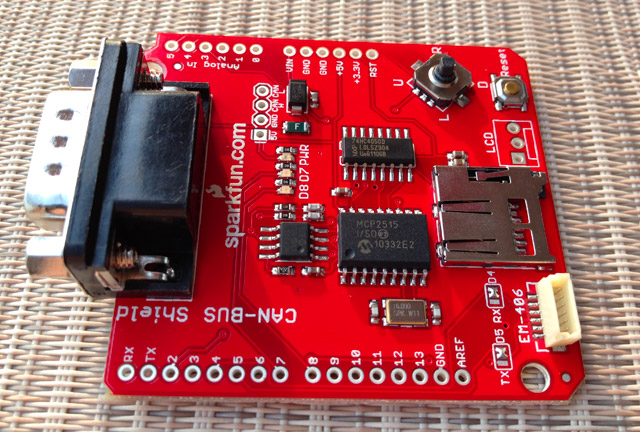
\includegraphics[scale=0.4]{shieldcan}
	\caption{CAN bus shield Sparkfun}
	\label{fig:sparkfun}
\end{figure}

Permite montar la red CAN con 4 nodos incrustados en ella. Consta de las siguientes caractr'isticas:

\begin{itemize}
	\item CAN v2.0B up to 1 Mb/s (1000Kbps).
	\item High speed SPI Interface (10 MHz) (with Arduino´s shield).
	\item Standard and extended data and remote frames.
	\item CAN connection via standard 9-way sub-D connector (DB-9).
	\item Power can supply to Arduino by sub-D via resettable fuse and reverse polarity protection.
	\item Socket for EM506 GPS module.
	\item Micro SD card holder.
	\item Connector for serial LCD.
	\item Reset button.
	\item Joystick control menu navigation control.
	\item Two LED indicator.
\end{itemize}
\begin{figure}[ht]
	\centering
		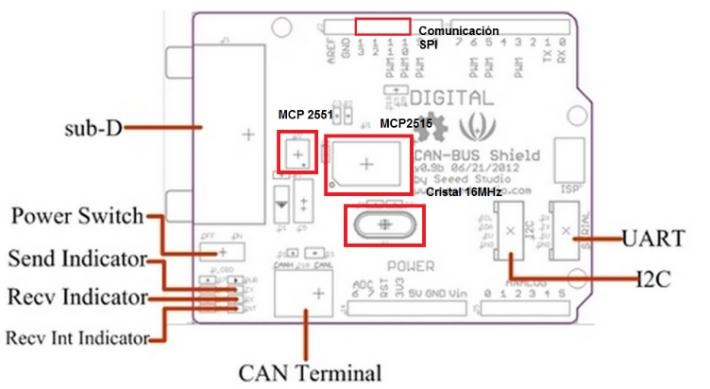
\includegraphics[scale=0.6]{canpartes}
	\caption{Partes del Shield CAN}
	\label{fig:canpartes}
\end{figure}





\subsection{Introducci'on}

El bus CAN  surge de la necesidad encontrar una forma de interconectar y conectar los distintos dispositivos de un autom'ovil en una sola red de una manera sencilla y reduciendo significativamente las conexiones, luego estandarizada en la norma ISO 11898-1; CAN bus cubre la capa de Enlace de datos y la F'isica  dentro de la pila de protocolo OSI \citep{garcia}.

%\begin{figure}[h]
	%\centering
		%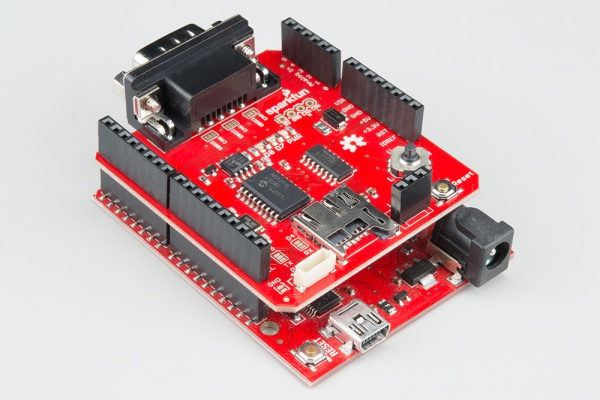
\includegraphics[scale=0.45]{canarduino}
	%\caption{\textit{CAN-BUS Shield} montado en un Arduino}
	%\label{fig:canarduino}
%\end{figure}


\subsection{Capa de enlace}
El protocolo de acceso es CSMA/CD + AMP (Carrier Sense Multiple
Access/ Collision Detection + Arbitration on Message Priority). Bajo este protocolo, los medios se ponen a la escucha de tramas de datos enviados en la red desde cualquier nodo, evitando as'i enviar mensajes mientras la red est'a ocupada; en el caso de que se envien mensajes al mismo tiempo desde dos o mas puntos de la red, el mensaje enviado es el que tenga como emisario al del identificador m'as bajo; cada nodo tiene un identificador que deber'a ser 'unico, es designado por software \citep{garcia}.


El campo de desici'on es al principio de la trama y la desici'on de prioridad se toma al final de la misma como se ve a continuaci'on:

\begin{figure}[ht]
	\centering
		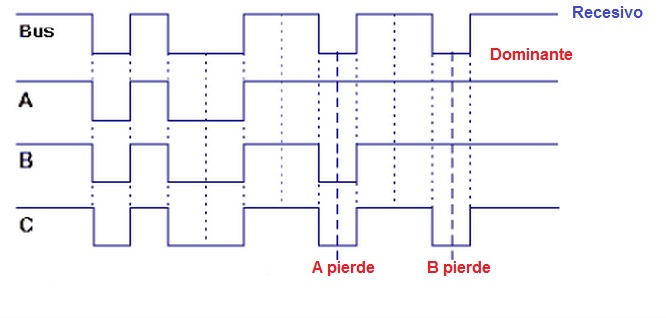
\includegraphics[scale=0.6]{Canynodos}
	\caption{Buffer de salida. Obtenido de \citet{garcia}.}
	\label{fig:canynodos}
\end{figure}

\subsection{Capa f'isica}

La capa f'isica debe recibir y enviar mensajes a la vez; a dem'as de presentar el estado recesivo y dominante en los nodos. tiene tres sub capas:

\subsubsection{PSL}
Physical Signaling Layer, sincroniza y temporiza los bits (modificaci'on por software) \citep{garcia}.
\subsubsection{PMA}
Convierte los niveles l'ogicos de transmisi'on y recepci'on  al lenguaje del protocolo \citep{garcia}.

\begin{figure}[ht]
	\centering
		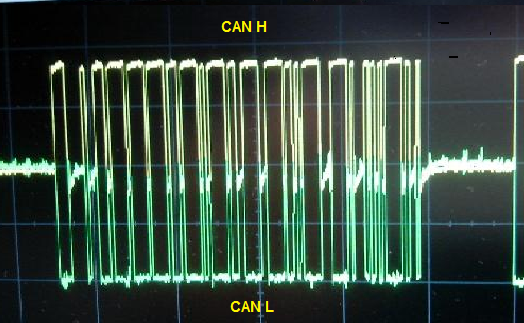
\includegraphics[scale=0.6]{canhcanl}
	\caption{Forma de onda generada por los canales de salida CAN H y CAN L \citep{garcia}.}
	\label{fig:canhcanl}
\end{figure}

La diferencia entre CAN H y CAN L que provee la comunicaci'on va de 0 a 2 volts, lo que da un nivel logico a un bit; el modo diferencial permite eliminar ruido \citep{garcia}.

\subsubsection{MDI}

Medium Dependent Interface, o interfaz dependiente del medio, indica como y bajo que medio se har'a la transmisi'on \citep{garcia}.

\begin{itemize}
\item Cables con resistencias de 120 $ \Omega $ .
\item Cable trenzado o apantallado.
\item Evitar derrivaciones.
\end{itemize}

\subsubsection{Trama de CAN bus}

El siguiente gra'afico representa una trama de datos de la comunicaci'on CAN:

\begin{figure}[ht]
	\centering
		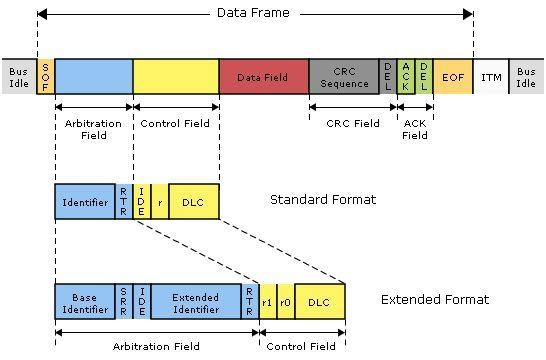
\includegraphics[scale=0.8]{tramacan}
	\caption{Trama generada en la comunicaci'on CAN\citep{garcia}.}
	\label{fig:tramacan}
\end{figure}

Consta de los siguientes elementos:

\begin{itemize}
\item SOF (Start of Frame bit).
\item Campo de arbitrio.
\item Campo de control.
\item Campo de datos.
\item Campo de verificaci'on por redundancia c'iclica CRC.
\item Campo de reconocimiento.
\item Campo de fin de trama.
\end{itemize}


\subsubsection{Trama remota}
Un nodo tiene la capacidad de solicitar un mensaje de otro nodo usando tramas remotas. Luego el nodo enviara su informaci'on al solicitante; el nodo que solicite la informaci'on deber'a tener el mismo identificador \citep{garcia}. Este tipo de trama no ser'a usada en el presente trabajo; en su lugar se utilizar'a una trama estandar de 8 bytes de datos.



\section{Driver, encoder, motor y finales de carrera}

El driver a utilizarse es DRIVER VNH2SP30, driver de hasta 16 volts. El encoder es HEDM-5500 con una resoluci'on de 2000 puntos cada 360° (2 encoders). El motor dc tiene una potencia de 180 watts a 24 volts. Finales de carrera del tipo mec'anico. Todos estos sensores y actuadores est'an descritos por \citet{montalvo} en la tesis previa a este trabajo y est'an montadas en el sistema mec'anico.
%\include{2programminglanguage}
%\include{2algoritmosyprogramas}
%\include{2python}
%\include{2realtime}
%\include{2openhardware}
%\include{2arduino}
%\include{2Can}
%%%%%%%%%%%%%%%%%%%%%%%%%%%%%%%%%
\chapter{Metodolog'ia}

\section{Sistema de control}

\subsection{Funci'on de Transferencia}

\abovedisplayskip=0pt
\belowdisplayskip=0pt

El controlador est'a basado en un sistema de equilibrio en bajo o mejor llamado \textit{Down-position} o \textit{crank-down}; y cuya funci'on de transferencia obtenida en la tesis previa de \citet{montalvo}:
\setlength{\parskip}{0pt}
\begin{equation}\label{eq:1} 
\,\ddot{x}=\frac{F-ml(\ddot{\theta}\cos\theta+\dot{\theta}^{2}\sin{\theta})-f_{c}\dot{x}}{(M+m)}\\
\end{equation}
\myequations{Funci'on de transferencia aceleraci'on lineal}
\begin{equation}\label{eq:2}
\,\ddot{\theta}=\frac{mgl\sin{\theta}-ml\ddot{x}\cos{\theta}-f_{p}\dot{\theta}}{(I_{p}+ml^{2})}
\end{equation}
\myequations{Funci'on de transferencia aceleraci'on angular}
\setlength{\parskip}{0.4cm}
Cuyos par'ametros estan representados en el cuadro \ref{parametros} y son:
\begin{table}[ht]
\centering
\begin{tabular}{ll}
$x_{p}$ &  X-coordinate for center of gravity of pendulum.\\
$y_{p}$  & Y-coordinate for center of gravity of pendulum.\\
$x_{c}$  & X-coordinate for center of gravity of cart.\\
$y_{c}$  & Y-coordinate for center of gravity of cart.\\
$y_{pp}$  & Y-coordinate for pivot point.\\
$l$  & Distance from pendulum center of gravity to pivot point.\\
$\theta$  & Pendulum angle from positive Y-direction.\\
$m$  & Mass of pendulum (load and rod).\\
$M$  & Cart mass.\\
$F$  & Force applied to cart.\\
$V$  & Vertical reaction force from pendulum.\\
$H$  & Horizontal reaction force from pendulum.\\
$I_{p}$  & Moment of inertia for pendulum with respect to pivot point.\\
$f_{p}$  & Viscous friction for pendulum at pivot point.\\
$f_{c}$  & Dynamic friction for cart.\\
 
\end{tabular}
\caption{Par'ametros de la funci'on de transferencia}
\label{parametros}
\end{table}


\section{Punto de equilibrio del sistema}
La ecuaci'on \ref{eq:1} muestra la representaci'on del sistema de una forma no-lineal. 
Equilibrio est'a definido como un punto (o una curva) en donde todos los estados permanecen sin cambio, sus derivadas son ceros (0). Despu'es de que \ref{eq:1} haya sido reemplazada en \ref{eq:2} y viceversa aparece un nuevo sistema de ecuaciones: \\

\setlength{\parskip}{0pt}

\begin{equation}\label{eq:3}
\,\beta\ddot{x}=(I_{p}+ml^{2})(F+ml\dot{\theta}^{2}\sin{\theta}-f_{c}\dot{x})-ml\cos{\theta}(mgl\sin{\theta}-f_{c}\dot{\theta})
\end{equation}
\myequations{Ecuaci'on de equilibrio 1}

\begin{equation}\label{eq:4}
\,\beta\ddot{\theta}=(M+m)(mgl\sin{\theta}-f_{p}\dot{\theta})-ml\cos{\theta}(F+ml\dot{\theta}^{2}\sin{\theta}-f_{c}\dot{x}) 
\end{equation}
\myequations{Ecuaci'on de equilibrio 2}
\begin{equation}\label{eq:5}
\,\beta=(M+m)(I_{p}+ml^{2})-(ml\cos{\theta})^{2} 
\end{equation}
\myequations{Ecuaci'on de equilibrio 3}
\setlength{\parskip}{0.4cm}
Las condiciones de $\dot{x}=0$,$\dot{\theta}=0$ y $F=0$ entonces las ecuaciones \ref{eq:3} y \ref{eq:4} resultan:\\
\setlength{\parskip}{0pt}
\begin{equation}\label{eq:6}
\,\beta\ddot{x}=-ml\cos{\theta}(mgl\sin{\theta}-f_{c}\dot{\theta})=0
\end{equation}
\myequations{Ecuaci'on de equilibrio 1 con condiciones iniciales 0}
\begin{equation}\label{eq:7}
\,\beta\ddot{\theta}=(M+m)(mgl\sin{\theta})=0
\end{equation}
\myequations{Ecuaci'on de equilibrio 2 con condiciones iniciales 0}
\setlength{\parskip}{0.4cm}
Ya que $\beta\neq0$ los 'unicos puntos que satisfacen estas ecuaciones son $\theta=0$ y $\theta=\pi$.
Esto tiene sentido ya que el p'endulo puede permanecer directamente abajo; as'i como hacia arriba si nada lo perturba.

\subsection{Linealizaci'on en posici'on bajo}
Si el 'area enfocada para el controlador en bajo es ($\theta=\pi$, $\dot{\theta}_{0}=0$), entonces tiene sentido linealizar para estos puntos, definiendo $\theta$ como una desviaci'on de $\theta_{\pi}$.La linealizaci'on usando las series de Taylor se muestra a continuaci'on.
\setlength{\parskip}{0pt}
\begin{equation}\label{eq:8}
\,\sin{\theta} \approx \sin{\theta}_{0}+ \left. \frac{\mathrm{d} \sin{\theta}_{0}}{\mathrm{d} x}\right|_{\theta_{0}=\pi} *\theta + \varepsilon \approx 0-1*\theta=-\theta
\end{equation}
\myequations{Taylor $\sin{\theta}$}
\setlength{\parskip}{0.4cm}
\setlength{\parskip}{0pt}
\begin{equation}\label{eq:9}
\cos{\theta} \approx \cos{\theta}_{0}+ \left. \frac{\mathrm{d} \cos{\theta}_{0}}{\mathrm{d} x}\right|_{\theta_{0}=\pi} *\theta + \varepsilon \approx -1-0*\theta=-1
\end{equation}
\myequations{Taylor $\cos{\theta}$}
\setlength{\parskip}{0.4cm}

Para $(\theta_{0}=\pi,\dot{\theta_{0}}=0)$ las versiones de ecuaciones linealizadas de las ecuaciones \ref{eq:8} y \ref{eq:9} son:
\setlength{\parskip}{0pt}
\begin{equation}\label{eq:10} 
\,\ddot{x}=\frac{F+ml\ddot{\theta}-f_{c}\dot{x}}{(M+m)}\\
\end{equation}
\myequations{Funci'on de transferencia lineal de $\ddot{x}$}
\begin{equation}\label{eq:11}
\,\ddot{\theta}=\frac{-mgl\theta-ml\ddot{x}-f_{p}\dot{\theta}}{I_{p}+ml^{2}}
\end{equation}
\myequations{Funci'on de transferencia lineal de $\ddot{\theta}$}
\setlength{\parskip}{0.4cm}


Usando las ecuaciones \ref{eq:8} y \ref{eq:9} para encontrar el espacio de estados; tomando en cuenta que para ellos los t'erminos deben ser de bajo orden. Por tanto $\ddot{x}$ debe ser sustituido en \ref{eq:11} por $\ddot{\theta}$ de \ref{eq:10} y viceversa.

\setlength{\parskip}{0pt}

\begin{center}
$\ddot{\theta}(I_{p}+ml^{2})=-mgl\theta+ml(\frac{F+ml\ddot{\theta}-f_{c}\dot{x}}{(M+m)})-f_{p}\dot{\theta}$\\
$\Leftrightarrow $\\
$\ddot{\theta}(I_{p}+ml^{2})(M+m)=(M+m)(-mgl\theta-f_{p}\dot{\theta})+ml(F+ml\ddot{\theta}-f_{c}\dot{x})$\\
$\Leftrightarrow $\\
$\ddot{\theta}((I_{p}+ml^{2})(M+m)-m^{2}l^{2})=(M+m)(-mgl\theta-f_{p}\dot{\theta})+ml(F-f_{c}\dot{x})$\\
$\Rightarrow $\\
Si $\alpha=(I_{p}+ml^{2})(M+m)-m^{2}l^{2}$, entonces:\\
$\Rightarrow $\\
$\ddot{\theta}=(M+m)(\frac{-mgl\theta}{\alpha}-\frac{f_{p}\dot{\theta}}{\alpha})+ml(\frac{F}{\alpha}-\frac{f_{c}\dot{x}}{\alpha})$\\
\end{center}

Ahora $\dot{\theta}$ deber'a ser sustituido en \ref{eq:10}:

\begin{center}
$\ddot{x}(I_{p}+ml^{2})(M+m)=ml(-mgl\theta+ml\ddot{x}-f_{p}\dot{\theta})+(F-f_{c}\dot{x})(I_{p}+ml^{2})$\\
$\Leftrightarrow $\\
$\ddot{x}((I_{p}+ml^{2})(M+m)-m^{2}l^{2})=ml(-mgl\theta-f_{p}\dot{\theta})+(F-f_{c}\dot{x})(I_{p}+ml^{2})$\\
$\Rightarrow $\\
Si $\alpha=(I_{p}+ml^{2})(M+m)-m^{2}l^{2}$, entonces:\\
$\Rightarrow $\\
$\ddot{\theta}=ml(\frac{-mgl\theta}{\alpha}-\frac{f_{p}\dot{\theta}}{\alpha})+(F-f_{c}\dot{x})(\frac{I_{p}}{\alpha}+\frac{ml^{2}}{\alpha})$\\
\end{center}

\setlength{\parskip}{0.4cm}
Usando el vector:
\begin{center}
$X=[x,\dot{x},\theta,\dot{\theta}]$\\
\end{center}

El sistema linealizado en espacio de estados esta descrito por:

\begin{center}

$
\left\lbrace
\begin{array}{ll}
\dot{X}=A_{down}X+B_{down}U\\
Y=CX+DU
\end{array}
\right.
$

\end{center}
\setlength{\parskip}{0.4cm}

Donde A,B,C,D son matrices y vectores definidos por espacio de estados y son:


\begin{center}
$
A_{down}=\left[
\begin{array}{cccc}
0 & 1 & 0 & 0 \\
0 & -\frac{(I_{p}+ml^{2})f_{c}}{\alpha} & \frac{-m^{2}l^{2}g}{\alpha} & \frac{-mlf_{p}}{\alpha} \\
0 & 0 & 0 & 1 \\
0 & \frac{-mlf_{c}}{\alpha} & -\frac{(M+m)mlg}{\alpha} & -\frac{(M+m)f_{p}}{\alpha}\\
\end{array}
\right]
$
\end{center}

\begin{center}
$
B_{down}=\left[
\begin{array}{c}
0  \\
 \frac{(I_{p}+ml^{2})}{\alpha}\\
0 \\
\frac{ml}{\alpha} \\
\end{array}
\right]
\hspace{8pt}
C=\left[
\begin{array}{cccc}
1 & 0 & 0 & 0 \\
0 & 1 & 0 & 0 \\
0 & 0 & 1 & 0 \\
0 & 0 & 0 & 1 \\
\end{array}
\right]
\hspace{8pt}
D= 0
\hspace{8pt}
U= F
$
\end{center}

\subsection{Matriz num'erica con par'ametros del sistema}

Tomando los siguientes par'ametros descritos por \citet{montalvo} para las constantes del sistema mostrados en \ref{constantes} :

\begin{table}[ht]
\centering
\begin{tabular}{ll}
$M =$ &  0.972 Kg\\
$m =$  & 0.144 Kg\\
$L =$  & 0.38 m\\
$I_{p} =$  & 0.02627 Kg/rad\\
$f_{p} =$  & 0.01 Ns/rad\\
$f_{c} =$  & 1.1 Ns/m\\
 
\end{tabular}
\caption{Constantes del sistema}
\label{constantes}
\end{table}

Las matrices obtenidas son las siguientes:


\begin{center}
$
A_{down}=\left[
\begin{array}{cccc}
0 & 1 & 0 & 0 \\
0 & -06498 & -0.5930 & -0.011 \\
0 & 0 & 0 & 1 \\
0 & -1.21& -12.08 & -0.2253\\
\end{array}
\right]
$
\end{center}

\begin{center}
$
B_{down}=\left[
\begin{array}{c}
0  \\
 4.04\\
0 \\
1.10 \\
\end{array}
\right]
\hspace{8pt}
C=\left[
\begin{array}{cccc}
1 & 0 & 0 & 0 \\
0 & 1 & 0 & 0 \\
0 & 0 & 1 & 0 \\
0 & 0 & 0 & 1 \\
\end{array}
\right]
\hspace{8pt}
D= 0
\hspace{8pt}
U= F
$
\end{center}

\section{Controlador del sistema en lazo cerrado}
El siguiente algoritmo est'a desarrollado en Matlab para obtener las ganancias para sistemas din'amicos en lazo cerrado:
{\tiny
\lstset{language=Matlab, breaklines=true, basicstyle=\footnotesize}
\begin{lstlisting}[frame=single]
%% 1. STATE FEEDBACK DISCRETE TIME CONTROLLER
clear all, close all, clc,

A=[0 1 0 0;0 -0.6498 -0.5930 -0.011; 0 0 0 1; 0 -1.21 -12.08 -0.2253];
B=[0;4.04;0;1.10];
C=[1 0 0 0; 0 1 0 0 ;0 0 1 0;0 0 0 1];
D=[0;0;0;0];

tTop = 0.3; %maximum time for simulation
h = 0.05; %sampling period (50msec)
tick = 0.01; %granularity

sys = ss(A, B, C, D);
sys_d = c2d(sys, h);

pole1 = -5+25j; %poles in continous time
pole2 = -5-25j;

z1 = exp(pole1*h); %poles in discrete time
z2 = exp(pole2*h);

K = acker(sys_d.a, sys_d.b, [z1 z2]); %controller design
CONTROLLER = K
\end{lstlisting}
}
\subsection{Ganancias obtenidas}
Estas son las ganancias obtenidas a partir del algoritmo de Matlab:
$G1=59.86$ (Ganancia de la posici'on del carro).\\
$G2=17.9$ (Ganancia de la velocidad del carro).\\
$G3=-3.17$ (Ganancia de la posici'on del p'endulo).\\
$G4=-10.713$ (Ganancia de la velocidad del p'endulo).\\
$G5=0.9345$ (Ganancia del error integral).

\section{Dise'no del sistema de control electr'onico y de comunicaci'on}

\subsection{Can Bus Shield}

El shield descrito en el cap'itulo anterior, conectar'a todos los nodos a continuaci'on descritos.
\begin{center}
\begin{figure}[ht]
	\centering
		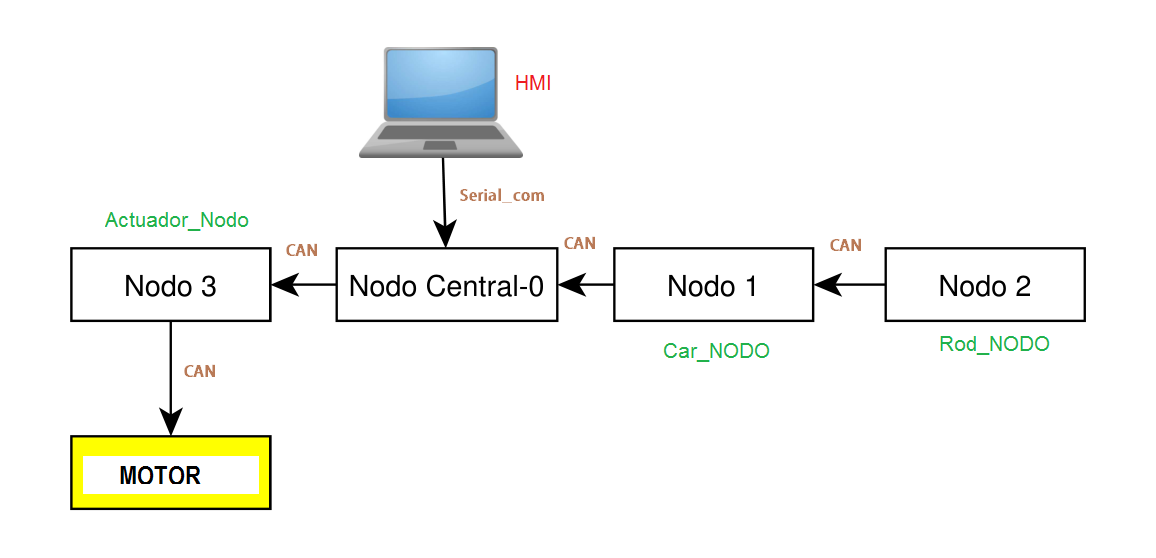
\includegraphics[width=14cm, height=7cm]{diagramacan}
	\caption{Diagrama general de la red}
	\label{fig:diagramacan}
\end{figure}
\end{center}


\subsection{Dise'no l'ogico general  de red}
Se prevee un esquema general de la red con todos sus nodos como se muestra en la Fig. \ref{fig:diagramacan}. Se utiliza el IDE de Arduino para el desarrollo del control de todos los nodos. El nodo primordial es el as'i llamado nodo central o nodo 0.

\begin{figure}[ht]
	\centering
		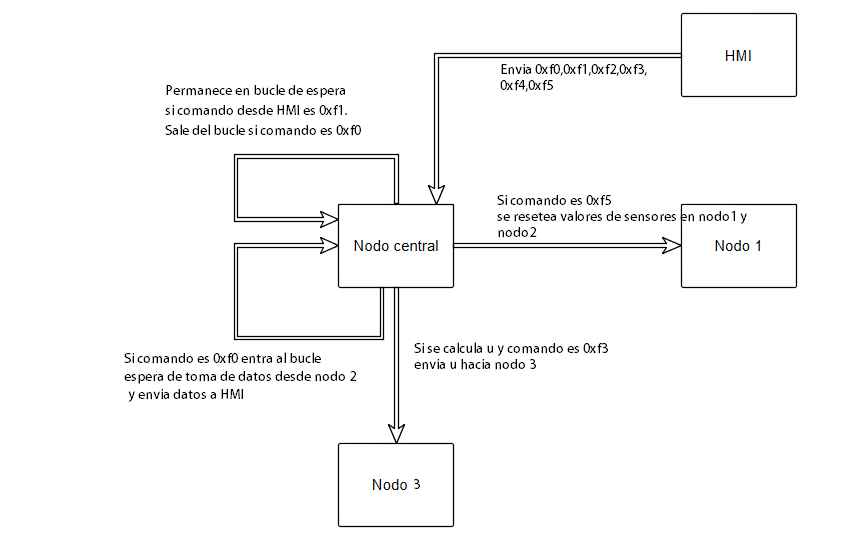
\includegraphics[scale=0.65]{nodocentral}
	\caption{Diagrama de m'aquina de estado del Nodo central}
	\label{fig:nodocentral}
\end{figure}

\subsection{Dise'no l'ogico de la estructura de la red: Nodo 0 }
En est'e nodo se realizar'an las acciones de control en base a la informaci'on proveniente del nodo 2; se encapsular'a la acci'on de control y se enviar'a al nodo 3; tambi'en tendra la importante funci'on de servir de enlace entre la HMI y la red CAN enviando y recibiendo informaci'on desde y hacia la PC, por tanto este nodo es el que m'as carga de trabajo tendr'a, ya que experimentar'a dos tipos de comunicaci'on: CAN y serial y la misi'on de calcular el controlador para el sistema Fig. \ref{fig:nodocentral}.

\subsubsection{Programaci'on nodo 0}

{\tiny
\begin{lstlisting}[language=C]
// demo: CAN-BUS Shield, send data
#include "mcpointer-can.h"
#include <SPI.h>
#include "TimerOne.h"

boolean txOn = false;  // whether the frame is complete
unsigned char counterRx = 0;
unsigned char bufferRx[20] = {0,0,0,0,0,0,0,0,0,0,0,0,0,0,0,0,0,0,0,0};
unsigned char len = 0;
unsigned char buf[8]= {0,0,0,0,0,0,0,0};
float float0 = 0; //numbers to be sent
float float1 = 0;
unsigned char *pointer-float0 = (unsigned char *)&float0;
unsigned char *pointer-float1 = (unsigned char *)&float1;

float float2 = 0; //values of analog read for tests
float float3 = 0;//values of analog read for tests
float float4 = 0; //numbers to be received from HMI
float float5 = 10; //numbers to be received from HMI
unsigned char *pointer-float15 = (unsigned char *)&float5; ////numbers to be received time for sampling (ts)(float)
float float6 = 0; //numbers to be received from HMI
float float7 = 0; //numbers to be received  from HMI
float *pointer-float4 = (float *)&bufferRx[1]; //value of gain
float *pointer-float5 = (float *)&bufferRx[5]; // time sampling (10-50)
float *pointer-float6 = (float *)&bufferRx[1]; // on/off
float *pointer-float7 = (float *)&bufferRx[5]; //tipe of control

//numbers to be received  from CAN
float   float10=0;
float *pointer-float10 = (float *)&buf[0]; //value of Time sampling from CAN

float   float11=0; 
float *pointer-float11 = (float *)&buf[4]; //value of Time sampling from CAN

float dxSensor1[]={0,0};
float dxSensor2[]={0,0};
float  dxres1=0;
float  dxres2=0;
float  rtime;
unsigned char *pointer-dx1 = (unsigned char *)&dxres1;
unsigned char *pointer-dx2 = (unsigned char *)&dxres2;
unsigned char *pointer-rtime = (unsigned char *)&rtime;
int cont2=0;


// the cs pin of the version after v1.1 is default to D9
// v0.9b and v1.0 is default D10
const int SPI_CS_PIN = 10;
const int ledHIGH    = 1;

const int LED=8;
const int LED2=7;
int cont=0;
boolean ledON=1;
unsigned char stmp[8] = {0,0,0,0,0,0,0,0};
unsigned char stmp2[8] = {0,0,0,0,0,0,0,0};
MCpointer-CAN CAN(SPI_CS_PIN);                                    // Set CS pin

void setup()
{
   Timer1.initialize(140000);         // Dispara cada 140 ms
  Timer1.attachInterrupt(ISR_timer); // Activa la interrupcion y la asocia a ISR_Blin
    Serial.begin(115200);

    while (CAN_OK != CAN.begin(CAN_1000KBPS))              // init can bus : baudrate = 500k
    {

    }  
   CAN.sendMsgBuf(0x70,0, 8, stmp);
    
}
void ISR_timer()
   {
    
  unsigned char i; 
  unsigned char eof[4] = {'c','X','r','C'};
  dxSensor1[1]=float2;
  dxSensor2[1]=float3;
  dxres1=(dxSensor1[1]-dxSensor1[0])/float5;
  dxres2=(dxSensor2[1]-dxSensor2[0])/float5;
  
  //this is is for take values of analog in uncomment analog read
  float2=float2;
  float3=float3;
  float0 = float2;
  float1 = float3;
 
  //this is for test if HMI is sending the two first values 4 controls
  
  //float0 = float4;
  //float1 = float5;
  //this is for test if HMI is sending the two first values 4 control
  //float0 = float6;
  //float1 = float7;
  

    //Serial.println(CAN.getCanId());
    digitalWrite(LED,1);
    
  
     //delay(float5);                       // send data 100ms per cycle
     
 
    if (txOn)
  {
   
    for (i=0; i<4; i++)
      //Serial.write(*pointer-float0 + i);
      Serial.write(pointer-float0[i]);


    for (i=0; i<4; i++)
      //Serial.write(*pointer-float1 + i);
      Serial.write(pointer-float1[i]);

      
    for (i=0; i<4; i++)
      Serial.write(pointer-dx1[i]);

      
    for (i=0; i<4; i++)
      Serial.write(pointer-dx2[i]);
    
    for (i=0; i<4; i++)
      Serial.write(pointer-rtime[i]);
      
    for (i=0; i<4; i++)
      Serial.write(eof[i]);
      
   
  }
  
    if(float6==0){
      unsigned char p[4]={0,0,0,0};
      unsigned char e[4] = {'c','X','r','C'};
    for (i=0; i<4; i++)
      //Serial.write(*pointer-float0 + i);
      Serial.write(p[i]);


    for (i=0; i<4; i++)
      //Serial.write(*pointer-float1 + i);
      Serial.write(p[i]);

      
    for (i=0; i<4; i++)
      Serial.write(p[i]);

      
    for (i=0; i<4; i++)
      Serial.write(p[i]);
    
    for (i=0; i<4; i++)
      Serial.write(p[i]);
      
    for (i=0; i<4; i++)
      Serial.write(e[i]);
      
   
    }
  dxSensor1[0]=dxSensor1[1];
  dxSensor2[0]=dxSensor2[1]; 
 
    
    }
void loop()
{  
   interrupts();  
		read();
	rtime = millis(); 
 
}

void read(){
   // unsigned char len = 0;
   // unsigned char buf[8];
    
    if(CAN_MSGAVAIL == CAN.checkReceive())            // check if data coming
    {
      CAN.readMsgBuf(&len, buf);    // read data,  len: data length, buf: data buf
      unsigned char canId = CAN.getCanId();
       
      if(CAN.getCanId()==0x20){    
       float10=(*pointer-float10);
       float11=(*pointer-float11);
       // if(float5>=10){
       // CAN.sendMsgBuf(0x70,0, 8, stmp);
       // }

       float2=float10;
		u = -gain1*cartPos - gain2*cartVel - gain3*rodPos - gain4*rodVel + gain5*error;
    }
    digitalWrite(LED,1);
  }
  else{
     
      if(float6==1){
        CAN.sendMsgBuf(0x70,0, 8, stmp);
        CAN.sendMsgBuf(0x10,0, 8, stmp2);
        }
     }
  
   digitalWrite(LED,1);
   
}
int aux=0;
void serialEvent()
{
  digitalWrite(LED2,0);
 
  while (Serial.available())
  {
    
   digitalWrite(LED2,1);
    bufferRx[counterRx] = (unsigned char)Serial.read(); //get the new byte
    
    if (counterRx >= 8)
    {
      counterRx = 0;
       
       
      switch (bufferRx[0]) //analyze command on first byte
      {
        case 0xf0:
          txOn = true;
//          here make a union of bytes to build the float registers
     
          float4 = (*pointer-float4);
          float5 = (*pointer-float5);  
   //here we send the value of ts from HMI to CAN
          stmp[0] = pointer-float15[0];
          stmp[1] = pointer-float15[1];
          stmp[2] = pointer-float15[2];
          stmp[3] = pointer-float15[3];
          
            aux+=1;
        break;
        case 0xf2:
          txOn = true;
//          here make a union of bytes to build the float registers        
          float6 = (*pointer-float6);
          float7 = (*pointer-float7);  
          aux+=1;      
        break;   
        case 0xf1:
          txOn = false;
          aux=0;
        break;
      } 
    }
    else
      counterRx++;  
    }   
 }

 \end{lstlisting}
}

\subsubsection{Controlador implementado en el nodo 0}
'Este es el controlador del sistema implementado en el nodo 0.
{\footnotesize
\begin{lstlisting}[language=C]
u = -gain1*cartPos - gain2*cartVel - gain3*rodPos - gain4*rodVel + gain5*error;

 \end{lstlisting}
}



\subsubsection{Sistema el'ectrico del nodo 0}

A continuaci'on se detalla el sistema de conexi'on del sistema el'ectrico del nodo 0 en la Fig. \ref{fig:nodo0electric}:
\begin{center}
\begin{figure}[ht]
	\centering
		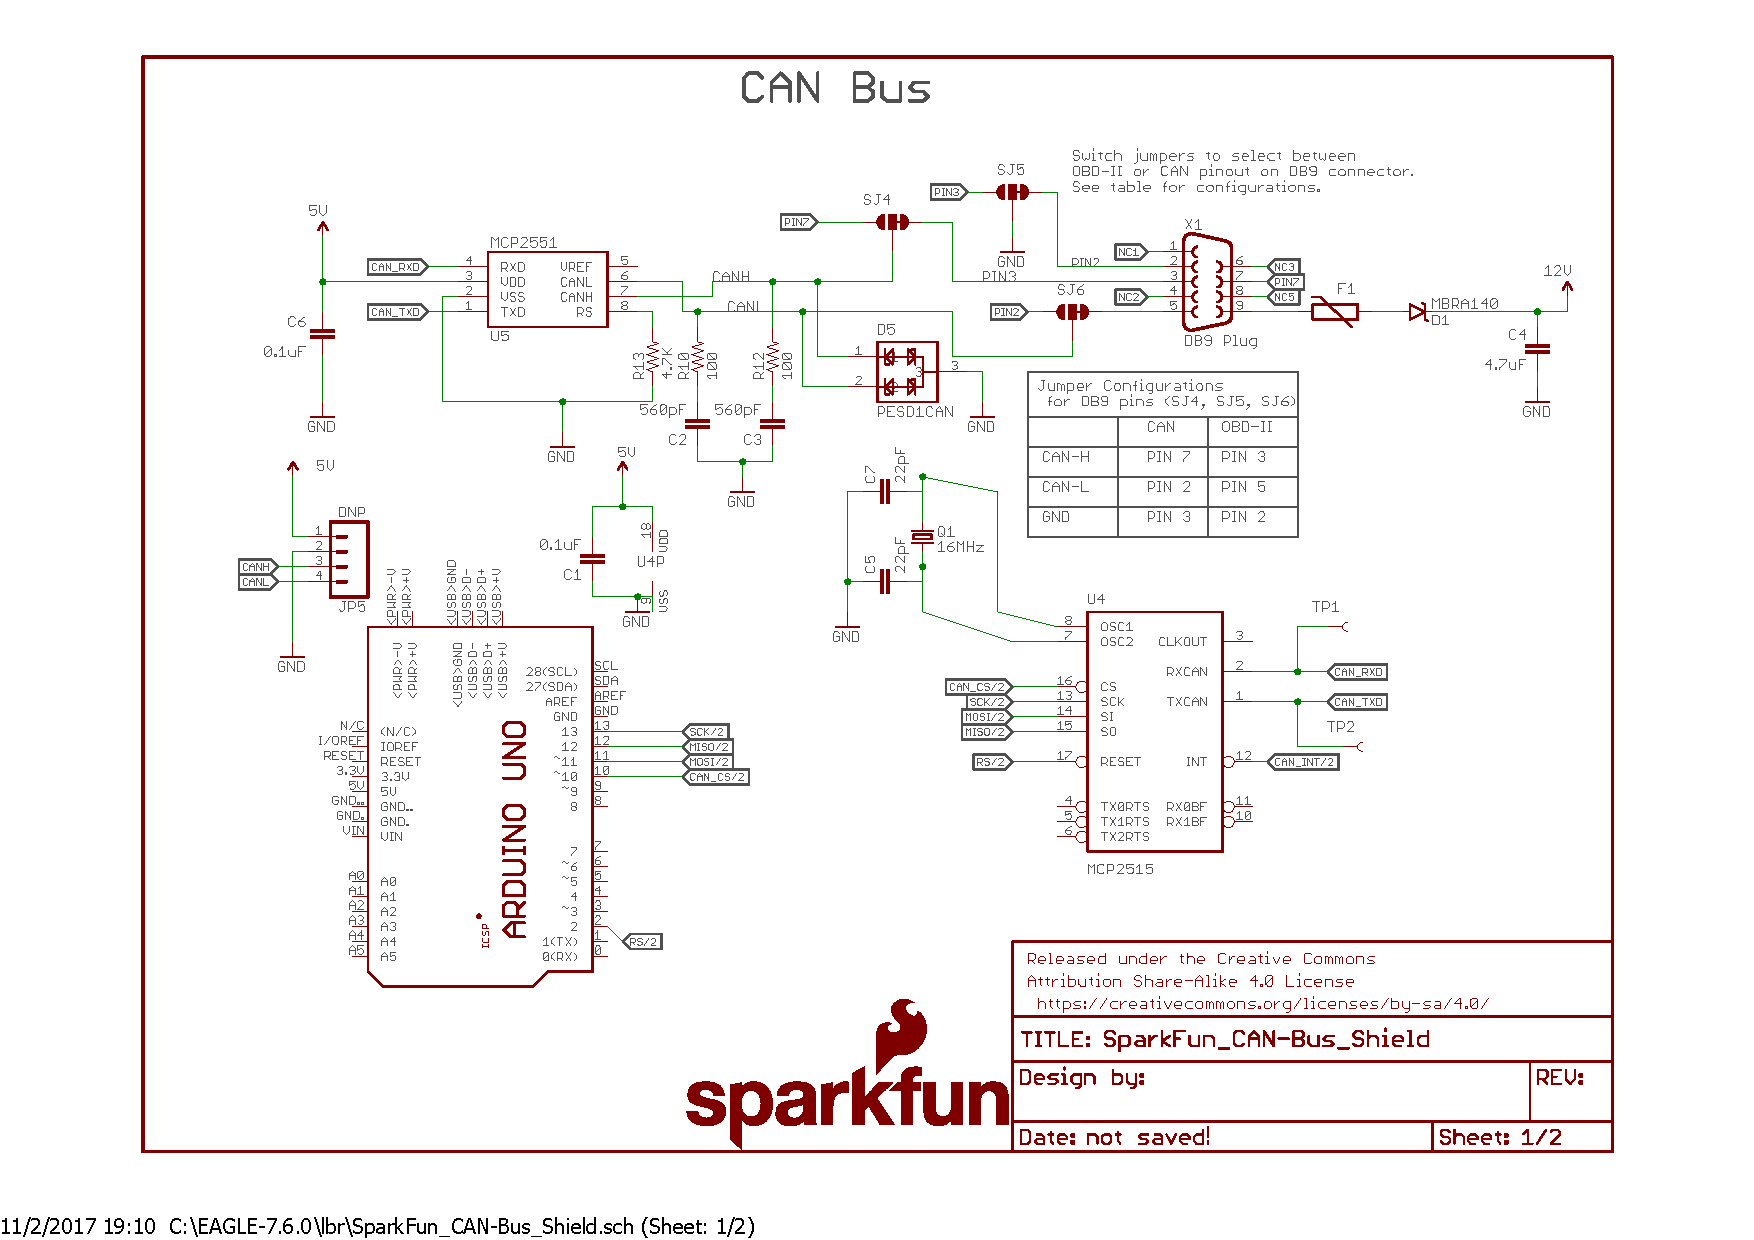
\includegraphics[width=14cm, height=10cm]{nodo0elec}
	\caption{Diagrama el'ectrico del nodo 0}
	\label{fig:nodo0electric}
\end{figure}
\end{center}

\subsection{Dise'no l'ogico de la estructura de la red: Nodo 1}

\subsubsection{M'aquina de estado Nodo 1}
En est'e nodo estar'a conectado el sensor ubicado en el motor con una particularidad, en este nodo se disparar'a las alarmas la toma de datos del sensor cada time sampling (ts) especificado en la HMI, que tendr'a que ser enviada primero al nodo central y luego a 'este; por defecto el nodo tiene un sampling de 10 (ms), siendo el rango permitido desde 10ms hasta 50 ms. En 'este nodo s'olomente se toman datos y se envian al nodo 2 como se muestra en la Fig. \ref{fig:nodo1}.Todas las librerias usadas se encuentran disponibles en la p'agina oficial de Arduino o en su defecto en la de terceros.
\begin{figure}[ht]
	\centering
		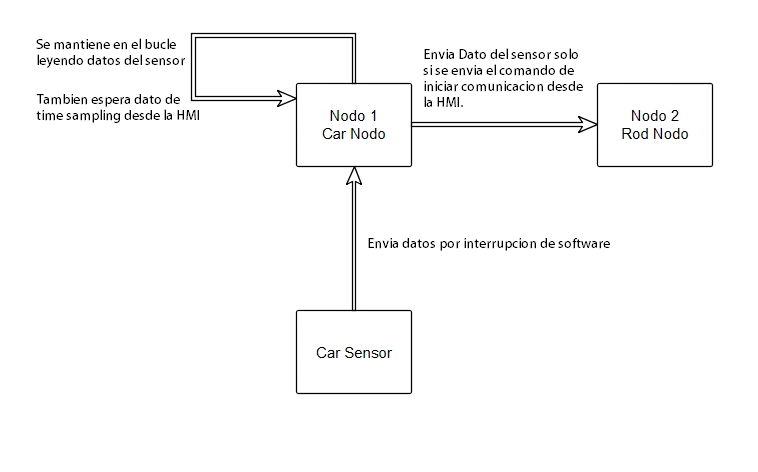
\includegraphics[scale=0.6]{nodo1}
	\caption{M'aquina de estado del Nodo 1}
	\label{fig:nodo1}
\end{figure}
\subsubsection{Programaci'on nodo 1}

Para el envio de datos se hace un direccionamiento indirecto; a continuaci'on toda la programaci'on: 

{\tiny

\begin{lstlisting}[language=C]

#include <SPI.h>
#include "mcpointer-can.h"
#include <Encoder.h>
#include <Timer.h>

Encoder myEnc(5, 6);
// the cs pin of the version after v1.1 is default to D9
// v0.9b and v1.0 is default D10
const int SPI_CS_PIN = 10;
const int LED=8;
unsigned char len = 0;
unsigned char buf[8]= {0,0,0,0,0,0,0,0};
boolean ledON=1;
float   float0=0;
unsigned char *pointer-float0 = (unsigned char *)&float0; //
unsigned long   float1=10; //this value never be less than 10 ms
unsigned long float2=10;

float *pointer-float1 = (float *)&buf[0]; //value of Time sampling from Central Controller 
int   aux=0;
float   aux2=0;
float   aux3=0;
float   aux4=0;
//int aux5=10;

Timer t;

unsigned char stmp[8] = {0, 0, 0, 0, 0, 0, 0, 0};
MCpointer-CAN CAN(SPI_CS_PIN);                                    // Set CS pin

void setup()
{
  //Timer1.initialize(10000);         // Dispara cada 10 ms
//  Timer1.attachInterrupt(ISR_timer); // Activa la interrupcion y la asocia a ISR_Blin
interrupts();
int tickEvent = t.every(float1, ISR_timer );   
    Serial.begin(115200);
    pinMode(LED,OUTPUT);
  
    while (CAN_OK != CAN.begin(CAN_1000KBPS))              // init can bus : baudrate = 500k
    {
       Serial.println("CAN BUS Shield init fail");
       Serial.println(" Init CAN BUS Shield again");
       // delay(100);
    }
    Serial.println("CAN BUS Shield init ok!");
    
}
void loop()
{
   
  int tickEvent = t.every(float1, ISR_timer );  
 // Timer1.stop();
 
 float0= myEnc.read();
  t.update();
  read(); 
 // delay(10);
 
}
void ISR_timer()
   {
    //float0= myEnc.read();
    
      Serial.println(float0);
      Serial.println(float1);
     //Serial.println(float1);
     //Serial.println(float2);
     //Serial.println(float3);
    
    
      //Timer1.restart();
    
  
  //  Serial.println(float2);

        stmp[0]= pointer-float0[0];
        stmp[1]= pointer-float0[1];
        stmp[2]=pointer-float0[2];
        stmp[3]=pointer-float0[3];
        CAN.sendMsgBuf(0x60,0, 8, stmp);    
   //Serial.println(float0);
    //Serial.println(float2);

   }
void read(){
   //unsigned char len = 0;
   // unsigned char buf[8];

    if(CAN_MSGAVAIL == CAN.checkReceive())            // check if data coming
    {
      CAN.readMsgBuf(&len, buf);    // read data,  len: data length, buf: data buf
      unsigned char canId = CAN.getCanId();
      // Serial.println(CAN.getCanId());
      if(CAN.getCanId()==0x70){
       
        float1=(*pointer-float1); //add to float1 the value of the pointer from de CAN buffer (time sampling).
        
         
         if(float1<=10) float1=10;
         if(float1>=50) float1=50;
         
         if(float2!=float1){
         
         Serial.println("TIme sampling has changed");
         }
         float2=float1;
    
    }
     digitalWrite(LED,1);
  }
  
  }

/*********************************************************************************************************
  END FILE
*********************************************************************************************************/

\end{lstlisting}
}
\subsubsection{Sistema el'ectrico del nodo 1}

A continuaci'on se detalla el sistema de conexi'on del sistema el'ectrico del nodo 1 en la Fig. \ref{fig:nodo1electric}:

\begin{center}
\begin{figure}[ht]
	\centering
		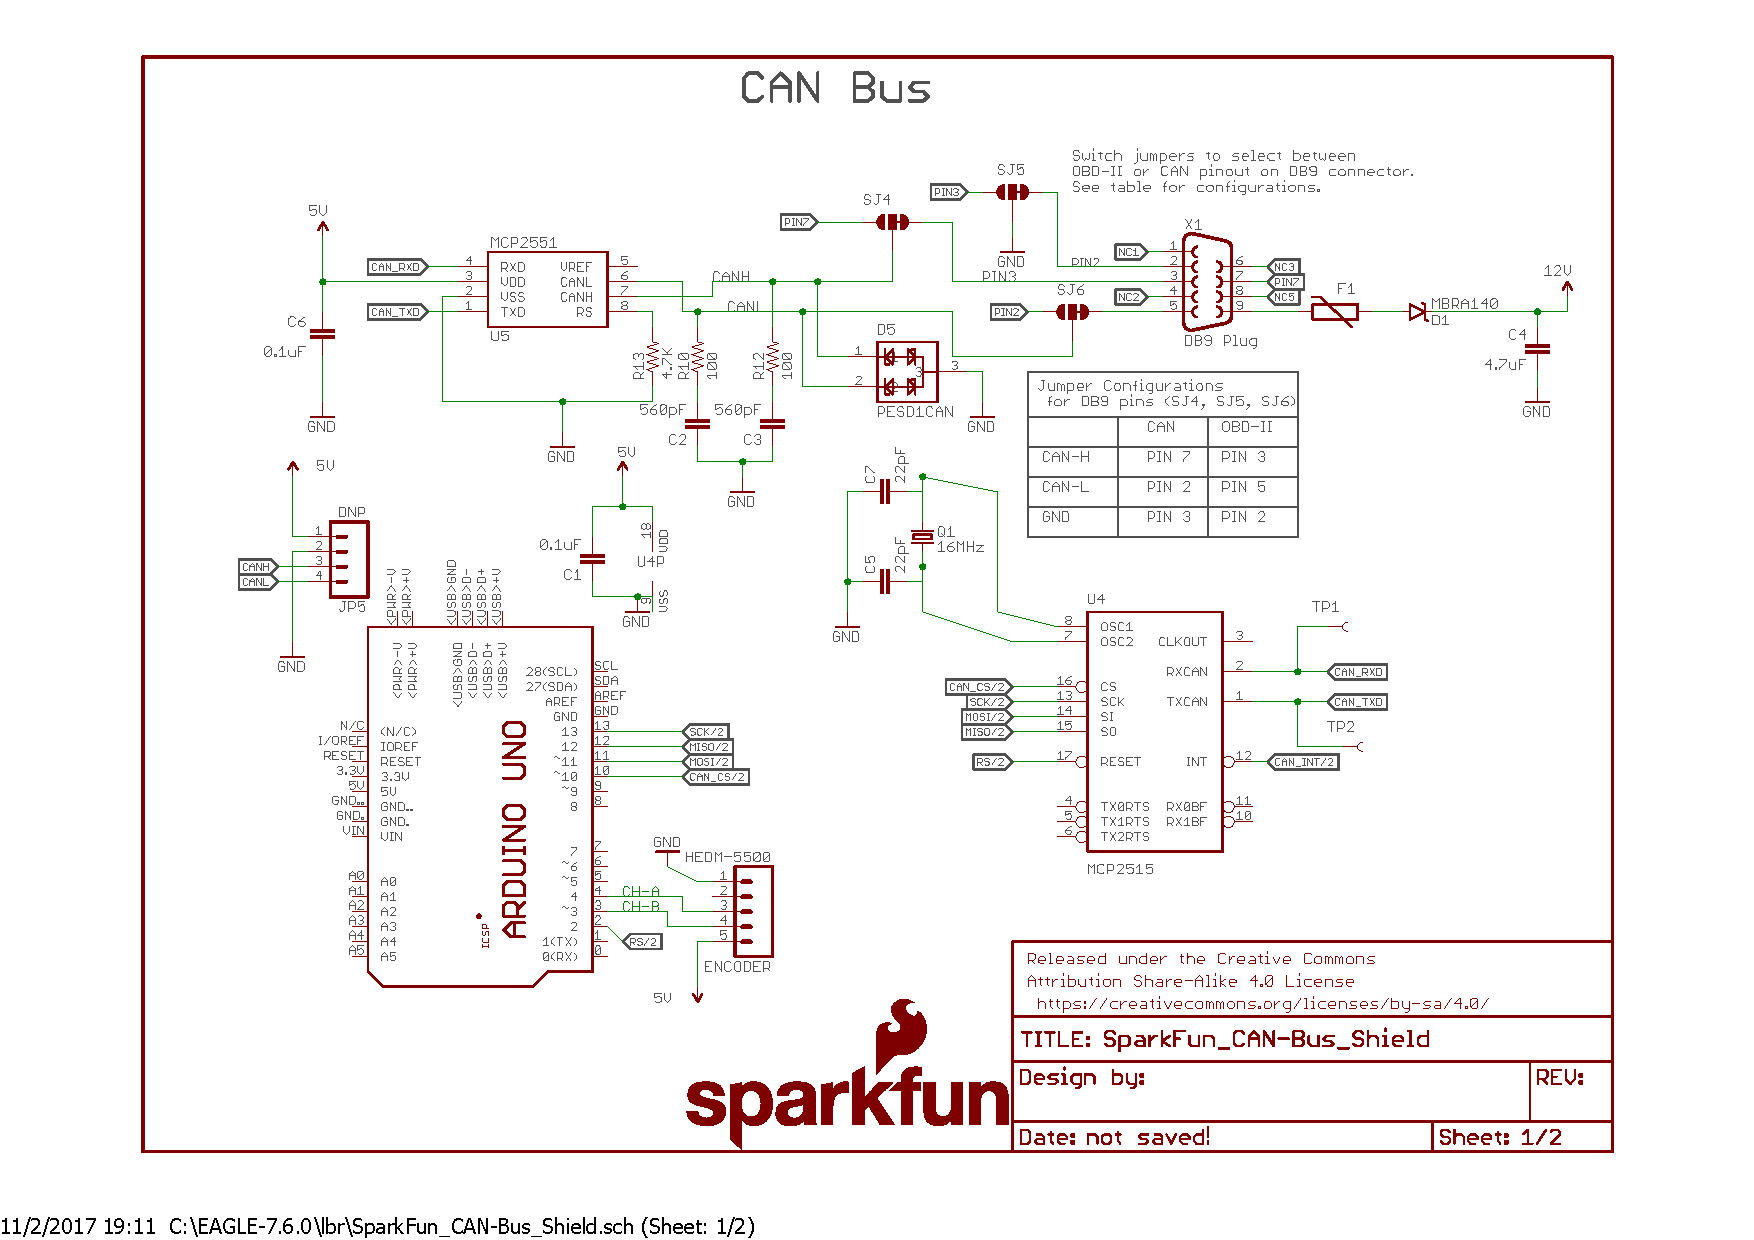
\includegraphics[width=14cm, height=10cm]{nodo1elec}
	\caption{Diagrama el'ectrico del nodo 1}
	\label{fig:nodo1electric}
\end{figure}
\end{center}

\subsection{Dise'no l'ogico de la estructura de la red: Nodo 2}

\subsubsection{M'aquina de estado del Nodo 2}
En este nodo se toman datos del sensor ubicado en el p'endulo con una particularidad; s'olo se disparar'a el envio de datos al nodo central cada vez que le llegue informaci'on del nodo 1; luego 'este tomar'a el dato del sensor, lo encapsular'a, lo pondr'a en la cola a continuaci'on de los datos del nodo 1 que pasan directamente de la entrada a la salida del buffer de la red y enviar'a ambos datos al nodo central, como se muestra en la Fig. \ref{fig:nodo2}.


\begin{figure}[ht]
	\centering
		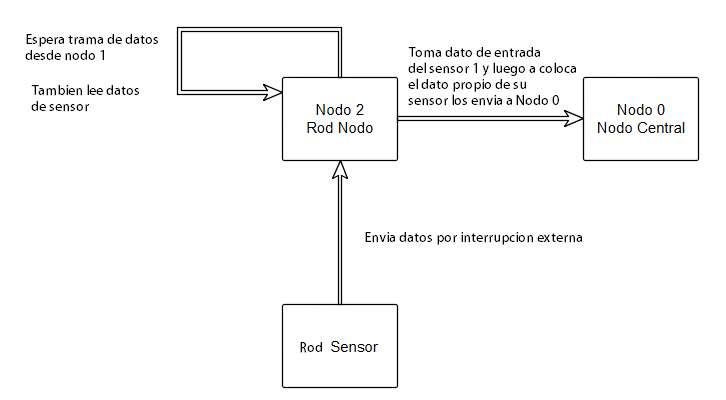
\includegraphics[scale=0.6]{nodo2}
	\caption{M'aquina de estado del Nodo 2}
	\label{fig:nodo2}
\end{figure}

\subsubsection{Programaci'on nodo 2}

Para el envio de datos se hace direccionamiento indirecto de datos; se crean dos variables de clase CAN para guardar el dato de entrada y luego ponerlo en el buffer de salida.
{\tiny
\begin{lstlisting}[language=C]

#include <SPI.h>
#include "mcpointer-can.h"
#include <Encoder.h>
Encoder myEnc(5, 6);
// the cs pin of the version after v1.1 is default to D9
// v0.9b and v1.0 is default D10
const int SPI_CS_PIN = 10;
const int LED=8;
unsigned char len = 0;
unsigned char buf[8]= {0,0,0,0,0,0,0,0};
float   float0=0;
unsigned char *pointer-float0 = (unsigned char *)&float0;
int   aux=0;
float   aux2=0;
 float u=0;
  float v=0;
   float w=0;
   int z=0;
unsigned char stmp[8] = {0, 0, 0, 0, 0, 0, 0, 0};

float   float10=0; //keep the data from the arduino w sensor 1
float *pointer-float10 = (float *)&buf[0]; //value

MCpointer-CAN CAN(SPI_CS_PIN);                                    // Set CS pin

void setup()
{
    Serial.begin(115200);
    pinMode(LED,OUTPUT);

    while (CAN_OK != CAN.begin(CAN_1000KBPS))              // init can bus : baudrate = 500k
    {
        //Serial.println("CAN BUS Shield init fail");
     //   Serial.println(" Init CAN BUS Shield again");
      }
    //Serial.println("CAN BUS Shield init ok!");
}
void loop()
{
  float0=  myEnc.read(); 
  read();  
}

void read(){
    if(CAN_MSGAVAIL == CAN.checkReceive())            // check if data coming
    {
      CAN.readMsgBuf(&len, buf);    // read data,  len: data length, buf: data buf
      unsigned char canId = CAN.getCanId();
       //Serial.println(CAN.getCanId());
      if(CAN.getCanId()==0x60){
           
        float10=(*pointer-float10);
       
        Serial.println(float0);
         
        // v=(buf[0]+(buf[1]*3.917647)/1000);
         //u=(buf[2]*3.917647)/1000;
         //z=v*100;
        //w=(1.00*z/100)+((u/100));
        //w=v+((u/1000));
        stmp[0]= buf[0];
        stmp[1]= buf[1];
        stmp[2]= buf[2];
        stmp[3]= buf[3];
        //stmp[3]= float0;
        stmp[4]= pointer-float0[0];
        stmp[5]= pointer-float0[1];
        stmp[6]= pointer-float0[2];
        stmp[7]= pointer-float0[3];
        CAN.sendMsgBuf(0x20,0, 8, stmp);  
        
            digitalWrite(LED,1);
       
    }           
    digitalWrite(LED,1);
  }  
  }

\end{lstlisting}
}
\subsubsection{Sistema el'ectrico del nodo 2}

La Fig. \ref{fig:nodo1electric}, muestra la conexi'on a utilizarse en el nodo 2, la cual es similar al nodo 1.
\subsection{Dise'no l'ogico de la estructura de la red: Nodo 3}
\subsubsection{M'aquina de estados del Nodo 3}
\begin{figure}[ht]
	\centering
		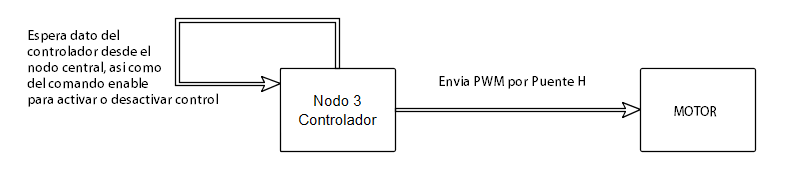
\includegraphics[scale=0.65]{nodo3}
	\caption{M'aquina de estados del Nodo 3}
	\label{fig:nodo3}
\end{figure}

\subsubsection{Nodo del motor: Nodo 3 }
En este nodo se pone en evidencia las acciones enviadas por el controlador central (Fig. \ref{fig:nodo3}).

\subsubsection{Programaci'on nodo 3}

{\tiny
\begin{lstlisting}[language=C]

#include <SPI.h>
#include "mcpointer-can.h"

// the cs pin of the version after v1.1 is default to D9
// v0.9b and v1.0 is default D10
const int SPI_CS_PIN = 10;
const int LED=8;
float   aux2=0;
boolean ledON=1;
unsigned char stmp[8] = {0, 0, 0, 0, 0, 0, 0, 0};
MCpointer-CAN CAN(SPI_CS_PIN);                                    // Set CS pin

void setup()
{
    Serial.begin(115200);
    pinMode(LED,OUTPUT);

    while (CAN_OK != CAN.begin(CAN_1000KBPS))              // init can bus : baudrate = 500k
    {
        Serial.println("CAN BUS Shield init fail");
        Serial.println(" Init CAN BUS Shield again");
        
    }
    Serial.println("CAN BUS Shield init ok!");
}
void loop()
{
  read();   
}

void read(){
  unsigned char len = 0;
    unsigned char buf[8];

    if(CAN_MSGAVAIL == CAN.checkReceive())            // check if data coming
    {
      CAN.readMsgBuf(&len, buf);    // read data,  len: data length, buf: data buf
      unsigned char canId = CAN.getCanId();
       //Serial.println(CAN.getCanId());
      if(CAN.getCanId()==0x10){

        Serial.println("-----------------------------");
        Serial.println("get data from ID: ");
        Serial.println(canId);

        for(int i = 0; i<len; i++)    // print the data
        {
            Serial.print(buf[i]);
            Serial.print("\t");
            
             if(!buf[0])
            {

                digitalWrite(LED,1);
                ledON=1;
            }
        }
        Serial.println();     
    }           
  }
  }

/*********************************************************************************************************
  END FILE
*********************************************************************************************************/
 \end{lstlisting}
}


\subsubsection{Sistema esquem'atico el'ectrico del nodo 3}

A continuaci'on se detalla el sistema de conexi'on del sistema el'ectrico del nodo 0 en la Fig. \ref{fig:nodo3electric}:

\begin{center}
\begin{figure}[ht]
	\centering
		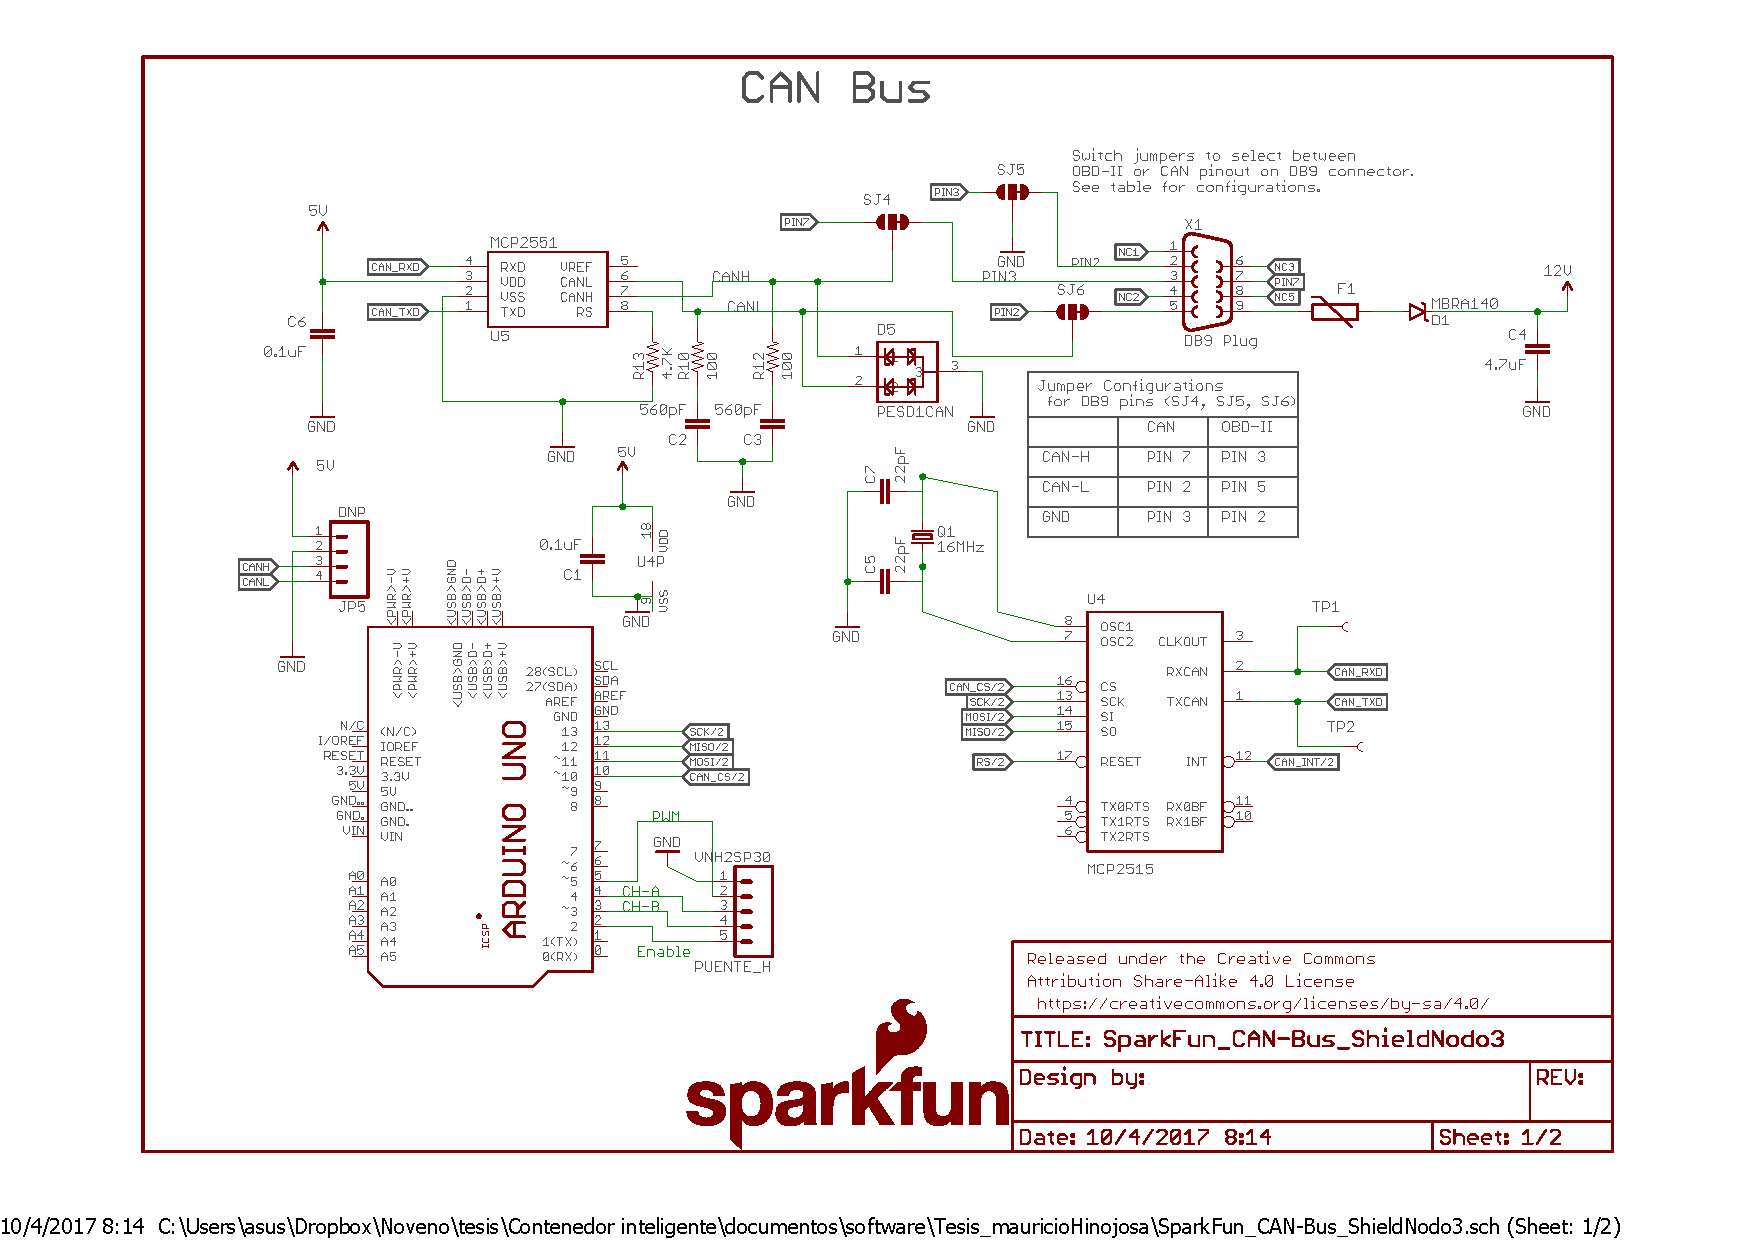
\includegraphics[width=14cm, height=10cm]{nodo3e}
	\caption{Diagrama el'ectrico del nodo 3}
	\label{fig:nodo3electric}
\end{figure}
\end{center}

\subsection{Red f'isica CAN e interconexi'on con la HMI}

En esta secci'on se muestra la interconexi'on de la red CAN y la HMI, as'i como de los sensores implementados en la red; el puente H de electr'onica del sistema como se muestra en la Fig.\ref{fig:canhmi}.
\begin{center}
\begin{figure}[ht]
	\centering
		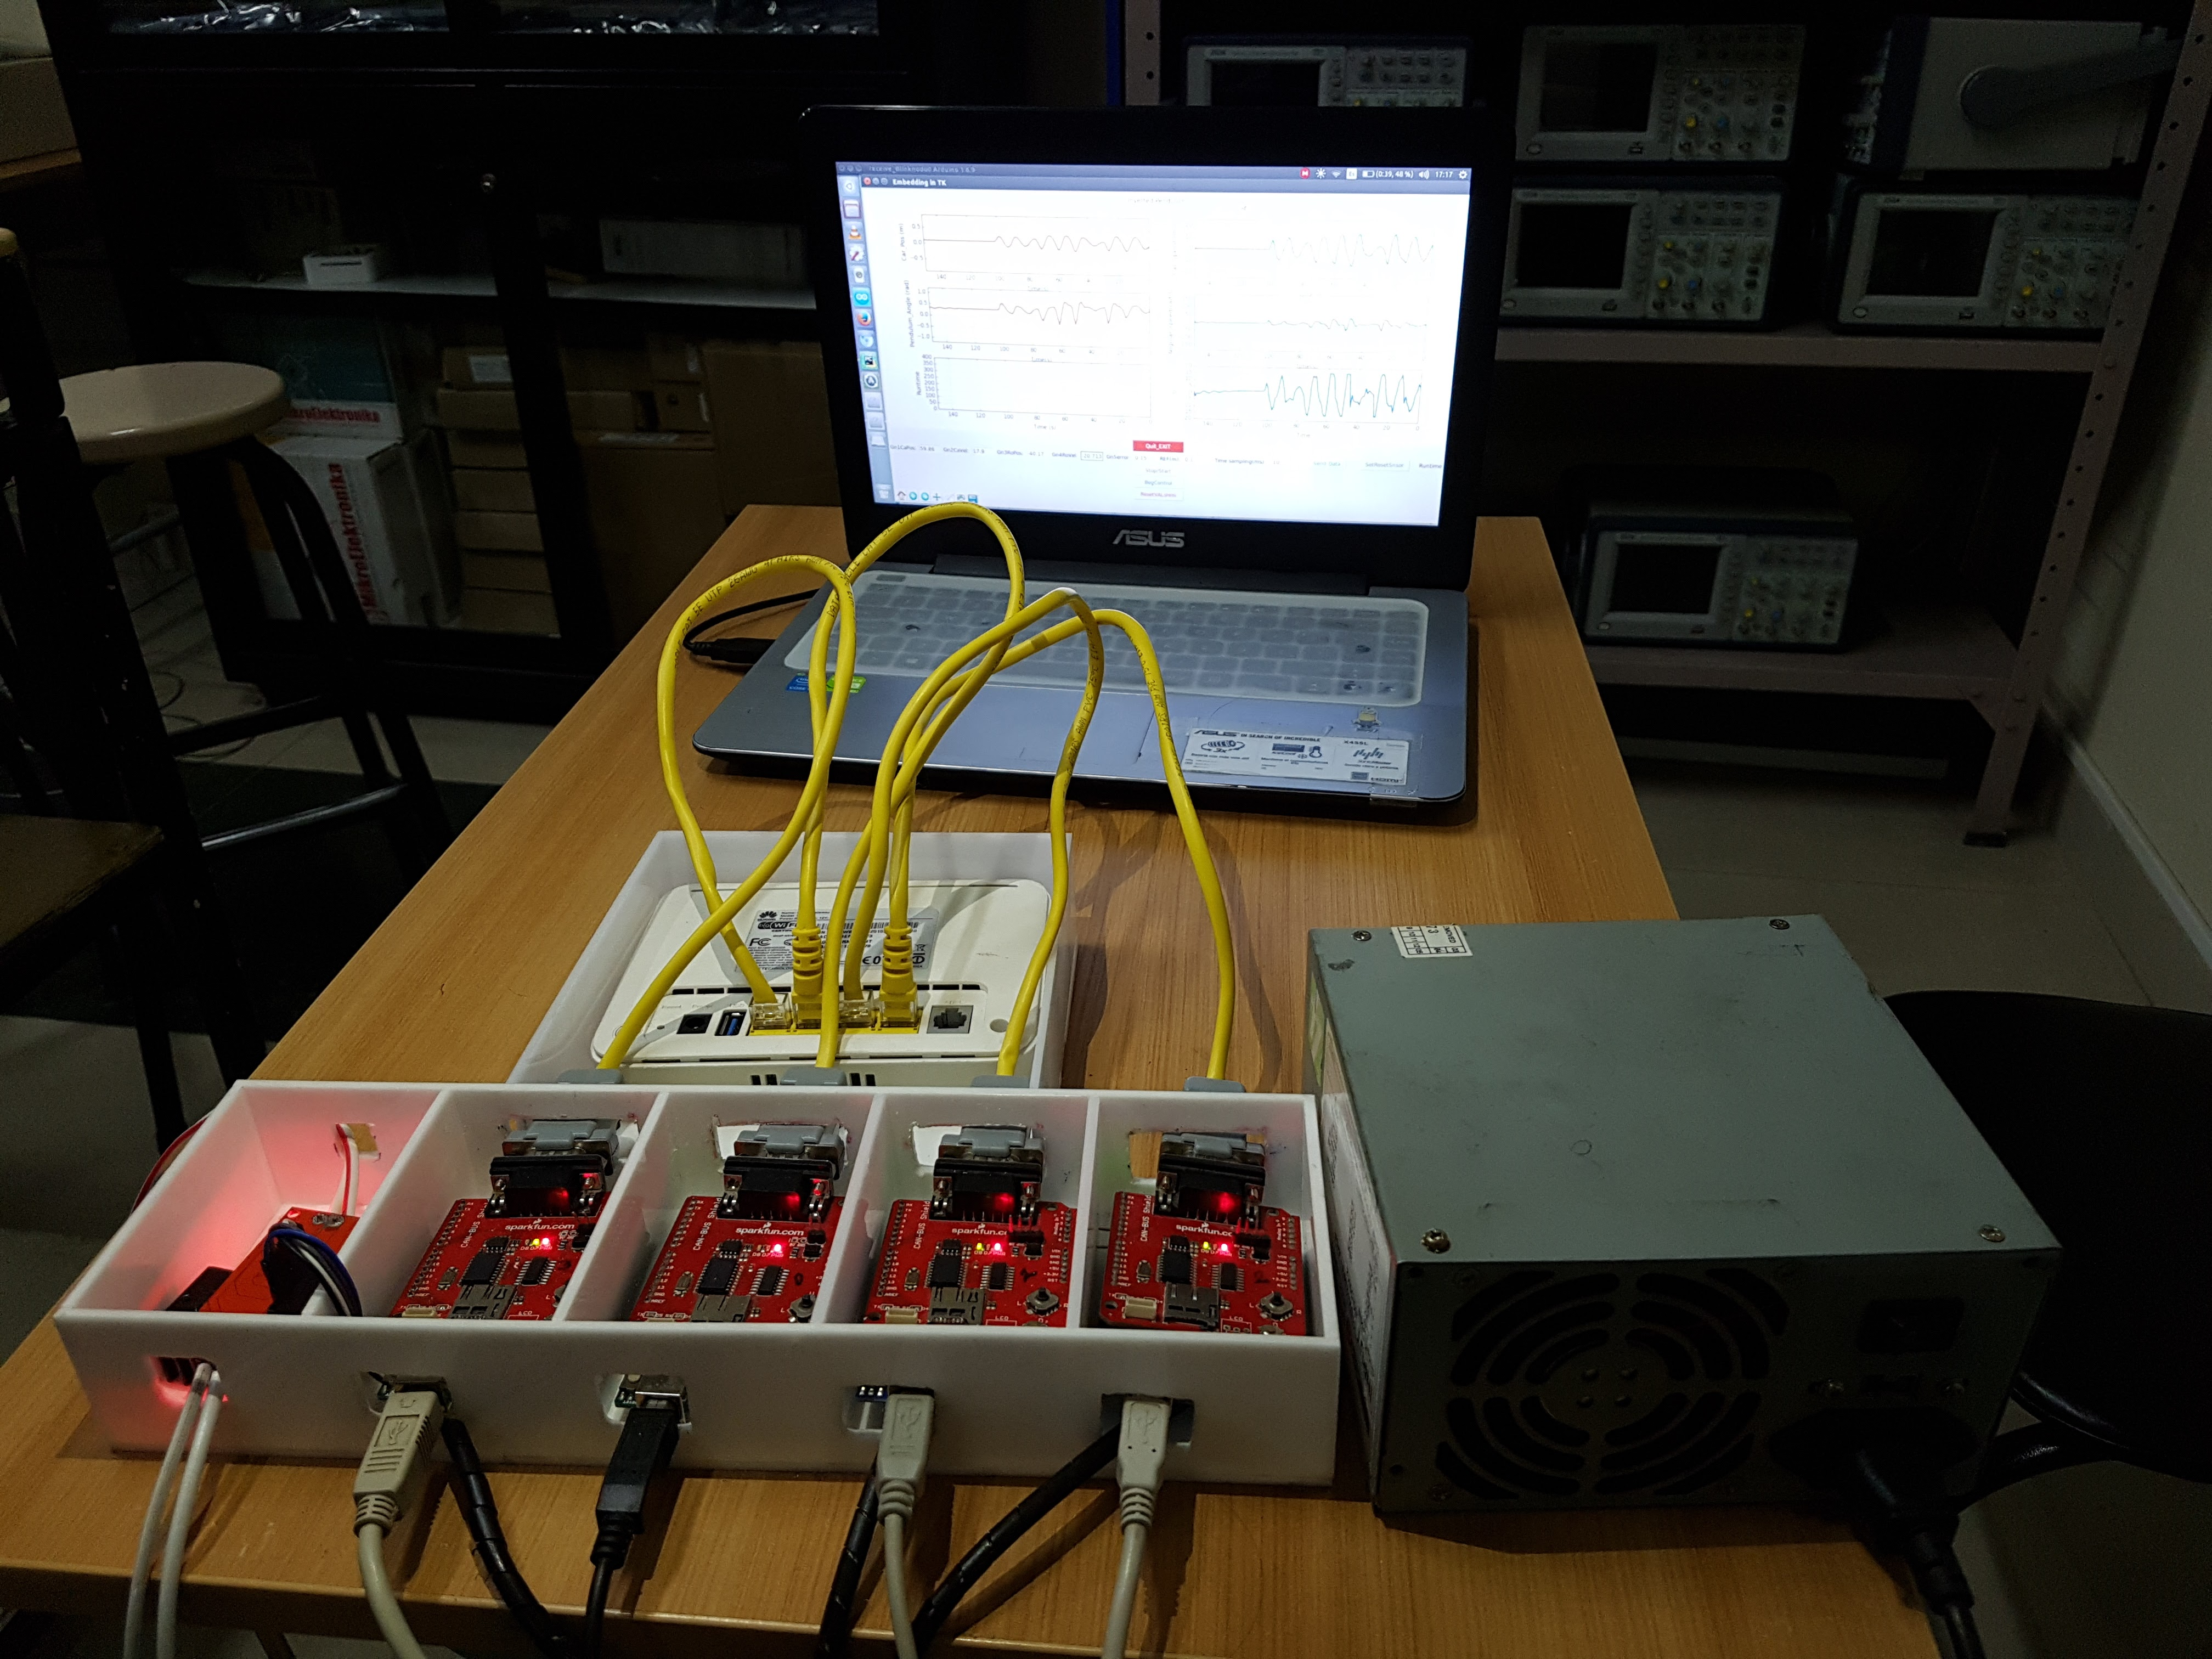
\includegraphics[width=14cm, height=10cm]{canhmi}
	\caption{CAN y HMI}
	\label{fig:canhmi}
\end{figure}
\end{center}


\section{Dise'no de la HMI}
\subsection{Instalaci'on de Python en Ubuntu}
La instalaci'on de Python dentro de Ubuntu no tiene ninguna complicaci'on:
\begin{itemize}
	\item Se debe abrir una terminal \textbf{(Ctrl $+$ Alt $+$ t)}.
	\item Con la correspondiente conexi'on a internet y  se debe escribir en consola lo siguiente:
	
	\begin{itemize}
		\item {\small
\begin{lstlisting}[language=C]
sudo add-apt-repository ppa:fkrull/deadsnakes
\end{lstlisting}
}

		\item {\small
\begin{lstlisting}[language=C]
sudo apt-get update
\end{lstlisting}
}
		\item {\small
\begin{lstlisting}[language=C]
sudo apt-get install python2.7
\end{lstlisting}
}
	\end{itemize}
	\item Por ultimo: {\small\begin{lstlisting}[language=C]
	sudo apt-get update \end{lstlisting}}
	{\small\begin{lstlisting}[language=C]
	sudo apt-get upgrade \end{lstlisting}} y todo estar'a listo para ejecutar Python.
\end{itemize}

\subsection{Instalaci'on de PyCharm}
PyCharm es un IDE, que tiene una version paga y una versi'on (community) de libre de desarrollo la cual ser'a implementada para el desarrollo del sistema HMI, y utiliza como estructructura y lenguaje de desarrollo el antes instalado Python 2.7.2, entre algunos otros lenguajes; y contiene varias herramientas de desarrollo, como ya se explico en secciones anteriores.
La instalaci'on de PyCharm dentro de Ubuntu no tiene ninguna complicaci'on:
\begin{itemize}
	\item Se debe abrir una terminal.
	\item Con la correspondiente conexi'on a internet y escribir en la consola lo siguiente:
	
	\begin{itemize}
		\item {\small
\begin{lstlisting}[language=C]
sudo add-apt-repository ppa:mystic-mirage/pycharm
\end{lstlisting}
}

		\item {\small
\begin{lstlisting}[language=C]
sudo apt-get update
\end{lstlisting}
}
		\item {\small
\begin{lstlisting}[language=C]
sudo apt-get install pycharm-community
\end{lstlisting}
}
	\end{itemize}
	\item Por ultimo se hace un : {\small\begin{lstlisting}[language=C]
	sudo apt-get update \end{lstlisting}}
	{\small\begin{lstlisting}[language=C]
	sudo apt-get upgrade \end{lstlisting}} y todo estar'a listo para ejecutar Python.
\end{itemize}



\subsection{Desarrollo del software}

EL desarrollo del software de supervisi'on de la HMI, parti'o de un software b'asico de intercambio de informaci'on con un Arduino programado en lenguaje \textbf{Python 2.7.2} mostrado en los anexos; en el que el programa se envia dos datos y el arduino respond'ia devolviendo los mismos datos cada cierto tiempo, para graficarlos en la HMI. Basados en esta premisa  se tuvo principalmente tres etapas de desarrollo: expansi'on el buffer del puerto Usb para el env'io de datos, desarrollo de los sistemas gr'aficos y de procesamiento de informaci'on y el desarrollo de controles para el HMI.

\subsection{Expansi'on el buffer del puerto Usb}

Al principio la informaci'on que se enviaba desde la HMI era de un dos datos por el buffer de salida de la HMI; a lo cual se procedi'o a expandirlo hasta que se puedan enviar los datos necesarios para el control desde la HMI final, dando como resultado 10 datos o 40 bytes de informaci'on a la targeta de Arduino que corresponde al nodo 0 o controlador central conectado por Usb a la Pc.


\subsection{Desarrollo de los sistemas gr'aficos y de procesamiento de informaci'on }
Se contaba con una s'ola gr'afica implementada en el programa origen, de la cual se parti'o para conseguir 6 gr'aficas, de las que la primera representa la posici'on del sensor del carro, en la segunda muestra la velocidad de cambio de posici'on del carro; la tercera datos de posici'on del sensor del p'endulo; en la cuarta se regresenta la variaci'on de velocidad del sensor pendular; la quinta el tiempo de procesamiento que lleva el nodo 0 desde su arranque en microsegundos y la sexta representa el controlador.

\subsection{Procesamiento de informaci'on y el desarrollo de controles}

B'asicamente se implentementaron todo tipo de herramientas que permiten desde la creaci'on de botones, cuadros de texto, modificadores gr'aficos  que permiten la manipulaci'on externa de la HMI; hasta la creaci'on de variables que guardan informaci'on o se utilizan para el envio y recepci'on de datos; las clases y objetos que permiten manipular la HMI internamente; librer'ias especiales como la de la Usb o la librer'ia para el empaquetado de datos (todas las librer'ias incluidas en el IDE tool de Python); as'i como como las estructuras l'ogicas o matem'aticas necesarias para el desarrollo; logo de PyCharm en la Fig. \ref{fig:pycharm}
\begin{figure}[ht]
	\centering
		
\includegraphics[scale=0.4]{pycharm}
	\caption{Logo identificativo de Pycharm}
	\label{fig:pycharm}
\end{figure}


\subsection{Programaci'on de la HMI en Python}
A continuaci'on se muestra la programaci'on realizada en Python para la HMI.
\\
 {\tiny
\begin{lstlisting}[language=python]
#!/usr/bin/env python
# -*- coding: utf-8 -*-
"""
@authors: carlos xavier rosero
          manel velasco garc'ia
          Maurico Hinojosa Rea
best performance tested with python 2.7.3, GCC 2.6.3, pyserial 2.5
"""

from __future__ import division
import serial  #serial commun library
import struct  #library to reestructure bytes on buffer
import time #time for delay library
from collections import deque #library for structure of data
import matplotlib
matplotlib.use('TkAgg')
from matplotlib.backends.backend_tkagg import FigureCanvasTkAgg, NavigationToolbar2TkAgg
# implement the default mpl key bindings
from matplotlib.backend_bases import key_press_handler
from matplotlib.pyplot import Figure
import matplotlib.animation as animation #library for plotting
import matplotlib.pyplot as plt #library for plotting
from matplotlib.widgets import Slider, Button, RadioButtons
from Tkinter import *
import sys
if sys.version_info[0] < 3:
    import Tkinter as Tk
else:
    import tkinter as Tk
import os #library native

class puerto:
    puerto0='/dev/ttyACM0'
    j=0
    j=1
    i=0
#########################################
# ###########################################################
##########################################                       ###################################
##########################################  VENTANA DE Puertos ###################################
##########################################                       ###################################
####################################################################################################

class AllTkinterWidgets:
    def __init__(self, master):
        frame = Tk.Frame(master, width=500, height=400, bd=1)
        frame.pack()

        iframe1 = Tk.Frame(frame, bd=2, relief=SUNKEN)

        def closeall():

            master.quit()  # stops mainloop
            master.destroy()
            puerto.j=2

        def closewindow():

            master.quit()  # stops mainloop
            master.destroy()


        def selectbutton():
            puerto.j=1
            k = v.get()
            puerto.puerto0 = k
            print k
            print puerto.puerto0


        Tk.Button(iframe1, text='CloseAll', fg="red",
				command=closeall).pack(side=LEFT, padx=5)
        Tk.Button(iframe1, text='Done', fg="blue",
				command=closewindow).pack(side=LEFT, padx=5)
        Tk.Button(iframe1, text='Select Port',fg="green",
				command=selectbutton).pack(side=LEFT, padx=5)
        #Tk.Checkbutton(iframe1,
				#text='CheckButton').pack(side=LEFT, padx=5)

        v = StringVar()

        a=Tk.Radiobutton(iframe1, text='/dev/ttyACM5', variable=v,
                    value='/dev/ttyACM5').pack(side=RIGHT, anchor=W)
        b=Tk.Radiobutton(iframe1, text='/dev/ttyACM4', variable=v,
                    value='/dev/ttyACM4').pack(side=RIGHT, anchor=W)

        c=Tk.Radiobutton(iframe1, text='/dev/ttyACM3', variable=v,
                    value='/dev/ttyACM3').pack(side=RIGHT, anchor=W)

        d=Tk.Radiobutton(iframe1, text='/dev/ttyACM2', variable=v,
                    value='/dev/ttyACM2').pack(side=RIGHT, anchor=W)

        e=Tk.Radiobutton(iframe1, text='/dev/ttyACM1', variable=v,
                    value='/dev/ttyACM1').pack(side=RIGHT, anchor=W)
        f=Tk.Radiobutton(iframe1, text='/dev/ttyACM0', variable=v,
                       value='/dev/ttyACM0').pack(side=RIGHT, anchor=W)
        iframe1.pack(expand=1, fill=X, pady=10, padx=5)


root = Tk.Tk()
# root.option_add('*font', ('verdana', 10, 'bold'))
all = AllTkinterWidgets(root)
root.title('Port Selection')
root.mainloop()

#########################################
# ###########################################################
##########################################                       ###################################
##########################################  VENTANA DE MONITOREO ###################################
##########################################                       ###################################
####################################################################################################

class command:
    startCx = 0xf0  #startcx value for comunication
    startCx2 = 0xf2  #startcx value for comunication 2
    stopCx = 0xf1   #stopcx value for comunication


class cons:

    #######################################
    ###### here we create global variables#####
    #######################################

    div=1
    max1=0
    runtime1=float(0)
    k=float(0)
    ts=float(50)
    onoff=float(1)
    typecontroll=float(1)





# use this part only with old versions of python and libraries
# tested specifically with python 2.6.5, GCC 4.4.3, serial 1.3.5
class adapt(serial.Serial):
    def write(self, data):
        super(self.__class__, self).write(str(data))

#################################################

class serialCx:

    def __init__(self, usbPort, frameLen, maxLen, EOL, bauds):
        #SELF (VARIABLES for the _init_ class)
        self.ay1 = deque([0.0] * maxLen)
        self.ay2 = deque([0.0] * maxLen)
        self.ay3 = deque([0.0] * maxLen)
        self.ay4 = deque([0.0] * maxLen)
        self.ay5 = deque([0.0] * maxLen)
        self.maxLen = maxLen
        self.eol = EOL  # end of line
        self.lenEol = len(self.eol)  # length of the end of line
        self.frameLen = frameLen - self.lenEol
        self.float0 = float(0) #var analog1
        self.float1 = float(0) #var analog2
        self.valor1 = float(0) #var analog1 dy/dt
        self.valor2 = float(0) #var analog2 dy/dt
        self.runtime = float(0)  # var analog2 dy/dt
                            #this all var are going to the plot
        # open serial port
        self.ser = adapt(port=usbPort,
				baudrate=bauds, timeout=1, parity=serial.PARITY_NONE,
                         stopbits=serial.STOPBITS_ONE)

        #######################################
        ######here we send initial values to the arduino0 #####
        #######################################

        #self.ser.open
        #self.ser.isOpen
        time.sleep(2)  # waits until arduino gets up
        inputS = []  # initializes buffer
        while self.ser.inWaiting() > 0:  # neglects the trash code received
            inputS.append(self.ser.read(1))  # appends a new value into the buffer

        self.float0ToTx = cons.k  # initial values of the floating
				#numbers to be sent--------> value of k gain
        self.float1ToTx = cons.ts # initial values of the floating
				#numbers to be sent--------> value of ts (tme sampling) 10-50 ms
        self.float2ToTx = cons.onoff  # initial values of the floating 
				#numbers to be sent--------> on/of arduino's communication
        self.float3ToTx = cons.typecontroll  # initial values of the floating 
				#numbers to be sent--------> Tipe of controller crank/inverted

        cons.div=self.float1ToTx
        value0 = struct.pack('%sf' % 1, self.float0ToTx)  # splits the float value into 4 strings
        value1 = struct.pack('%sf' % 1, self.float1ToTx)  # splits the float value into 4 strings
        value2 = struct.pack('%sf' % 1, self.float2ToTx)  # splits the float value into 4 strings
        value3 = struct.pack('%sf' % 1, self.float3ToTx)  # splits the float value into 4 strings

        time.sleep(0.2) #this wait before buffer finish write
        # this buffer sends the command to start tx from arduino and both floating registers
        buffer = bytearray([command.startCx,
				ord(value0[0]), ord(value0[1]), ord(value0[2]), ord(value0[3]),
        ord(value1[0]), ord(value1[1]), ord(value1[2]), ord(value1[3])])

        self.ser.write(buffer)  # sends the command to start the reception

        time.sleep(0.075) #this wait before buffer finish write

        buffer = bytearray([command.startCx2,
				ord(value2[0]), ord(value2[1]), ord(value2[2]), ord(value2[3]),
        ord(value3[0]), ord(value3[1]), ord(value3[2]), ord(value3[3])])
        self.ser.write(buffer)  # sends the command to start the reception
        # add to buffer
        time.sleep(0.1)  # this wait before buffer finish write


    def addToBuf(self, buf, val):
        if len(buf) < self.maxLen:
            buf.append(val)
        else:
            buf.pop()
            buf.appendleft(val)


    # update plot
    def update(self, frameNum, a1, a2, a3, a4,rtime):

        #######################################
        ######here we get the data from the buffer for update on plots #####
        #######################################

        line = bytearray()
        try:
            while True:
                c = self.ser.read(1)
                if c:
                    line.append(c)
                    if line[-self.lenEol:] == self.eol:  # verifies if EOF has been received
                        line = line[0:-self.lenEol]  # removes EOF
                        break
                else:
                    break

            if len(line) == self.frameLen:
                self.float0 = struct.unpack('f', line[0:4])
                self.float0 = self.float0[0]  # takes out the only one element from the tuple
                self.float1 = struct.unpack('f', line[4:8])
                self.float1 = self.float1[0]  # takes out the only one element from the tuple
                self.valor1 = struct.unpack('f', line[8:12])
                self.valor1=self.valor1[0]   # takes out the only one element from the tuple
                self.valor2 = struct.unpack('f', line[12:16])
                self.valor2 = self.valor2[0]  # takes out the only one element from the tuple
                self.runtime = struct.unpack('f', line[16:20])
                self.runtime = self.runtime[0]   # takes out the only one element from the tuple

                print self.float0, #coma ad a espace on the plot window
                print self.float1,
                print self.valor1,
                print self.valor2,
                print self.runtime,
                print cons.ts,
                print cons.k,
                print cons.onoff,
                print cons.typecontroll
                cons.max1 = self.valor1
                cons.runtime1=self.runtime

                # add data to buffer
                self.addToBuf(self.ay1, self.float0)
                self.addToBuf(self.ay2, self.float1)
                self.addToBuf(self.ay3, self.valor1)
                self.addToBuf(self.ay4, self.valor2)
                self.addToBuf(self.ay5, self.runtime)
                a1.set_data(range(self.maxLen), self.ay1)
                a2.set_data(range(self.maxLen), self.ay2)
                a3.set_data(range(self.maxLen), self.ay3)
                a4.set_data(range(self.maxLen), self.ay4)
                rtime.set_data(range(self.maxLen), self.ay5)
            else:
                print 'Incorrect frame length:',
                print self.float0,  # coma ad a espace on the plot window
                print self.float1,
                print self.valor1,
                print self.valor2,
                print self.runtime
                print self.frameLen
                print len(line)
                #self.ser.write(buffer)
                #self.ser.flushInput()  # gets empty the serial port buffer


        except KeyboardInterrupt:
            print('Exiting...')

    def printrtime(self):
        print self.runtime
        return self.runtime
    # clean up
    def close(self):
        # close serial

        buffer = bytearray([command.stopCx, 0x01, 0x01, 0x01, 0x01, 0x01, 0x01,
                            0x01, 0x01])  # the (0x01) is used only to fill the buffer
        # in order to accomplish the standard length

        self.ser.write(buffer)  # sends the command to start the reception

        self.ser.flushInput()
        self.ser.close()




def plotting(givenData):


    #######################################
    ###### here we create the variables for canvas and plt #####
    #######################################

    root = Tk.Tk()
    root.wm_title("Embedding in TK")
    #f = plt.figure(figsize=(9, 6), dpi=95, facecolor = 'w', edgecolor = 'k')
    fig = plt.figure(num = 1, figsize = (9, 5.5),
		dpi = 95, facecolor = 'w', edgecolor = 'k') #modifie plot's properties


    #######################################
    ######this are just propierties of plt and sub plt#####
    #######################################

    plt.rc('lines', linewidth=1.2) #modifie weigh of lines
    plt.rc('font', size=10) # modifie weight of text
    plt.suptitle('Inverted Pendulum')# add subplot title
    plt.subplots_adjust(hspace=0.30)



    #######################################
    ###### here we can change properties from each subplots #####
    #######################################

    #ax1 =  f.add_subplot(111)
    ax1 = plt.subplot(321)
    ax1.grid(True)
    a1, = ax1.plot([0], [0], color=(0, 1, 1)) ##comma means continuous plotting
    plt.xlim(0, 150)
    plt.ylim(-2500, 2500)

    plt.xlim(plt.xlim()[::-1])
    plt.ylabel('Analog1')
    plt.xlabel('Time')
    plt.grid(color = 'r', linewidth = 1)
    #plt.legend(loc=2)
    plt.title('', fontsize=20, color='0.5', verticalalignment=
		'baseline', horizontalalignment='center')

    ax2 = plt.subplot(323)
    ax2.grid(True)
    a2, = ax2.plot([0], [0], color=(1, 1, 0))
    plt.xlim(0, 150)
    plt.ylim(-2500, 2500)
    plt.xlim(plt.xlim()[::-1])#invert x axe's direction if
		#this line is disable plotting change direction
    plt.ylabel('Analog2')
    plt.xlabel('Time')
    plt.grid(color = 'b', linewidth = 1)
    plt.title(' ', fontsize=20, color='0.5', verticalalignment='baseline', 
		horizontalalignment='center')

    ax3 = plt.subplot(322)
    ax3.grid(True)
    a3, = ax3.plot([0], [0], color=(0, 1, 0))
    plt.xlim(0, 15)
    plt.ylim(-50, 50)  # modifie limits on y axis
    plt.xlim(plt.xlim()[::-1])  # invert x axe's direction
    plt.ylabel('Derivative1')
    plt.xlabel('Time')
    plt.grid(color='m', linewidth=1)
    plt.title(' ', fontsize=20, color='0.5', verticalalignment='baseline', 
		horizontalalignment='center')

    ax4 = plt.subplot(324) #_first num add y subplots _second_num add
		#x subplot _3_num put in the correct place the subplot
    ax4.grid(True)#this add grid on subplot
    a4, = ax4.plot([0], [0], color=(0, 0, 1)) #
    #a3, = ax4.plot([0], [0], color=(0, 1, 0)) #unline to plot two lines in the same plot
    plt.xlim(0, 15) #modifie limits on x axis
    plt.ylim(-50, 50) #modifie limits on y axis
    plt.xlim(plt.xlim()[::1])  # invert x axe's direction

    plt.ylabel('Derivative2') #this add ylabel title
    plt.xlabel('Time') #this add xlabel title
    plt.grid(color='y', linewidth=1) #modifie properties of the grid
    plt.title(' ', fontsize=20, color='0.5', 
		verticalalignment='baseline', horizontalalignment=
		'center')#modifie title's properties on subplots

    ax5 = plt.subplot(325) #_first num add y subplots _second_num add 
		#x subplot _3_num put in the correct place the subplot
    ax5.grid(True)#this add grid on subplot
    rtime, = ax5.plot([0], [0], color=(0, 0, 1)) #

    plt.xlim(0, 50) #modifie limits on x axis
    plt.ylim(0, 100000) #modifie limits on y axis
    plt.xlim(plt.xlim()[::-1])  # invert x axe's direction
    plt.ylabel('runtime') #this add ylabel title
    plt.xlabel('Time') #this add xlabel title
    plt.grid(color='g', linewidth=1) #modifie properties of the grid
    plt.title(' ', fontsize=20, color='0.5',
		verticalalignment='baseline', horizontalalignment=
		'center')#modifie title's properties on subplots
    plt.subplots_adjust(left=0.1)
    plt.subplots_adjust(right=0.95)
   # selection2 = str(cons.runtime1)
   # label3.config(text=selection2)
    #anim = animation.FuncAnimation(f, 
		givenData.update, fargs=(a1, a2, a3, a4, rtime),frames=1000, interval=1) 
		#update values on plot #200 frames each 1 ms

    anim = animation.FuncAnimation(fig,
		givenData.update, fargs=(a1, a2, a3, a4, rtime), frames=1000,interval=1)  
		# update values on plot #200 frames each 1 ms

    #######################################
    ######bottons inside canvas #####
    #######################################


    #here we made the canvas for the bottons and other things
    ###############################################
    canvas = FigureCanvasTkAgg(fig, master=root)
    canvas.show()
    canvas.get_tk_widget().pack(side=Tk.TOP, fill=Tk.BOTH, expand=1)

    toolbar = NavigationToolbar2TkAgg(canvas, root)
    toolbar.update()
    canvas._tkcanvas.pack(side=Tk.TOP, fill=Tk.BOTH, expand=1)

    def on_key_event(event):
        print('you pressed %s' % event.key)
        key_press_handler(event, canvas, toolbar)

    canvas.mpl_connect('key_press_event', on_key_event)

    def _quit():
        root.quit()  # stops mainloop
        root.destroy()  # this is necessary on Windows to prevent
        # Fatal Python Error: PyEval_RestoreThread: NULL tstate
    def reset():
         cons.runtime1 = float(0)
         cons.k = float(0)
         cons.ts = float(50)
         cons.onoff = float(1)
         cons.typecontroll = float(1)
         print cons.runtime1,cons.typecontroll,cons.onoff, cons.ts, cons.k
         serialCx(puerto.puerto0, 24, 300, 'cXrC',
                     115200)# Fatal Python Error: PyEval_RestoreThread: NULL tstate

    buttonreset = Tk.Button(master=root, text='Reset', command=reset,fg="red",width=14)
    buttonreset.pack(side=Tk.BOTTOM)
    button = Tk.Button(master=root, text='Quit', command=_quit, fg="red", width=14)
    button.pack(side=Tk.TOP)

    label = Tk.Label(master=root, text="                   ")
    label.pack(side=Tk.LEFT, padx=4)

    labelgain = Tk.Label(master=root, text="Gain : (x.xx)")
    labelgain.pack(side=Tk.LEFT,padx=4)
    e = Tk.Entry(master=root,width=10)
    e.insert(0,0)
    e.pack(side=Tk.LEFT,padx=20)
    e.focus_set()
    labelts = Tk.Label(master=root, text="Time sampling : (x)")
    labelts.pack(side=Tk.LEFT,padx=4)
    f = Tk.Entry(master=root,width=10)
    f.insert(0,10)
    f.pack(side=Tk.LEFT,padx=35)

    #e.focus_set()

    label = Tk.Label(master=root, text="        ")
    label.pack(side=Tk.LEFT)


    def selectcontrolbutton():
        cons.typecontroll = v.get()
        print v.get()
        print cons.typecontroll

    buttoncontrol = Tk.Button(master=root, text='Type Control',
		command=selectcontrolbutton, fg="purple", width=14)
    buttoncontrol.pack(side=Tk.LEFT)
    rootframe=Tk.Frame(root, bd=1, relief=SUNKEN)
    v = IntVar()
    c = Tk.Radiobutton(rootframe, text='Control1', variable=v,
                       value=1).pack(side=TOP)
    d = Tk.Radiobutton(rootframe, text='Control2', variable=v,
                       value=2).pack(side=TOP)
    t = Tk.Radiobutton(rootframe, text='Control3', variable=v,
                       value=3).pack(side=TOP)
    r = Tk.Radiobutton(rootframe, text='Control4', variable=v,
                       value=4).pack(side=TOP)

    rootframe.pack(side=Tk.LEFT,fill=X)

    label = Tk.Label(master=root, text="          ")
    label.pack(side=Tk.LEFT)



    def changevalbutton():
        k = e.get()
        l = f.get()
        cons.k=float(k)
        cons.ts = int(l)
        print k,l,cons.ts,cons.k
        serialCx(puerto.puerto0, 24, 300, 'cXrC',
                                115200)  # This values modifie serialport, 
		  	#Length of bytes in tx,Length of data plotting, and bauds
        print k, l, cons.ts, cons.k


    def stopcanbutton():

        if puerto.i==1:
            cons.onoff=1
            puerto.i=0
        else:
            cons.onoff = 0
            puerto.i = 1
        print cons.onoff
        serialCx(puerto.puerto0, 24, 300,
				        'cXrC',
                 115200) 
			# This values modifie serialport, 
      #Length of bytes in tx,Length of data plotting, and bauds

        print cons.onoff
        print puerto.i

    b3 = Tk.Button(master=root, text="Send Data", command=changevalbutton, fg="green")
    b3.pack(side=Tk.LEFT,pady=10,padx=10)

    label = Tk.Label(master=root, text="          ")
    label.pack(side=Tk.LEFT)

    b4 = Tk.Button(master=root, text="Stop/Start CAN COM", command=stopcanbutton)
    b4.pack(side=Tk.BOTTOM, pady=10)


    labelruntime = Tk.Label(master=root,text="Runtime")
    labelruntime.pack(side=Tk.LEFT,pady=10)
    label = Tk.Label(master=root, text="    ")
    label.pack(side=Tk.LEFT)
    def runtimebutton():
        s = cons.runtime1
        labelruntime.config(text=s)

    b2 = Tk.Button(master=root, text="Runtime", command=runtimebutton, fg="blue")
    b2.pack(side=Tk.LEFT,pady=10)
    label = Tk.Label(master=root, text="      ")
    label.pack(side=Tk.LEFT)

    #    b2 = Tk.Button(master=root, text="runtime", command=runtimebutton)
 #   b2.pack(side=Tk.RIGHT)




    #######################################
    ######update data from plt from pyplot#####
    #######################################

    #here the plt or figure is updating
    anim = animation.FuncAnimation(fig, givenData.update, fargs=(a1, a2, a3, a4, rtime), frames=1000,
                                   interval=1)  # update values on plot #200 frames each 1 ms
    #plt.show()
    Tk.mainloop()


   # plt.close()
    #plt.show()

    #Tk.mainloop()


#######################################
######here starts the main program#####
#######################################


if __name__ == "__main__":

    testMauricio = serialCx(puerto.puerto0, 24, 300, 'cXrC', 115200) #This values modifie serialport, 
		#Length of bytes in tx,Length of data plotting, and bauds
    if puerto.j==1:
        plotting(testMauricio) #plotting
    serialCx.close(testMauricio) #close all process


\end{lstlisting}

}


\subsection{Ventana HMI terminada}

Concluida la programaci'on se tienen dos ventanas; la primera es una peque'na ventana que permite seleccionar entre diferentes puertos Usb, posibles en Ubuntu  como muestra la Fig. \ref{fig:usb}.
\begin{figure}[ht]
	\centering
		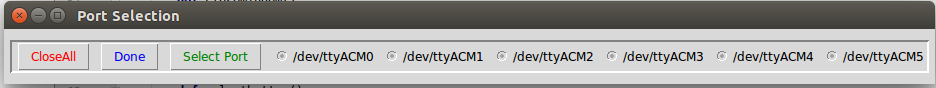
\includegraphics[scale=0.6]{usb}
	\caption{Ventana de selecci'on Usb}
	\label{fig:usb}
\end{figure}
\begin{figure}[ht]
	\centering
		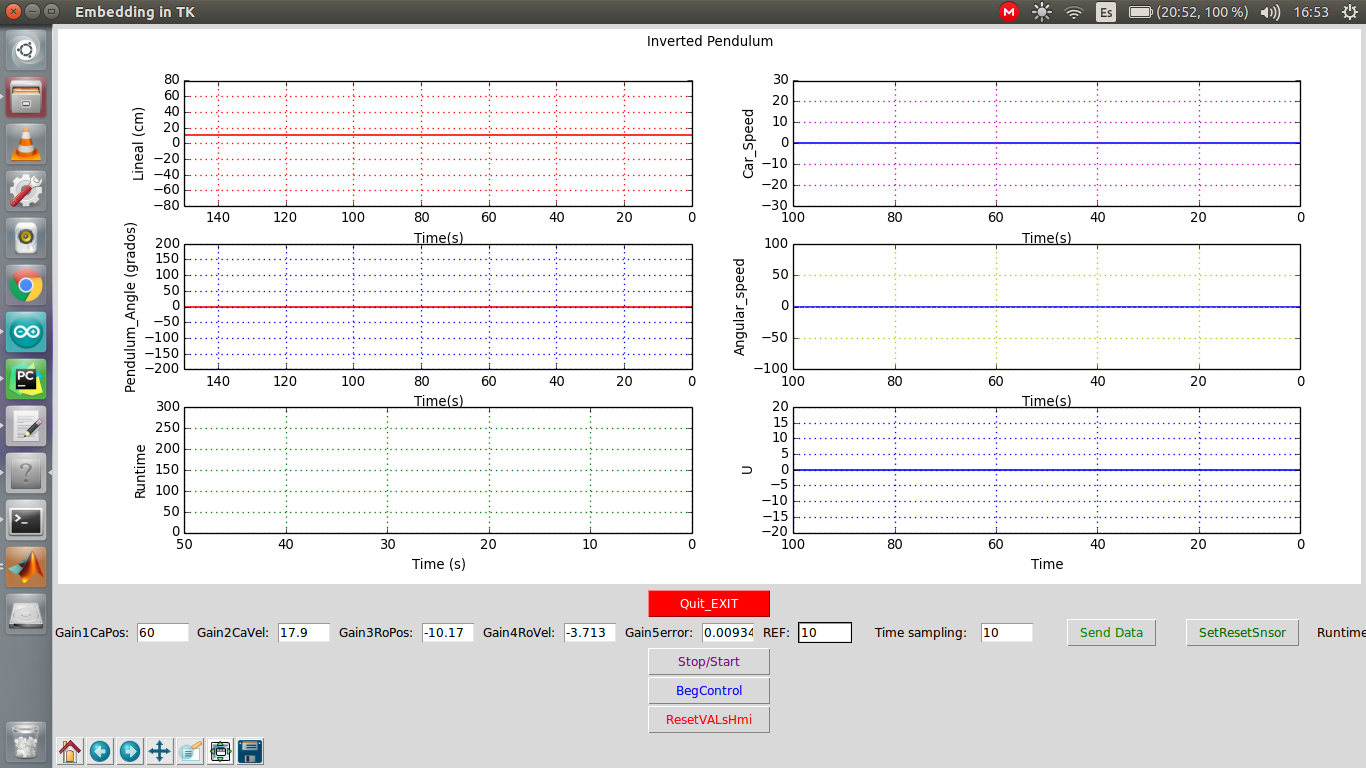
\includegraphics[scale=0.45]{HMI}
	\caption{HMI}
	\label{fig:HMI}
\end{figure}

La segunda ventana es la HMI utilizar en el sistema como muestra Fig. \ref{fig:HMI}, consta de las partes:

\begin{enumerate}
	\item Gr'afica sensor 1.
	\item Gr'afica de la variaci'on de velocidad sensor 1.
	\item Gr'afica sensor 2.
	\item Gr'afica de la variaci'on de velocidad sensor 2.
	\item Gr'afica del tiempo de procesamiento en microsegundos.
	\item Botones y texto de informaci'on y modificaci'on de los valores de control del p'endulo.
	\item Barra de manipulaci'on de las gr'aficas.
\end{enumerate}


\section{Tr'amas de datos enviados desde HMI hacia el nodo central}

Esta es la trama de datos enviado por la HMI hacia el nodo central:\\

{\small
\lstset{language=python, breaklines=true}
\begin{lstlisting}[frame=single]
([command.direccion, ord(value0[0]), ord(value0[1]), ord(value0[2]), ord(value0[3]),
        ord(value1[0]), ord(value1[1]), ord(value1[2]), ord(value1[3]),
        ord(value2[0]), ord(value2[1]), ord(value2[2]), ord(value2[3]),                             
        ord(value3[0]), ord(value3[1]), ord(value3[2]), ord(value3[3]),
        ord(value4[0]), ord(value4[1]), ord(value4[2]), ord(value4[3]),
        ord(value5[0]), ord(value5[1]), ord(value5[2]), ord(value5[3]),
        ord(value6[0]), ord(value6[1]), ord(value6[2]), ord(value6[3]),
        ord(value7[0]), ord(value7[1]), ord(value7[2]), ord(value7[3]),
        ord(value8[0]), ord(value8[1]), ord(value8[2]), ord(value8[3]),
        ord(value9[0]), ord(value9[1]), ord(value9[2]), ord(value9[3]),0x0A])                                

\end{lstlisting}
}
Contiene 42 bytes estructurados en una sola trama de datos que controla el sistema en los nodos arduinos.\\
\\
   Donde: value0= estructura en 4 bytes el valor de la ganancia G1.\\
					value1= estructura en 4 bytes el valor de time sampling.\\
					value2= estructura en 4 bytes el valor del \textit{on/off} del sistema de comunicaci'on.\\
					value3= estructura en 4 bytes el valor del reset de sensores.\\
					value4= estructura en 4 bytes el valor de la ganancia G2.\\
					value5= estructura en 4 bytes el valor de la ganancia G3.\\
					value6= estructura en 4 bytes el valor de la ganancia G4.\\
					value7= estructura en 4 bytes el valor de la ganancia G5.\\
					value8= estructura en 4 bytes el valor de la referencia.\\
					value9= estructura en 4 bytes el valor de enable del control (enciende o paga el controlador).
					
	El valor de \textit{\textbf{command.direccion}} permite seleccionar las acciones en los nodos:
	
	\begin{itemize}
		\item  Si command.direccion =0xf1 entonces se apagan y cierran comunicaciones con HMI.
		\item  Si command.direccion =0xf0 entonces se detienen o reinician comunicaciones con HMI.
		\item  Si command.direccion =0xf2 entonces se recepcionan ganancias variables para el controlador.
		\item  Si command.direccion =0xf3 entonces se activa o desactiva el controlador.
		\item  Si command.direccion =0xf4 entonces se resetean valores tanto en nodo central como en HMI.
		\item  Si command.direccion =0xf5 entonces se envia mensaje para resetear sensores.
		
		
	\end{itemize}
	
	El 'ultimo valor (0x0A) es estandar para final de trama.

\section{Tr'amas de datos enviados y recibidas entre nodos}

\subsection{Nodo 0}
En la secci'on anterior se mostr'o la trama de datos enviada desde la HMI hacia el nodo central (nodo0).

\subsection{Nodo 0 a HMI}
La siguiente trama \ref{tabla:ncHMI} de datos representa los bytes enviados desde el nodo central hacia la HMI.

\begin{table}[htbp]
\begin{center}
\begin{tabular}{c c c c c}
\hline
Byte&1&2&3&4\\
\hline
Value& pointer-cartposHmi0 & pointer-cartposHmi1 & pointer-cartposHmi2 & pointer-cartposHmi3\\
\hline
&5&6&7&8\\
\hline
& pointer-rodposHmi0 &  pointer-rodposHmi1 & pointer-rodposHmi2 & pointer-rodposHmi3\\
\hline
&9&10&11&12\\
\hline
 & pointer-carVelHmi0 & pointer-carVelHmi1 & pointer-carVelHmi2 & pointer-carVelHmi3 \\
\hline
&13&14&15&16\\
\hline
& pointer-rodVelHmi0 & pointer-rodVelHmi1 & pointer-rodVelHmi2 & pointer-rodVelHmi3\\
\hline
&17&18&19&20\\
\hline
 & pointer-rtime0 & pointer-rtime1 & pointer-rtime2 & pointer-rtime3 \\
\hline
&21&22&23&24\\
\hline
& pointer-u0 & pointer-u1 & pointer-u2 & pointer-u3\\
\hline
&25&26&27&28\\
\hline
 & pointer-eof0 & pointer-eof1 & pointer-eof2 & pointer-eof3 \\
\hline 
\end{tabular}
\caption{Trama de datos Nodo Central-HMI}
\label{tabla:ncHMI}
\end{center}
\end{table}
	
La trama \ref{tabla:ncHMI} est'a compuesta por 28 bytes donde:\\
 cartposHmi= estructura en 4 bytes el valor de la posici'on del carro.\\
					rodposHmi0= estructura en 4 bytes el valor de la posici'on del p'endulo.\\
					cartVelHmi= estructura en 4 bytes el valor de la velocidad del carro.\\
					rodVelHmi0= estructura en 4 bytes el valor de la velocidad del p'endulo.\\
					u=estructura en 4 bytes el valor del controlador.
					eof= end of line.\\
\subsection{Nodo 0 a Nodo 1}
La siguiente trama \ref{tabla:ncn1} de datos representa los bytes enviados desde nodo 0 a nodo 1:
\begin{table}[htbp]
\begin{center}
\begin{tabular}{c c c c c}
\hline
Byte&1&2&3&4\\
\hline
Value & pointer-timesampl0 & pointer-timesampl1 & pointer-timesampl2 & pointer-timesampl3\\
\hline
&5&6&7&8\\
\hline
& pointer-auxsensores0 &  pointer-auxsensores1 & pointer-auxsensores2 & pointer-auxsensores3\\
\hline 
\end{tabular}
\caption{Trama de datos Nodo Central- Nodo 1}
\label{tabla:ncn1}
\end{center}
\end{table}
La trama \ref{tabla:ncn1} est'a compuesta por 8 bytes donde:\\
 timesampl= estructura en 4 bytes el valor del tiempo de muestreo.\\
					auxsensores= estructura en 4 bytes el valor de un auxiliar que permite el reseteo de sensores.\\
					Si auxsensores= 1 entonces se envian los datos de sensor al nodo 2.\\
					Si auxsensores= 2 entonces se resetea el valor del encoder.\\
					
\subsection{Nodo 0 a Nodo 3}
La siguiente trama \ref{tabla:ncn3} de datos representa los bytes enviados desde nodo 0 a nodo 3:
\begin{table}[htbp]
\begin{center}
\begin{tabular}{c c c c c}
\hline
Byte&1&2&3&4\\
\hline
Value & pointer-senduCan0 & pointer-senduCan1 & pointer-senduCan2 & pointer-senduCan3\\
\hline
\end{tabular}
\caption{Trama de datos Nodo Central - Nodo 3}
\label{tabla:ncn3}
\end{center}
\end{table}
La trama \ref{tabla:ncn3} est'a compuesta por 8 bytes donde:\\
senduCan= estructura en 4 bytes el valor del controlador(-16:+16).\\
							
\subsection{Nodo 1 a Nodo 2}
La siguiente trama \ref{tabla:n1n2} de datos representa los bytes enviados desde el nodo 1 a nodo 2:
\begin{table}[htbp]
\begin{center}
\begin{tabular}{c c c c c}
Byte&1&2&3&4\\
\hline
Value & pointer-sensorvalue0 & pointer-sensorvalue1 & pointer-sensorvalue2 & pointer-sensorvalue3\\
\hline
&5&6&7&8\\
\hline
& pointer-auxsensores0 &  pointer-auxsensores1 & pointer-auxsensores2 & pointer-auxsensores3\\

\end{tabular}
\caption{Trama de datos Nodo 1 - Nodo 2}
\label{tabla:n1n2}
\end{center}
\end{table}
La trama \ref{tabla:n1n2} est'a compuesta por 8 bytes donde:\\
sensorvalue=estructura en 4 bytes el valor del sensor encoder del carro.\\
auxsensores= estructura en 4 bytes el valor de un auxiliar que permite el reseteo de sensores.\\
					Si auxsensores= 1 entonces se envian los datos de sensor al nodo 2.\\
					Si auxsensores= 2 entonces se resetea el valor del encoder.\\	
					
					
\subsection{Nodo 2 a Nodo 0}
La siguiente trama \ref{tabla:n2n0} de datos representa los bytes enviados desde el nodo 2 a nodo 0:
\begin{table}[htbp]
\begin{center}
\begin{tabular}{c c c c c}
Byte&1&2&3&4\\
\hline
Value & pointer-bufCan= 0 & pointer-bufCan1 & pointer-bufCan2 & pointer-bufCan3\\
\hline
&5&6&7&8\\
\hline
& pointer-rodPos0 &  pointer-rodPos1 & pointer-rodPos2 & pointer-rodPos3\\

\end{tabular}
\caption{Trama de datos Nodo 2 - Nodo 0}
\label{tabla:n2n0}
\end{center}
\end{table}
La trama \ref{tabla:n2n0} est'a compuesta por 8 bytes donde:\\
bufCan= Guarda la lectura del buffer recibido por CAN y lo redirige al buffer de salida en direcci'on al nodo 0.
rodPos=estructura en 4 bytes el valor del sensor encoder del p'endulo.\\
																											
\chapter{Pruebas y an'alisis de resultados}
\section{Prueba de adquisici'on de datos con el sensor HEDM-5500}
De esta prueba se obtuvo la siguiente gr'afica con una variaci'on de 2000 puntos de resoluci'on del sensor y 1500 muestras, como se muestra en la Fig.\ref{fig:adqsens}:
\setlength{\parskip}{0cm}
\begin{center}
\begin{figure}[ht]
	\centering
		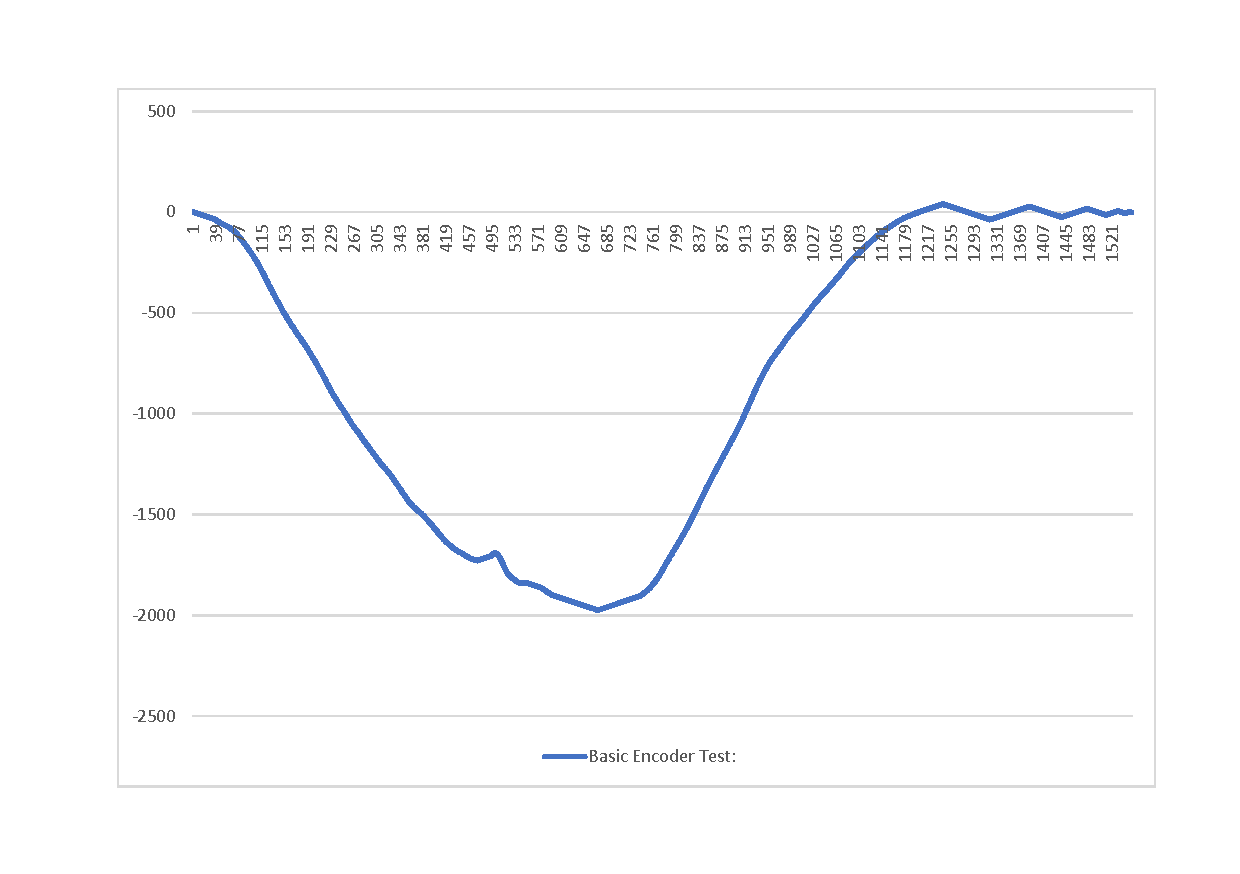
\includegraphics[width=14cm, height=10cm]{pruebasensor}
	\caption{Diagrama de adquisi'on de datos del sensor HEDM-5500}
	\label{fig:adqsens}
\end{figure}
\end{center}
\subsection{An'alisis de los datos obtenidos de los sensores}
Se puede observar una correlaci'on entre los datos obtenidos en la interfaz serial de Arduino IDE (Fig. \ref{fig:dard}) con los puntos de resoluci'on del sensor mostrados en HMI Fig. \ref{fig:dHMI}; cabe resaltar que estos datos fueron enviados a trav'es de CAN hacia el nodo central y luego a la HMI.
\begin{figure}[ht]
	\centering
		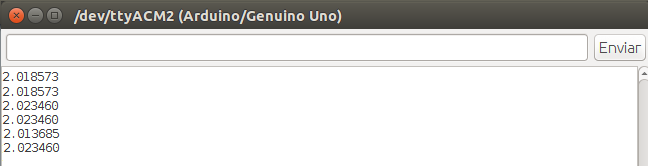
\includegraphics[scale=0.9]{datoshmi}
	\caption{Datos obtenidos por Arduino IDE}
	\label{fig:dard}
\end{figure}
\begin{figure}[ht]
	\centering
		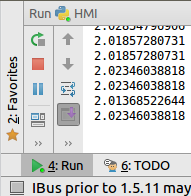
\includegraphics[scale=1]{datoshmi2}
	\caption{Datos obtenidos por HMI}
	\label{fig:dHMI}
\end{figure}

\section{Prueba del sistema simulado de control}

\subsection{Prueba del controlador en estado estable para el sistema desarrollado en Matlab}
\setlength{\parskip}{0.4cm}
En el cap'itulo anterior se mostr'o la utilidad de Matlab a la hora de obtener ganancias de un sistema en espacio de estados, tambi'en se puede a'nadir el siguiente c'odigo para obtener la simulaci'on en condiciones iniciales dadas y el tracking a una se'nal de entrada:

 {\tiny
\lstset{language=Matlab, breaklines=true, basicstyle=\footnotesize}
\begin{lstlisting}[frame=single]
%% 2. SIMULATION IN FRONT OF GIVEN CONDITIONS
x = [1; 1]; %given initial conditions
history = []; %buffer initialization
history = [history sys_d.c*x];

for i = 0 : tick : tTop
    u = -K*x; %applies control
    x = sys_d.a*x+sys_d.b*u;
    y = sys_d.c*x;
    history = [history y]; %updates buffer
end

time = 0:tick:tTop+tick;
figure
plot(time, history(1,:));
xlabel('Time [s]');
ylabel('x[1]');
legend('State');
axis([0 tTop -1 1])

%% 3. SIMULATION TRACKING A REFERENCE SIGNAL
tTop = 5;
x = [0; 0]; %given initial conditions

history = []; %buffer initialization
history = [history x];

ref = 0;
real_ref = ref - 0.5;
refHist = [];
refHist = [refHist, ref];

u = 0;
controlHist = [];
controlHist = [controlHist, u];

for i = 0 : tick : tTop
    if mod(i,1) == 0 && i ~= 0
        ref = ~ref;
        real_ref = ref - 0.5; %to simulate the behavior in the flexboards
    end
    u = K(1)*(real_ref-x(1)) - K(2)*x(2);
    x = sys_d.a*x+sys_d.b*u;
    history = [history x]; %updates buffer
    refHist = [refHist real_ref];
    controlHist = [controlHist u];
end

time = 0:tick:tTop+tick;

figure
hold on
plot(time, history(1,:));
plot(time, refHist(1,:),'color', 'red')
plot(time, controlHist(1,:),'color', 'green')
xlabel('Time [s]');
ylabel('Voltage');
legend('State','Reference','Control');
axis([0 tTop -2 2])
\end{lstlisting}
}
\subsection{Resultados adquiridos de Matlab}
A continuaci'on se muestran los datos obtenidos de Matlab
 {\tiny
\lstset{language=Matlab, breaklines=true, basicstyle=\footnotesize}
\begin{lstlisting}[frame=single]
Crank system is controllable!
Convergence was reached at
iter =  2194
Crank control gains:
K_ = [ 72.49, 25.91, 14.25, -2.096] 
KI_ = 0.9615
eigenvalues =    0.9669 + 0.0000i
   0.9817 + 0.0277i
   0.9817 - 0.0277i
   0.9920 + 0.0303i
   0.9920 - 0.0303i
\end{lstlisting}
}

\subsection{Gr'afico obtenido de la simulaci'on}
Dando como resultado que el sistema sea completamente controlable como muestra la Fig. \ref{fig:simu}:

\begin{center}
\begin{figure}[ht]
	\centering
		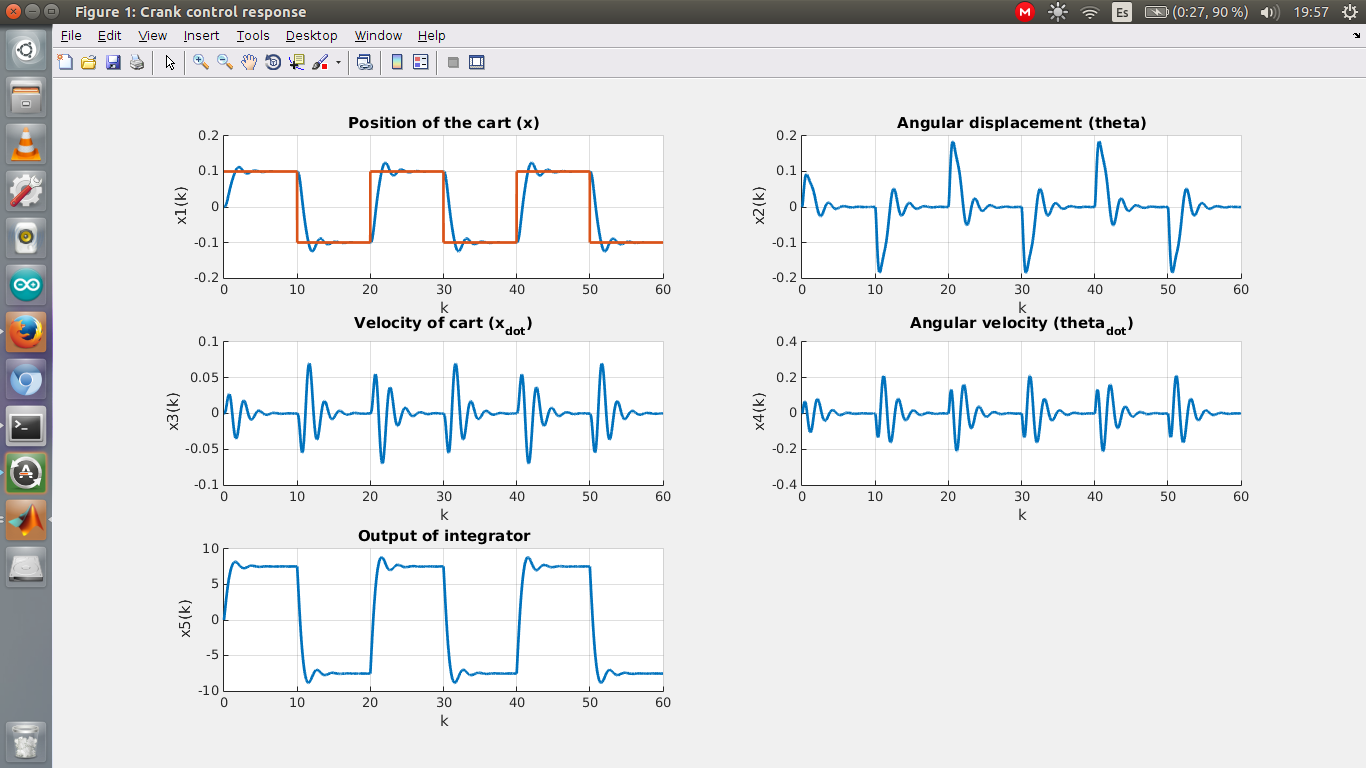
\includegraphics[width=15cm, height=10cm]{simu}
	\caption{Simulaci'on obtenida con Matlab}
	\label{fig:simu}
\end{figure}
\end{center}
\subsection{An'alisis de los resultados}
Los resultados obtenidos por Matlab muestran que el sistema es controlable, con una itinerancia de software de 2149; donde se encontraron los polos del sistema as'i como sus ganancias, las cu'ales fueron puestas en un sistema de realimentaci'on cerrado y simulado por Matlab Fig. \ref{fig:simu}.


\section{Prueba del sistema real con las ganancias obtenidas}
Prueba del sistema real con las ganancias obtenidas en el cap'itulo anterior en donde fueron modificadas para reducir el tiempo de estabilizaci'on en estado estable, dando la siguiente tabla \ref{tabla:pruebag}:

\begin{table}[htbp]
\begin{center}
\begin{tabular}{c c c c c c c}
\hline
Prueba &G1CarPos & G2CarVel& G3RosPos & G4RosVel & G5error& Tiempo Estabilizacion(seg)\\
\hline 
1 &59.86&17.9&10.17&-3.713&0.98& Inestable\\
2 &59.86&17.9&-10.17&-3.713&0.15& 20 \\
3 &59.86&17.9&-40.17&-3.713&0.15& 14 \\
4 &59.86&17.9&-40.17&-10.713&0.15& 13\\
5 &59.86&17.9&-40.17&-1.713&0.15& 15\\
6 &59.86&17.9&-40.17&-5.713&0.15& 15\\
7 &59.86&17.9&-40.17&-7.713&0.15& 14\\
8 &59.86&17.9&-40.17&-20.713&0.15& 11\\
9 &59.86&17.9&-40.17&-10.713&0.1& 14\\
10 &59.86&17.9&-40.17&-3.713&0.08& 12\\
11 &59.86&17.9&-3.17&-3.713&0.1& 20\\
12 &59.86&17.9&-40.17&-3.713&0.25& Inestable\\
\hline 
\end{tabular}
\caption{Tabla comparativa de ganancias}
\label{tabla:pruebag}
\end{center}
\end{table}

\subsection{An'alisis de los ganancias modificadas en el sistema real}
 Los datos de la tabla \ref{tabla:pruebag} muestra que las ganancias m'as cr'iticas son G3RosPos y G5error; tomando la primera valores menores a 0 el sistema se vuelve inestable y para la segunda con valores mayores a 1.5 sucede lo mismo. El mejor tiempo de estabilizaci'on se obtuvo con  G3RosPos=-40.17,G2CarVel=-20.713 y G5error =0.15 con un tiempo de estabilizaci'on de 11 seg. 


\section{An'alisis costos}
A continuaci'on se detallan los costos del trabajo realizado en la tabla \ref{tabla:costos}:

\begin{table}[htbp]
\begin{center}
\begin{tabular}{c c c c c c c c}
\hline
Egresos &Mes1&Mes2&Mes3&Mes4&Mes5&Mes6&Total\\
 &USD&USD&USD&USD&USD&USD&USD\\
\hline 
Materia prima & 200 & & & &200 && 400 \\
Mano de obra directa &  & & & & 20&& 20 \\
Mano de obra indirecta &  & & & & &&0\\
Materiales de oficina & 10 &10 &10 &5 &20 &5&60\\
\hline 
 &&&&&&Costo&480\\
&&&&&&Precio&520\\
\hline 
\end{tabular}
\caption{Tabla de costos}
\label{tabla:costos}
\end{center}
\end{table}
%\include{3controlador}
%%%%%%%%%%%%%%%%%%%%%%%%%%%%%%%%%
%\include{4hmi}
%%%%%%%%%%%%%%%%%%%%%%%%%%%%%%%%%%%
%\include{capitulo1}
%\include{capitulo2}
%\include{capitulo3}
\chapter{Conclusiones y Recomendaciones}
\section{Conclusiones}
\begin{enumerate}
	\item Los documentos recopilados referentes al control por red mostraban 'unicamente el envio y recepci'on de varios tipos de datos a trav'es de una red sin que estos documentos est'en relacionados al dise'no de controladores; por otra parte, cuando se encontraba documentaci'on relacionada al desarrollo de controladores para p'endulos, era dentro de un mismo microprocesador con el que se adquiria, procesaba, calculaba y se tomaba una acci'on de control. Por tanto en base a que no se encontr'o informaci'on completa para desarrollar este trabajo se tomaron en cuenta 4 fundamentos ampliamente desarrollados en otras tesis y son: adquisici'on y procesamiento de datos, redes CAN, HMI's y diseño de controladores.
	\item Los requerimientos necesarios para el sistema fueron tomados de documentos en los que se realizaba el control en sistemas de p'endulos invertidos pero la informaci'on relacionada a la implementaci'on de controladores en una red de campo de datos era pr'acticamente nula, por lo que la misma fu'e especialmente dise'nada y desarrollada para la planta.
	
	\item Como se muestra en  Fig. \ref{fig:simu} el sistema con las constantes establecidas en el trabajo previo es totalmente controlable. La misma simulaci'on nos da como resultado ganancias aproximadas para el sistema de control, las que sirvieron de base para el controlador real implementado con el que se hicieron las pruebas correspondientes.
	\item La adquisici'on, monitoreo y control de datos fue realizada como se muestra en la Fig. \ref{fig:HMI} y es consecuente con lo planteado en el dise'no de la misma para el control desde la PC para toda la red. La interfaz se pus'o a prueba mientras se modificaban las ganancias para el controlador; as'i como para la adquisici'on y monitoreo de los datos provenientes de la red. 
	\item Despu'es de haber implementado la red, HMI y el controlador para el sistema, las pruebas fueron realizadas y se pudieron obtener varios valores donde las ganancias estabilizan la planta.
\end{enumerate}

\section{Recomendaciones}
\subsection{Recomendaciones del sistema electr'onico}
\begin{enumerate}
	\item El correcto funcionamiento de la planta con Arduino Uno muestra la efectividad en cuanto a trabajo de procesamiento que tienen estos shields y control que proveen para con los sensores; sin embargo se recomienda el uso y desarrollo en Arduino Due o Mega que cuentan con m'as pines para interrupciones externas que podr'ian ser usados para conectar los canales A y B de cada uno de los encoders para mejorar el rendimiento del sistema.
	\item Habr'ia que cambiar los shields de comunicaci'on CAN si se usan algun otro tipo de shield de control, ya que los que est'an montados en la red son exclusivos para los Arduinos Uno o en su defecto manufacturar un shield propio.
	
\end{enumerate}
\subsection{Recomendaciones del sistema de control}
\begin{enumerate}
	\item El sistema podr'ia responder de manera m'as o menos estable, dependiendo de las ganancias que sean calculadas a posteriori para el mismo controlador o para controladores que sean implementados con diferentes t'ecnicas de dise'no de controladores.
	\item Para posteriores trabajos se deber'ia tomar en cuenta los tiempos de propagaci'on dentro del sistema de comunicaci'on CAN, aquellos que afectan al sistema de control de la planta.
	\item Realizar las modificaciones del sistema de control dentro de los nodos para conseguir la estabilizaci'on del sistema en alto.
\end{enumerate}
\subsection{Recomendaciones para la HMI}
\begin{enumerate}
	\item Se podr'ia utilizar la HMI para trabajos no tan rigurosos, a'un que la proyecci'on es utilizarlo como punto de convergencia para intercambiar controladores sin tener que desmontar totalmente la red.
	\item Se podr'ian mostrar m'as datos en la pantalla de la HMI que por el momento no son necesarias.
	\item No utilizar mas de dos conectores USB al momento de correr el programa en Python, ya que puede causar fallas en la HMI.
	
\end{enumerate}
\subsection{Otras recomendaciones}
\begin{enumerate}
	\item Si se trata de conseguir la estabilizaci'on en alto se aconseja reaalizar el desarrollo matem'atico de la planta as'i como de su simulaci'on previo a la implementaci'on de la misma. 
	\item Como parte integral del desarrollo de este trabajo se utiliz'o la herramienta Latex para el documento escrito; por lo que se recomienda utilizarlo en posteriores trabajos.
\end{enumerate}
 
 

%\include{apendiceB}
%\include{apendiceC}

%% Incluir la bibliograf'ia. Mirar el archivo "biblio.bib" para m'as detales
%% y un ejemplo.
%\clearpage
%\printglossary[title=Special Terms, toctitle=List of terms]


\bibliography{biblio}


\appendix
 \renewcommand\appendixname{Anexos}
%  \renewcommand\appendixpagename{Anexos}

 
\chapter{\normalsize Can Bus Shield Sparfun Schematic}

\begin{center}
  \includegraphics[scale=0.6]{canbus_shield-v12}  
	
\end{center}
\chapter{\normalsize Programa base para la HMI en Python}
\vspace{0cm}
Autores: Carlos Xavier Rosero, Manel Velasco Garc'ia. Nombre y extensi'on de archivo: \textbf{\textit{testDimitris.py}}.
{\tiny
\begin{lstlisting}[language=python]
#!/usr/bin/env python
# -*- coding: utf-8 -*-
"""
@authors: carlos xavier rosero
          manel velasco garc�a

best performance tested with python 2.7.3, GCC 2.6.3, pyserial 2.5
"""
from __future__ import division

import serial, struct
from collections import deque
import time

import matplotlib.pyplot as plt
import matplotlib.animation as animation

class command:
    startCx = 0xf0
    stopCx = 0xf1


#use this part only with old versions of python and libraries
#tested specifically with python 2.6.5, GCC 4.4.3, serial 1.3.5
class adapt(serial.Serial):
    def write(self, data):
        super(self.__class__, self).write(str(data))

class serialCx:

    def __init__(self, usbPort, frameLen, maxLen, EOL, bauds):

        self.ay1 = deque([0.0]*maxLen)
        self.ay2 = deque([0.0]*maxLen)

        self.maxLen = maxLen

        self.eol = EOL #end of line
        self.lenEol = len(self.eol) #length of the end of line

        self.frameLen = frameLen - self.lenEol

        self.float0 = float(0)
        self.float1 = float(0)

        # open serial port
        self.ser = adapt(port=usbPort, baudrate=bauds, timeout=1, parity=serial.PARITY_NONE,
                stopbits=serial.STOPBITS_ONE)

        self.ser.open
        self.ser.isOpen

        time.sleep(2) #waits until arduino gets up

        inputS = [] #initializes buffer
        while self.ser.inWaiting() > 0: #neglects the trash code received
            inputS.append(self.ser.read(1)) #appends a new value into the buffer

        
        self.float0ToTx = float(9.5)  #initial values of the floating numbers to be sent
        self.float1ToTx = float(-9.5)

        value0 = struct.pack('%sf' % 1, self.float0ToTx) #splits the float value into 4 strings
        value1 = struct.pack('%sf' % 1, self.float1ToTx) #splits the float value into 4 strings

        #this buffer sends the command to start tx from arduino and both floating registers
        buffer = bytearray([command.startCx, ord(value0[0]), ord(value0[1]), ord(value0[2]), ord(value0[3]),
                                             ord(value1[0]), ord(value1[1]), ord(value1[2]), ord(value1[3])])

        self.ser.write(buffer) #sends the command to start the reception


  # add to buffer
    def addToBuf(self, buf, val):
        if len(buf) < self.maxLen:
            buf.append(val)
        else:
            buf.pop()
            buf.appendleft(val)

    # update plot
    def update(self, frameNum, a1, a2):
        line = bytearray()
        try:
            while True:
                c = self.ser.read(1)
                if c:
                    line.append(c)
                    if line[-self.lenEol:] == self.eol: #verifies if EOF has been received
                        line = line[0:-self.lenEol] #removes EOF
                        break
                else:
                    break

            if len(line) == self.frameLen:

                self.float0 = struct.unpack('f', line[0:4])
                self.float0 = self.float0[0] #takes out the only one element from the tuple

                self.float1 = struct.unpack('f', line[4:8])
                self.float1 = self.float1[0] #takes out the only one element from the tuple

                print self.float0,
                print self.float1

                # add data to buffer
                self.addToBuf(self.ay1, self.float0)
                self.addToBuf(self.ay2, self.float1)

                a1.set_data(range(self.maxLen), self.ay1)
                a2.set_data(range(self.maxLen), self.ay2)

            else:
                print 'Incorrect frame length:',
                print len(line)
                self.ser.flushInput() #gets empty the serial port buffer

        except KeyboardInterrupt:
            print('Exiting...')

    # clean up
    def close(self):
        # close serial

        buffer = bytearray([command.stopCx, 0x01, 0x01, 0x01, 0x01, 0x01, 0x01,
                            0x01, 0x01]) #the (0x01) is used only to fill the buffer
                                         #in order to accomplish the standard length

        self.ser.write(buffer) #sends the command to start the reception

        self.ser.flushInput()
        self.ser.close()

def plotting(givenData):

    fig = plt.figure()

    ax1 = plt.subplot(211)
    ax1.grid(True)
    a1, = ax1.plot([0], [0], color=(0, 1, 0))
    plt.xlim(0, 200)
    plt.ylim(-10, 10)
    plt.ylabel('Float 0')

    ax2 = plt.subplot(212)
    ax2.grid(True)
    a2, = ax2.plot([0], [0], color=(0, 1, 0))
    plt.xlim(0, 200)
    plt.ylim(-10, 10)
    plt.ylabel('Float 1')

    anim = animation.FuncAnimation(fig, givenData.update, fargs=(a1, a2), interval=50)

    plt.show() # show plot

#######################################
######here starts the main program#####
#######################################
if __name__ == "__main__":

    testCarlos = serialCx('/dev/ttyACM9', 12, 200, 'cXrC', 115200)
    plotting(testCarlos)
    serialCx.close(testCarlos)
\end{lstlisting}

}



\chapter{\normalsize Programa base para el desarollo del Nodo 0 en Arduino,}
\vspace{0cm}
Autores: Carlos Xavier Rosero, Manel Velasco Garc'ia, incluidas librer'ias propias de arduino. Nombre y extensi'on de archivo \textit{\textbf{testDimitris.ino}}.

 {\tiny


\begin{lstlisting}[language=python]
boolean txOn = false;  // whether the frame is complete
unsigned char counterRx = 0;
unsigned char bufferRx[20] = {0,0,0,0,0,0,0,0,0,0,0,0,0,0,0,0,0,0,0,0};
float float0 = 0; //numbers to be sent
float float1 = 0;
unsigned char *pointer_float0 = (unsigned char *)&float0;
unsigned char *pointer_float1 = (unsigned char *)&float1;
float float2 = 0; //numbers to be received
float float3 = 0;
float *pointer_float2 = (float *)&bufferRx[1];
float *pointer_float3 = (float *)&bufferRx[5];
void setup()
{
  Serial.begin(115200);   // initialize serial:
  pinMode(13,OUTPUT);
  digitalWrite(13,LOW);
}
void loop()
{
  unsigned char i; 
  unsigned char data0[4] = {0xcd, 0xcc, 0x0c, 0x40};
  unsigned char data1[4] = {0xcd, 0xcc, 0x4c, 0x40};
  unsigned char eof[4] = {'c','X','r','C'};
  if (txOn)
  {
    for (i=0; i<4; i++)
			Serial.write(pointer_float0[i]);
    for (i=0; i<4; i++)
      Serial.write(pointer_float1[i]);
    for (i=0; i<4; i++)
      Serial.write(eof[i]);
  }
  delay(100);
  float0 = float2;
  float1 = float3;
}
void serialEvent()
{
  while (Serial.available())
  {
    bufferRx[counterRx] = (unsigned char)Serial.read(); //get the new byte
    if (counterRx >= 8)
    {
      counterRx = 0;
       digitalWrite(13, !digitalRead(13)); //toggles led each time the buffer is 9 bytes long
      switch (bufferRx[0]) //analyze command on first byte
      {
        case 0xf0:
          txOn = true;
          //here make a union of bytes to build the float registers
          float2 = (*pointer_float2);
          float3 = (*pointer_float3);           
        break;
        case 0xf1:
          txOn = false;
        break;
      } 
    }
    else
      counterRx++;
  }
}
\end{lstlisting}

}





%% Cap'itulos incluidos despues del comando \appendix aparecen como ap'endices
%% de la tesis.
%\include{apendiceA}
\end{document}
